\documentclass{report}
\usepackage[utf8]{inputenc}
\usepackage{url}            % simple URL typesetting
\usepackage{booktabs}       % professional-quality tables
\usepackage{wrapfig}
\usepackage{nicefrac}       % compact symbols for 1/2, etc.
\usepackage{amsfonts}       % blackboard math symbols
\usepackage{graphicx}
\usepackage{hyperref}       % hyperlinks
\usepackage{algorithmic}
\usepackage{natbib}
\usepackage{subcaption}
\usepackage{amsthm}
\usepackage{amsmath}
\usepackage{amssymb}
\usepackage{mathtools}
\usepackage{bm}
\usepackage{kky}
\usepackage[a4paper, total={6in, 8in}]{geometry}
\newtheorem{prop}{Prop.}
\providecommand*\theoremautorefname{Theorem}

\usepackage[ruled,vlined]{algorithm2e}
\usepackage[symbols,nogroupskip,sort=none]{glossaries-extra}

\newcommand{\notation}[3]{\glsxtrnewsymbol[description={#1}]{#2}{\ensuremath{#3}}}
\newcommand{\aka}{{\em a.k.a.~}}
\newcommand{\ybu}{\underline{\yb}}
\newcommand{\xbu}{\underline{\xb}}
\newcommand{\sbbu}{\underline{\sbb}}
\newcommand{\eps}{\varepsilon}
\DeclareMathOperator{\GL}{GL}


\title{
  {Thesis Title}\\
  {\large Institution Name}\\
  {\includegraphics{university.jpg}}
}
\author{Author Name}
\date{Day Month Year}


\begin{document}

\notation{Number of views}{m}{m \in \NN}
\notation{Number of components}{p}{p \in \NN}
\notation{Number of samples}{n}{n \in \NN}
\notation{Data of view $i$}{xbi}{\xb_i \in \RR^{p}}
\notation{$j$-th entry of $\xb_i$}{xbij}{x_{ij} \in \RR}
\notation{Shared components}{sbb}{\sbb \in \RR^{p}}
\notation{$j$-th entry of $\sbb$}{sj}{s_j \in \RR}
\notation{Mixing matrix of view $i$}{Ai}{A_i \in \RR^{p \times p}}
\notation{Unmixing matrix of view $i$}{Wi}{W_i \in \RR^{p \times p}}
\notation{Absolute value of the determinant of $W_i$}{detWi}{|W_i|}
\notation{Unmixed data of view $i$: $\yb_i = W_i \xb_i$}{ybi}{\yb_i}
\notation{Noise of view $i$}{ni}{\nb_i \in \RR^{p}}
\notation{Covariance of $\nb_i$}{Sigmai}{\Sigma_i \in \RR^{p \times p}}
\notation{$j, j$ entry of a diagonal matrix $\Sigma_i$}{Sigmaij}{\Sigma_{ij} \in \RR}
\notation{Global noise level $\sigma^2 = \frac1{mp} \sum_i \tr(\Sigma_i)$}{sigma}{\sigma \in \RR}
\notation{For a scalar valued function $f$ and a vector $\sbb$, $f(\sbb) = \sum_{j=1}^kf(s_j)$}{fs}{f(\sbb)}
\notation{For a scalar valued function $f$, $f'(\sbb)$ is the gradient of $\xb
  \rightarrow f(\xb)$ at value $\sbb$}{gf}{f'(\sbb)}
\notation{Identify matrix}{I}{I_p \in \RR^{p \times p}}
\notation{Expectation}{E}{\EE}
\notation{Variance}{V}{\VV}
\notation{Density of random vector $\sbb$}{psbb}{p_{\sbb}(\cdot)}
\notation{Trace}{tr}{\tr}
\notation{Set of $p \times p$ invertible matrices}{glp}{\GL_p}
\notation{Number of elements in the set $\mathcal{S}$}{card}{|\mathcal{S}|}
\notation{Gradient}{grad}{\mathcal{G}}
\notation{Hessian}{hess}{\mathcal{H}}

% \chapter*{Abstract}
% Abstract goes here

% \chapter*{Dedication}
% To mum and dad

% \chapter*{Declaration}
% I declare that..

% \chapter*{Acknowledgements}
% I want to thank...

\tableofcontents
\printunsrtglossary[type=symbols,style=long, title=Notations]


% \paragraph{Notations} We write vectors in bold letter $\vb$ and scalars in lower case $a$. Upper case letters $M$ are used to denote
% matrices. We denote $|W|$ the absolute value of the determinant of $W$. $\xb \sim \Ncal(\mub, \Sigma)$ means that $\xb \in \mathbb{R}^k$ follows
% a multivariate normal distribution of mean $\mub \in \mathbb{R}^k$ and
% covariance $\Sigma \in \mathbb{R}^{k \times k}$. The $j, j$ entry of a diagonal matrix $\Sigma_i$ is denoted $\Sigma_{ij}$, the $j$ entry of $\yb_i$ is denoted $y_{ij}$. Lastly, $\delta$ is the Kronecker delta.
% \textbf{Notation} The absolute value of the determinant of a matrix $W$ is $|W|$.
% % 
% The $\ell_2$ norm of a vector $\sbb$ is $\|\sbb\|$.
% % 
% For a scalar valued function $f$ and a vector $\sbb \in \bbR^p$, we write $f(\sbb) = \sum_{j=1}^kf(s_j)$ and denote $f'$ the gradient of $f$.

\chapter{Introduction}
\section{Probabilistic models}
\subsection{Identifiability}
\subsection{Maximum likelihood}
\section{Optimization}
\subsection{Gradient descent, Newton, Quasi-Newton}
\subsection{EM and generalized EM}
\section{Independent component analysis}
\subsection{Non Gaussian ICA}
\subsubsection{Identifiability}
\subsubsection{Robustness to density missmatch}
\subsubsection{Stability (extended infomax)}
\subsection{non-stationary ICA}
\subsubsection{Identifiability}
\subsubsection{Joint diagonalization objective}
\subsection{Dimension reduction}
So far, we have assumed that the dimensionality of the data $v$ and the number
of components $p$ is the same. 
In practice, however, we might want to estimate fewer components than there are observations per view; the original dimensionality of the data %(number of voxels, sensors) 
might in practice not be computationally tractable.

% The problem of how to perform subject-wise dimensionality reduction in group studies 
% % of data for each of the individuals while still considering them jointly and preserving the signal shared across them
% is an interesting one \emph{per se}, and out of the main scope of this work. For our purposes, it can be considered as a preprocessing step for which well-known various solutions can be applied. % step prior to the application of our method,. 
% We discuss this further in section~\ref{sec:rel_work} and in appendix~\ref{sec:app_rel_work}.

A classical approach to perform dimension reduction is principal component
analysis (PCA) which we now present.
Our data is represented as a random vector $\xb \in \bbR^v$ that is assumed
centered ($\EE[\xb] = 0$). Take $C = \Cov(\xb) \in \mathbb{R}^{v \times v}$ the
covariance of $\xb$ and compute an eigenvalue decomposition $VD^2V {\top} = C$
such that the coefficients of the diagonal matrix $D^2 \in \mathbb{R}^{v
  \times v}$ are ordered in decreasing order and $V$ is an orthogonal matrix.
Then $V = [\vb_1 \dots \vb_m]$ gives the projection vectors such that the $p$ first
principal components are then given by $[\vb_1 \dots \vb_p]^{\top} \xb$. Note
that our formulation of PCA does not include whitening of the signals.



% For a zero-mean data matrix $X$ of size $p\times n$ with $p \leq n$, we denote $X= UD V^{\top}$ the singular value decomposition of $X$ where $U \in \bbR^{p\times p}$, $V \in \bbR^{n \times p}$ are orthogonal and $D$ the diagonal matrix of singular values ordered in decreasing order.
% The PCA of $X$ with $k$ components is $Y\in\bbR^{k\times n}$ containing the
% first $k$ rows of $DV^{\top}$, and it does not hold in general that
% $YY^{\top}=I_k$: in this thesis, what we cann PCA does not include whitening of the signals.
\section{Analysis of MultiView data}
Many methods for data-driven multivariate analysis of neuroimaging group studies have been proposed. We summarize the characteristics of some of the most commonly used ones. A more thorough description of these methods can be found in appendix~\ref{sec:app_rel_work}.
\subsection{Group independent component analysis}
\subsubsection{Likelihood based method}
One can consider the more general model $\xb_i = A_i\sbb^i + \nb_i$, where the noise covariance can be learned from the data~\cite{guo2008unified}.
% 
Having the simpler model~\eqref{eq:mvica:model} leads to a closed-form likelihood, that can then be optimized by more efficient means than the EM algorithm.
In model~\eqref{eq:mvica:model}, the noise can be interpreted as individual variability rather than sensor noise. %It offers a way to capture more structured noise as is often the case in brain signals.
% It offers a way to capture more structured noise, which is often present in neuroimaging recordings~\cite{engemann2015automated}.
In appendix~\ref{app:complex_cov}, we generate data following model $\xb_i = A_i\sbb^i + \nb_i$ and report the reconstruction error. The difference in performance between algorithms is small. 
\subsubsection{CanICA}
\cite{varoquaux2009canica}

\subsubsection{ConcatICA}
When datasets are high-dimensional, a three steps procedure is often used: first dimensionality reduction is performed on data of each subject  separately; then the reduced data are merged into a common representation; finally, an ICA algorithm is applied for shared components extraction. The merging of the reduced data is often done by PCA \cite{calhoun2001method} or multi set CCA \cite{varoquaux2009canica}.
%Note that even with large datasets, it can still be computationally feasible to do group level reduction in one step (see \cite{chen2015reduced} or \cite{smith2014group}).
This is a popular method for fMRI~\cite{calhoun2009review} and EEG~\cite{eichele2011eegift} group studies.
These methods directly recover only group level, shared components; when individual components are needed, additional steps are required (back-projection \cite{calhoun2001method} or dual-regression \cite{beckmann2009group}).
%
In contrast, MultiView ICA finds individual and shared independent components in a single step.
%
%
Finally, in contrast to the methods described above, our method maximizes a likelihood, which brings statistical guarantees like consistency or asymptotic efficiency.
\subsection{Independent vector analysis}
\subsubsection{IVA-L}
\subsubsection{IVA-G}
\subsection{Shared response modeling}
\subsubsection{Hyperalignment}
\subsubsection{Deterministic SRM}
\subsubsection{Probabilistic SRM}
\subsection{Multiset CCA}


% \section{Related Work}
% \label{sec:rel_work}
% %

% %
% %

% %
% %
% %

% \textbf{Structured mixing matrices} One strength of our model is that we only assume that the mixing matrices are invertible and still enjoy identifiability whereas some other approaches impose additional constraints. For instance tensorial methods~\cite{beckmann2005tensorial} assume that the mixing matrices are the same up to diagonal scaling.
% %
% Other methods impose a common mixing matrix~\cite{cong2013validating, grin2010independent, calhoun2001fmri, Monti18UAI}. Like PCA, the Shared Response Model~\cite{chen2015reduced} (SRM) assumes orthogonality of the mixing matrices. While the model defines a simple likelihood and provides an efficient way to reduce dimension, the SRM model is not identifiable as shown in appendix~\ref{sec:app_identifiability}, and the orthogonal constraint may not be plausible.
% %

% \textbf{Matching components a posteriori} A different path to multi-subject ICA is to extract independent components with individual ICA in each subject and align them. We propose a simple baseline approach to do so called \emph{PermICA}.
% Inspired by the heuristic of the hyperalignment method~\cite{haxby2011common} we choose a reference subject and first match the components of all other subjects to the components of the reference subject. The process is then repeated multiple times, using the average of previously aligned components as a reference. Finally, group components are given by the average of all aligned components. We use the Hungarian algorithm to align pairs of mixing matrices~\cite{tichavsky2004optimal}.
% %
% Alternative approaches involving clustering have also been developed~\cite{esposito2005independent,bigdely2013measure}.

% \textbf{Deep Learning} Deep Learning methods, such as convolutional auto-encoders (CAE), can also be used to find the subject specific unmixing~\cite{chen2016convolutional}. While these nonlinear extensions of the aforementioned methods are interesting, these models are hard to train and interpret. In the experiments on fMRI data in appendix~\ref{appendix_reproduce}, we obtain better accuracy with MultiView ICA than that of CAE reported in~\cite{chen2016convolutional}.

% \textbf{Correlated component analysis} Other methods can be used to recover the shared neural responses such as the correlated component approach of Dmochowski~\cite{dmochowski2012correlated}. We benchmark our method against its probabilistic version~\cite{kamronn2015multiview} called BCorrCA in Figure~\ref{fig:meg}. Our method yields much better results. 

% \textbf{Autocorrelation} Another way to perform ICA is to leverage spectral diversity of the components rather than non-Gaussianity.
% %
% These methods are popular alternative to non-Gaussian ICA in the single-subject setting~\cite{tong1991indeterminacy, belouchrani1997blind, pham1997blind} and they output significantly different components than non-Gaussian ICA~\cite{delorme2012independent}.
% %
% Extensions to multiview problems have been proposed~\cite{lukic2002ica, congedo2010group}.
% \vspace{-5pt}
\chapter{FastSRM}

\chapter{MultiViewICA}
\section{Introduction}
% The past decade has seen the emergence of two trends in neuroimaging: the collection of massive neuroimaging datasets, containing data from hundreds of participants~\cite{taylor2017cambridge,van2013wu,sudlow2015uk}, and the use of naturalistic stimuli to move closer to a real life experience with dynamic and multimodal stimuli~\cite{Sonkusare-etal:2019}.
% %
% % The analysis of these datasets is typically unsupervised when task and/or stimulation are difficult to quantify, such as in movie watching, yet this type of analysis offers insights on human brain function and useful individual markers.
% %
% Large scale datasets provide an unprecedented opportunity to assess the generality and validity of neuroscientific findings across subjects, with the potential of offering novel insights on human brain function and useful medical biomarkers.
% %
% % However, the analysis of such data is highly nontrivial --- particularly so when task and/or stimulation are difficult to quantify, such as in presence of natural stimuli.
% %
% However, when using ecological conditions, such as movie watching or simulated driving, 
% stimulations are difficult to quantify. Consequently the statistical analysis of the data using
% supervised regression-based approaches is difficult.
% %
% This has motivated the use of unsupervised learning methods that leverage the availability of
% data from multiple subjects performing the same experiment; analysis on such large groups boosts statistical
% power.

% Independent component analysis~\cite{hyvarinen2000independent} (ICA) is a widely used unsupervised method for neuroimaging studies. It is routinely applied on individual subject electroencephalography (EEG)~\cite{makeig1996independent}, magnetoencephalography (MEG)~\cite{vigario1998independent} or functional MRI (fMRI)~\cite{mckeown1998independent} data. 
% %
% ICA models a set of signals as the product of a \emph{mixing matrix} and a \emph{components} matrix containing independent components.
% %
% The identifiability theory of ICA states that having non-Gaussian independent components is a strong enough condition to recover the model parameters~\cite{comon1994independent}.
% %
% ICA therefore does not make assumptions about what triggers brain activations in the stimuli, unlike confirmatory approaches like the general linear model \cite{friston1994statistical, poline2012general}.
% %
% This explains why, in fMRI processing, it is a model of choice when analysing
% resting state data \cite{beckmann2005investigations} or when subjects are
% exposed to natural~\cite{malinen2007towards}~\cite{bartels2005brain} or complex stimuli such as simulated driving \cite{calhoun2002different}.
% In M/EEG processing, it is widely used to isolate acquisitions artifacts from neural signal~\cite{jung1998extended}, and to identify brain components of interest~\cite{vigario2000independent, delorme2012independent}.
% % Besides, these models are typically univariate, thus not exploiting structure in the data, and lose statistical power in the presence of structured noise non orthogonal to the data.

% %ICA is a tool of interest to conduct group studies.
% %\bt{ICA is not primarily a group studies tool}
% %
% %\bt{From now on, you are implicitly assuming that components are in the time domain, and mixing is spatial. Maybe worth mentioning.}\pa{On the contrary I think we should not restrict ourselves to such case. To me, we propose a novel way to perform group ica on any type of data.}
% %
% However, unlike with univariate methods, statistical inference about multiple subjects using ICA is not straightforward: so-called group-ICA is the topic of various studies~\cite{hyvarinen2013independent}.
% %
% Several works assume that the subjects share a common mixing matrix, but with different components~\cite{pfister2019robustifying}~\cite{svensen2002ica}.
% %
% Instead, we focus on a model where the subjects share a common components matrix, but have different mixing matrices.
% %
% When the subjects are exposed to the same stimuli, the common components matrix corresponds to the group \emph{shared responses}.
% %\bt{Oops: for spatial ICA, this has been done for some time with models such as CanICA}
% %
% Most methods proposed in this framework proceed in two steps~\cite{calhoun2009review, huster2015group}.
% %
% First, the data of individual subjects are aggregated into a single dataset, often resorting to dimension reduction techniques like Principal Component Analysis (PCA).
% %
% Then, off-the-shelf ICA is applied on the aggregated dataset.
% %
% This popular method has the advantage of being simple and
% straightforward to implement since it resorts to customary single-subject
% ICA method.
% %
% However, it is not grounded in a principled probabilistic model of the problem, and does not have strong statistical guarantees like asymptotic efficiency. %\bt{Clarify what guranatees we're talking about ?}.
% %
% %Some ICA based neuroimaging studies aim at drawing general conclusions on brain organization \citep{allen2014tracking, sockeel2016large} or on brain's response to a presented stimulus \citep{van2008visual} given the observation of a cohort of subjects while others focus on the difference between brains of different groups of patients based for example on age \cite{kohler2008spatiotemporal} or mental health conditions \citep{assaf2010abnormal, jafri2008method, broyd2009default}. These studies use extensions of ICA that allows its application on groups. Note that groups are not necessarily groups of subjects, they can for example be groups of trials or sessions.
% %
% %Many group ICA methods exist (see the reviews for fMRI \citep{calhoun2009review, schmitthort2004comparison, guo2008unified} and EEG \citep{huster2018tutorial, huster2015group}). Most methods start by reducing the data of each subject separately using for instance a PCA. Then the reduced data are then merged before ICA is applied on the merging. Different techniques for merging lead to different methods the most popular being the GroupICA method implemented in GIFT \cite{calhoun2001method}. In GIFT, reduced data are merged using one or sometimes two \cite{erhardt2011comparison} successive applications of PCA.
% %

% We propose a novel group ICA method called \emph{MultiView ICA}.
% %
% It models each subject's dataset as a linear combination of a common
% components matrix with additive Gaussian noise.
% %
% Importantly, we consider that the noise is on the components and not on
% the sensors.
% %
% This greatly simplifies the likelihood of the model which can even be
% written in closed-form.
% %
% % Despite its simplicity, our model can account for distinct covariances across subjects.
% Despite its simplicity, our model allows for an expressive representation of inter-subject variability through subject-specific functional topographies (mixing matrices) and variability in the individual response (with noise in the components domain).
% %
% %\bt{no justification from a modeling perspective ?} \pa{I don't have a clear view of a scenario where it is more plausible than noise on the sensors, but it would definitely be good to have such example. Maybe talk about the rosetta stone problem?}
% %
% To the best of our knowledge, this is the first time that such a tractable likelihood is proposed for multi-subject ICA.
% %
% The likelihood formulation shares similarities with the usual ICA likelihood, which allows us to develop a fast and robust alternate quasi-Newton method for its maximization.


% \textbf{Contribution}
% %
% In section~\ref{sec:mvica}, we introduce the MultiView ICA model, and show that it is identifiable. We then write its likelihood in closed form, and maximize it using an alternate quasi-Newton method.
% %
% We also provide a sensitivity analysis for MultiView ICA, and show that the choice of the noise parameter in the algorithm has little influence on the output.
% %
% In section~\ref{sec:rel_work}, we compare our approach to other group ICA methods.
% %
% Finally, in section~\ref{sec:expts}, we empirically verify through extensive experiments on fMRI and MEG data that it improves components identification with respect to competing methods, suggesting that the expressiveness and robustness of our model make it a useful tool for multivariate neural signal analysis.

%In section~\ref{sec:mvica}, we present our model and describe the optimization algorithm. We also analyze the robustness of our proposed procedure to model misspecification.
%In section~\ref{sec:rel_work}, we comment on the relationship between our work and other previously proposed models.
%In section~\ref{sec:expts}, we present an extensive experimental validation, on both synthetic and real data.
%In section~\ref{sec:conclusions}, we summarize our conclusions.



% (autism spectrum disorder \cite{assaf2010abnormal}, schizophrenia \cite{jafri2008method} see \cite{broyd2009default} for a complete review on studies linking default mode network abnormalities and mental disorders).

%It is often desirable to draw general conclusions on the response of the brain to a presented stimulus \cite{van2008visual} or on brain organization \cite{}  given the observation of individual responses in a large cohort of subjects.


%Group studies are one of the chief tools for this analysis: the aim is to draw general conclusions on the response of the brain to a presented stimulus given the observation of individual responses in a large cohort of subjects \addref. The availability of data coming from large number of individuals is critical for drawing valid conclusions about the functional organization of the human brain \addref.
%However, the aggregation of data coming from different subjects presents many challenges, ranging from the high variability in both the anatomy and the functional organization of the brain across subjects to the variability in the stimulus elicited response. 

% A first issue is the high variability in both the anatomy and the functional organization of the brain across subjects. While there are many methods to perform anatomical alignment, it is known that anatomical alignment does not correspond to alignment of functional topographies \addref. Furthermore, these procedures can imply a loss of relevant information, particularly when performed on high-resolution data. 
% Other problematic aspects have to do with the necessity of accounting for variability in the stimulus response, and also intra-subject variability as well when considering multiple presentations of the same stimulus --- %. 
% While the notion of a shared response to a given stimulus can be useful
% since the response evoked in each individual by a given stimulus might be affected by contingent factors (e.g. attention level, level of caffeine in the blood etc.), thus making the task of extracting the shared component of the response harder\addref. %Furthermore, the data relative to each of the subjects might be noisy and affected by experimental errors.

% The statistical analysis of data coming from multiple subjects should therefore ideally account for all of the above factors, using data coming from a group of individuals to extract a representation of the shared response. 

% A desirable feature of such representation would be interpretability; that is, distinct functional brain modules involved in the shared response should be distinguishable within the extracted representation.

%A popular alternative approach for tackling this problem is to employ an unsupervised learning scheme to extract the shared response. Independent component analysis \addref models the observed data as the linear mixing of a multivariate latent vector of features, whose components are assumed to be independent. This model has been widely used for feature extraction in neuroimaging studies \addref, has a clear likelihood formulation with strong identifiability guarantees, and efficient optimization procedures have been developed for it. While the basic framework is only directly applicable on individual subjects, many extensions to multi-subject data exist \addref; however, these approaches typically either lack a proper likelihood formulation or are very computationally demanding\addref
%Alternatively, models based on principal component analysis or canonical correlation analysis can be employed --- such as, for example, the shared response model~\cite{chen2017shared} (SRM); %provides a simple but effective framework to analyse fMRI data of subjects exposed to naturalistic stimuli.
%however, in order to retain computational efficiency, strong restrictions in generality are often imposed on the expressiveness of the model, which result in a lack of identifiability \luigi{should we mention it here? The fact that SRM is not identifiable is an original result of Pierre's}.
% namely imposing orthogonality of the unmixing matrices.
%
%
%\section{Shared Response Modeling (SRM)}
%\label{sec:sharedresponsemod}
%\input{sec/sharedresponsemod}
%
%
\section{Multiview ICA for Shared response modelling}
\label{sec:mvica}
\subsection{Model, likelihood and approximation}
$\xb_1, \dots ,\xb_m \in \bbR^p$ denote the $m$ observed random vectors obtained from the $m$ different views. We posit the following generative model for $i= 1\dots m$
\begin{align}
   &\xb_i = A_i(\sbb + \nb_i) \\
   & \nb_i \sim\mathcal{N}(0, \sigma^2 I) \label{eq:mvica:model} 
\end{align}
where $\sbb \in \mathbb{R}^{p}$ contains the latent variables giving the \emph{shared components}, $A_1,\dots, A_m\in\bbR^{p\times p}$ are \emph{mixing matrices}, $\nb_i \in
\mathbb{R}^{p}$ are \emph{individual noises} and the hyper-parameter $\sigma$ defines the
\emph{global noise level}.

The assumption of additive white noise on the sources models individual deviations from the shared sources $\sbb$.
It is equivalent to having noise on the sensors with covariance $\sigma^2 A^i \left(A^i\right)^{\top}$, i.e. a scaled version of the data covariance without noise.

In this chapter, we make the classical ICA assumptions: the mixing matrices are invertible $\forall i, A_i \in \GL_p$, the shared components are
statistically independent $p_{\sbb}(\sbb) = \prod_{j=1}^p p_{s_j}(s_j)$ and at most one component is Gaussian. 

Since the components are shared by the views, there are many more observed variables than components in the model: there are $p$ components, while there are $p \times m$ observations.
Therefore, MultiViewICA can be seen as an instance of \emph{undercomplete} ICA.
%

The goal of MultiViewICA is to recover the mixing matrices $A_i$ from observations of the $\xb_i$.
The following proposition extends the standard idenfitiability theory of ICA~\cite{comon1994independent} to multiview ICA, and shows that recovering the components/mixing matrices is a well-posed problem up to scale and permutation.
%
\begin{proposition}[Identifiability of MultiView ICA]
\label{prop:identifiability}
Consider $\xb_i, \enspace i=1\dots m,$ generated from~\eqref{eq:mvica:model}
with parameters $A_i$. Assume that there exists another set of parameters
$A'_i$ that also generates $\xb_i$ under the same model.
Then, there exists a permutation matrix $P\in \bbR^{k\times k}$ such that for all $i$, $A'_i = A_i P$.
\end{proposition}
Proof in Appendix~\ref{app:proof:mvica:identifiability}.
%
%
%A simple method to solve~\eqref{eq:mvica:model} is to perform an individual ICA of each subject, therefore obtaining the individual mixing matrices $A_i$ and the components corrupted with noise $\sbb + \nb_i$.
%
%The first problem with this approach is that there is an inherent scale and permutation ambiguity in ICA, which means that the recovered components can be swapped across subjects. 
%
%The components should therefore be matched.
%
%Second, using the data from one subject at a time instead of all the available data to estimate the mixing matrices leads to a loss in statistical power: one would need more samples to estimate properly the mixing matrices using an individual ICA than by using all datasets. 
%
%This problem is illustrated in the experiments.
%
We propose a maximum-likelihood approach to estimate the mixing matrices. 
We denote by $W_i = (A_i)^{-1}$ the \emph{unmixing matrices}, and view the
likelihood as a function of $W_i$ rather than $A_i$.
In practice we have to assume a particular distribution for the components. We
assume all components have the same density called $p_s$:
\[
  p_{\sbb}(\sbb) = \prod_j p_s(s_j)
\]

As shown in Appendix~\ref{sec:appendix:likelihood_transform}, the negative log-likelihood can be written by integrating over the components
\begin{equation} 
    \label{eq:likelihood}
    \loss(W_1, \dots, W_m) = -\sum_{i=1}^m\log|W_i| - \log\left(\int_{\sbb}\exp\left(-\frac1{2\sigma^2}\sum_{i=1}^m\|W_i\xb_i - \sbb\|^2\right)p_{\sbb}(\sbb) d\sbb \right),
\end{equation}
up to additive constants.
%\hr{I think there is a missing term here: I think $log|W_i|$ should actually be $log|\frac{W_i}{\sigma}|$ does not change the optimization though}\pa{yes we should be clearer that we omit everything not depending on W}
%where $f$ is the mapping $f(\sbb) = -\sum_{j=1}^k \log(d(s_j))$.
%
Since this integral factorizes, i.e.\ the integrand is a product of functions of $s_j$, we can perform the integration as shown in Appendix~\ref{sec:appendix:integration}. We define a smoothened version of the logarithm of the components density $p_s$ by convolution with a Gaussian kernel as
$
    f(s)= -\log \left(\int \exp(-\frac{m}{2\sigma^2} z^2) p_s(s-z) dz\right)
$
%\bt{For clarity, mention that f is a log density, that  of the components convolved with a gaussian kernel ?}
%In order to obtain an approximation, we use Laplace's method \cite{erdelyi1956asymptotic}, which states that when the noise level is small, we have $$ \log\left(\int_{\sbb}\exp\left(-\frac1{2\sigma^2}\sum_{i=1}^m\|W_i\xb_i - \sbb\|^2 - f(\sbb)\right)d\sbb\right) \simeq-\frac1{2\sigma^2}\sum_{i=1}^m\|W_i\xb_i - \tilde{\sbb}\|^2 - f(\tilde{\sbb}) +  \text{Cst.}, $$
and $\tilde{\sbb} = \frac1m\sum_{i=1}^m W_i\xb_i$ the components estimate.
The negative log-likelihood becomes
\begin{equation}
    \label{eq:cost_function}
    \loss(W_1, \dots, W_m) = -\sum_{i=1}^m \log|W_i| + \frac1{2\sigma^2}\sum_{i=1}^m\|W_i\xb_i - \tilde{\sbb}\|^2 + f(\tilde{\sbb}).
\end{equation}
Multiview ICA is then performed by minimizing $\loss$, and the estimated shared components are $\tilde{\sbb}$.
The negative log-likelihood $\loss$ is quite simple, and importantly, can be computed easily given the parameters of the model and the data; it does not involve any intractable integral.
%

For one subject ($m=1$), $\loss(W_1)$ simplifies to the negative log-likelihood of ICA and we recover Infomax~\cite{bell1995information,cardoso1997infomax}, where the components log-pdf is replaced with the smoothened $f$.
%\ag{you have no noise in Infomax. I am confused.}\pa{In the one subject case (usual ica), if you assume gaussian noise on the components, you recover the same cost function as usual infomax, but with a different non-linearity}
%
\subsection{Alternate quasi-Newton method for MultiView ICA}
%
The parameters of the model are estimated by minimizing $\loss$.
%
We propose a combination of quasi-Newton method and alternate minimization for this task.
%
First, $\mathcal{L}$ is non-convex: it is only defined when the $W_i$ are invertible, which is a non-convex set.
%
Therefore, we only look for local minima as usual in ICA.
%
We propose an alternate minimization scheme, where $\loss$ is alternatively diminished with respect to each $W_i$. 
%
When all matrices $W_1, \dots, W_m$ are fixed but one, $W_i$, $\loss$ can be rewritten, up to an additive constant 
\begin{equation}
    \label{eq:indiv_loss}
  \loss_i(W_i) = -\log|W_i| + \frac{1 - 1/m}{2\sigma^2}\|W_i\xb_i - \frac{m}{m-1}\tilde{\sbb}_{(-i)}\|^2 + f(\frac1m W_i \xb_i +\tilde{\sbb}_{(-i)}), 
\end{equation}
with $\tilde{\sbb}_{(-i)} = \frac1m \sum_{j \neq i}W_j \xb_j$.
%
This function has the same structure as the usual maximum-likelihood ICA cost function: it is written $\loss_i(W_i) = -\log|W_i| + g(W_i\xb_i)$, where $g(\yb) = \sum_{j=1}^kf(\frac{y_j}{m} + \tilde{s}_{(-i)j}) + \frac{1 - 1/m}{2\sigma^2}(y_j - \frac{m}{m-1}\tilde{\sbb}_{(-i)j})^2$.
%
Fast quasi-Newton algorithms ~\cite{zibulevsky2003blind, ablin2018faster} have been proposed for minimizing such functions.
%
We employ a similar technique as~\cite{zibulevsky2003blind}, which we now describe.

Quasi-Newton methods are based on approximations of the Hessian of $\loss_i$.
%
The relative gradient (resp. Hessian)~\cite{amari1996new, cardoso1996equivariant} of $\loss_i$ is defined as the matrix $\mathcal{G}^i\in \bbR^{k \times k}$ (resp. tensor $\mathcal{H}^i \in \bbR^{k\times k\times k\times k}$) such that as the matrix $E\in\bbR^{k\times k}$ goes to $0$, we have $\loss_i((I_k + E)W_i) \simeq \loss_i(W_i) + \langle \mathcal{G}^i, W_i\rangle + \frac12\langle E, \mathcal{H}^iE\rangle$. Standard manipulations yield:
\begin{equation}
    \label{eq:gradient}
    \mathcal{G}^i = \frac1mf'(\tilde{\sbb})(\yb_i)^{\top} + \frac{1 - 1 /m}{\sigma^2}(\yb_i - \frac{m}{m-1}\tilde{\sbb}_{(-i)})(\yb_i)^{\top} - I_k, \text{ where } \yb_i= W_i\xb_i
\end{equation}
\begin{equation}
    \label{eq:hessian}
    \mathcal{H}^i_{abcd} = \delta_{ad}\delta_{bc} + \delta_{ac}\left(\frac{1}{m^2}f''(\tilde{s}_a) + \frac{1 - 1/m}{\sigma^2}\right)y_{ib}y_{id},\enspace \text{for }a, b, c, d =1\dots k
\end{equation}

Newton's direction is then $-\left(\mathcal{H}^i\right)^{-1}\mathcal{G}^i$. However, this Hessian is costly to compute (it has $\simeq k^3$ non-zero coefficients) and invert (it can be seen as a big $k ^2\times k^2$ matrix). Furthermore, to enforce that Newton's direction is a descent direction, the Hessian matrix should be regularized in order to eliminate its negative eigenvalues~\cite{nocedal2006numerical}, and $\mathcal{H}^i$ is not guaranteed to be positive definite.
%
These obstacles render the computation of Newton's direction impractical.
%
Luckily, if we assume that the signals in $\yb_i$ are independent, severall coefficients cancel, and the Hessian simplifies to the approximation
%\bt{IIUC if the components are independent this is not an approximation} \pa{It is an approximation because even if the components are independent, you have $y^i = s^i$ only when $W_i$ is the true unmixing matrix, i.e. when the algo has converged}
\begin{equation}
    \label{eq:hessian_approx}
    H^i_{abcd} = \delta_{ad}\delta_{bc} + \delta_{ac}\delta_{bd}\Gamma^i_{ab}\enspace \text{with  }\Gamma^i_{ab} = \left(\frac{1}{m^2}f''(\tilde{s}_a) + \frac{1 - 1/m}{\sigma^2}\right)\left(y_{ib}\right)^2.
\end{equation}
This approximation is sparse: it only has $k(2k -1)$ non-zero coefficients.
%
In order to better understand the structure of the approximation, we can compute the matrix $\left(H^iM\right)$ for $M\in \bbR^{k\times k}$. 
%
We find $\left(H^iM\right)_{ab} = \Gamma^i_{ab}M_{ab} + M_{ba}$: $H^iM_{ab}$ only depends on $M_{ab}$ and $M_{ba}$, indicating a simple block diagonal structure of $H^i$.
%
The tensor $H^i$ is therefore easily regularized and inverted:
$\left((H^i)^{-1}M\right)_{ab} = \frac{\Gamma^i_{ba}M_{ab} - M_{ba}}{\Gamma^i_{ab}\Gamma^i_{ba} - 1}$.
%
Finally, since this approximation is obtained by assuming that the $\yb_i$ are independent, the direction $-\left(H^i\right)^{-1}\mathcal{G}^i$ is close to Newton's direction when the $\yb_i$ are close to independence, leading to fast convergence.
%
Algorithm~\ref{algo:mv_ica} alternates one step of the quasi-Newton method for each subject until convergence.
%
A backtracking line-search is used to ensure that each iteration leads to a decrease of $\loss_i$.
%
The algorithm is stopped when maximum norm of the gradients over one pass on each subject is below some tolerance level, indicating that the algorithm is close to a stationary point.

\begin{algorithm}
\SetAlgoLined
\KwIn{Dataset $(\xb_i)_{i=1}^m$, initial unmixing matrices $W_i$, noise parameter $\sigma$, function $f$,  tolerance $\varepsilon$}
Set tol$=+\infty$, $\tilde{\sbb} = \frac1m\sum_{i=1}^kW_i\xb_i$\\
 \While{\text{tol}$>\varepsilon$}{
 tol = 0 \\
  \For{$i=1\dots m$}{
  Compute $\yb_i = W_i \xb_i$, $\tilde{\sbb}_{(-i)} = \tilde{\sbb} - \frac1m\yb_i$, gradient $\mathcal{G}^i$ (equation~\eqref{eq:gradient}) and Hessian $H^i$ (equation~\eqref{eq:hessian_approx})\\
  Compute the search direction $D = -\left(H^i\right)^{-1}\mathcal{G}^i$\\
  Find a step size $\rho$ such that $\loss_i((I_k + \rho D)W_i) < \loss_i(W_i)$ with line search\\
  Update $\tilde{\sbb} = \tilde{\sbb} + \frac{\rho}{m} DW_i \xb_i$, $W_i = (I_k + \rho D)W_i$, tol$=\max($tol$,\|\mathcal{G}^i\|)$\\
  }
 }
 \Return{Estimated unmixing matrices $W_i$, estimated shared components $\tilde{\sbb}$}
 \caption{Alternate quasi-Newton method for MultiView ICA}
 \label{algo:mv_ica}
\end{algorithm}
%
%
%
%
\subsection{Robustness to model misspecification}
Algorithm~\ref{algo:mv_ica} has two hyperparameters: $\sigma$ and the function $f$.
%
The latter is usual for an ICA algorithm, but the former is not.
%
We study the impact of these parameters on the separation capacity of the algorithm, when these parameters do not correspond to those of the generative model~\eqref{eq:mvica:model}.
%
\begin{proposition}
\label{prop:robust}
We consider the cost function $\loss$ in equation~\eqref{eq:cost_function} with noise parameters $\sigma$ and function $f$.
%
Assume sub-linear growth on $f'$: $|f'(x)|\leq c|x|^{\alpha} + d$ for some $c, d > 0$ and $0<\alpha<1$.
%
Assume that $\xb_i$ is generated following model~\eqref{eq:mvica:model}, with noise parameter $\sigma'$ and density of the components $d'$ which need not be related to $\sigma$ and $f$.
%
Then, there exists a diagonal matrix $\Lambda$ such that $(\Lambda (A_1)^{-1}, \dots, \Lambda (A_m)^{-1})$ is a stationary point of $\loss$, that is $G^1,\dots, G^m =0$ at this point.
\end{proposition}
%
The sub-linear growth of $f'$ is a customary hypothesis in ICA which implies that $p_s$ has heavier-tails than a Gaussian, and in appendix~\ref{ref:robust} we provide other conditions for the result to hold.
%
In this setting, the shared components estimated by the algorithm are $\tilde{\sbb} = \Lambda (\sbb + \frac1m \sum_{i=1}^m \nb_i)$, which is a scaled version of the best estimate of the shared components under the Gaussian noise hypothesis.

This proposition shows that, up to scale, the true unmixing matrices are a stationary point for Algorithm~\ref{algo:mv_ica}: if the algorithm starts at this point it will not move.
%
The question of stability is also interesting: if the algorithm is initialized ~\emph{close} to the true unmixing matrices, will it converge to the true unmixing matrix?
%
In the appendix~\ref{sec:stability}, we provide an analysis similar to~\cite{cardoso1998blind}, and derive sufficient numerical conditions for the unmixing matrices to be local minima of $\mathcal{L}$.
%
We also study the practical impact of changing the hyperparameter $\sigma$ on the accuracy of a machine learning pipeline based on MultiviewICA on real fMRI data in the appendix Sec.~\ref{sec:app_sigma_impact}.
%
As expected from the theoretical study, the performance of the algorithm is barely affected by $\sigma$.
\subsection{Dimensionality reduction}
%
So far, we have assumed that the dimensionality of each view (subject) and that of the components is the same. This reflects the standard practice in ICA of having equal number of observations and components. 
%
In practice, however, we might want to estimate fewer components than there are observations per view; the original dimensionality of the data %(number of voxels, sensors) 
might in practice not be computationally tractable.
%
The problem of how to perform subject-wise dimensionality reduction in group studies 
% of data for each of the individuals while still considering them jointly and preserving the signal shared across them
is an interesting one \emph{per se}, and out of the main scope of this work. For our purposes, it can be considered as a preprocessing step for which well-known various solutions can be applied. % step prior to the application of our method,. 
We discuss this further in section~\ref{sec:rel_work} and in appendix~\ref{sec:app_rel_work}.
%
%
%
%
%
\section{Experiments}
\label{sec:expts}
All code for the experiments is written in Python.
%
We use Matplotlib for plotting~\cite{hunter2007matplotlib} , scikit-learn for
machine-learning pipelines~\cite{pedregosa2011scikit}, MNE for MEG
processing~\cite{gramfort2013meg}, Nilearn for fMRI processing and for its CanICA implementation~\cite{abraham2014machine}, Brainiak~\cite{kumar2020brainiak} for its SRM implementation. 
%
In the following, the noise parameter in MultiviewICA is always fixed to $\sigma =1$.
%
We use the function $f(\cdot)= \log\cosh(\cdot)$, giving the non-linearity $f'(\cdot) = \tanh(\cdot)$.
%
We use the Infomax cost function~\cite{bell1995information} with the same non-linearity to perform standard ICA, with the Picard algorithm~\cite{ablin2018faster} for fast and robust minimization of the cost function. Picard is applied with the default hyper-parameters.
%
The code for MultiViewICA is available online at \url{https://github.com/hugorichard/multiviewica}.
%

We compare the following methods to obtain $k$ components:
%
\emph{GroupPCA} is PCA on spatially concatenated data. It corresponds to a transposed version of \cite{smith2014group}.
%
\emph{PermICA} is described in the previous section.
%
\emph{SRM} is  the algorithm of~\cite{chen2015reduced}.
%
\emph{GroupICA} is ICA applied after GroupPCA.
%
\emph{PCA+GroupICA} corresponds to GroupICA applied on subject data that have been first individually reduced by PCA with $k$ components. 
%
These two approaches correspond to transposed versions of~\cite{calhoun2001fmri}, and are similar to \cite{eichele2011eegift}.
\emph{CanICA} corresponds to PCA+GroupICA where the merging is done using multi set CCA rather than PCA. The dimension reduction in MultiView ICA and PermICA is performed with SRM in fMRI experiments and subject-specific PCA in MEG experiments. Initialization is discussed in appendix~\ref{sec:app_init}. A summary of our quantitative results on real data is available in appendix~\ref{sec:app_real_data}.

\begin{wrapfigure}{l}{0.4\textwidth}
\label{fig:synth}
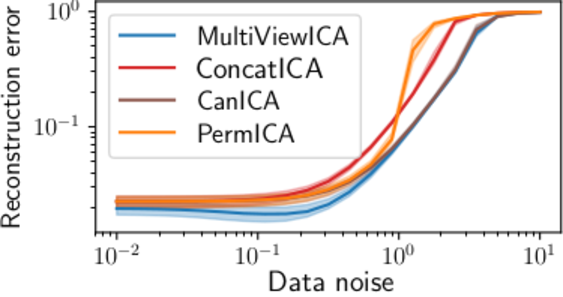
\includegraphics[width=0.38\textwidth]{figures/mvica/distance_expe.pdf}
\captionof{figure}{\textbf{Synthetic experiment}: reconstruction error of the algorithms on data following model~\eqref{eq:mvica:model}.}
\end{wrapfigure}

\textbf{Synthetic experiment}
We validate our method on synthetic data generated according to the model in equation~\eqref{eq:mvica:model}.
%
The components are generated i.i.d. from a Laplace density $d(x)=\frac12\exp(-|x|)$.
%
The mixing matrices $A_1,\cdots, A_m$ are generated with i.i.d. entries following a normal law.
Each compared algorithm returns a sequence of estimated unmixing matrices $W_1, \dots, W_m$.
%
The performance of an algorithm is measured by the reconstruction error between the estimated components and the true components.
%$\frac1M\sum_{i=1}^Md(W_iA_i)$, where $d(P)=\sum_{i=1}^n \left(\sum_{j=1}^n\frac{|p_{ij}|}{\max_{k} |p_{ik}|} - 1\right) + \sum_{j=1}^n \left(\sum_{i=1}^n\frac{|p_{ij}|}{\max_{k} |p_{kj}|} - 1\right)$.
%
%This quantity cancels if and only if $P$ is a scale and permutation matrix.
%
We use $m=10$ datasets, $k=15$ components and $n=1000$ samples. Each experiment is repeated with $100$ random seeds.
%
We vary the noise level in the data generation from $10^{-2}$ to $10$.

Multiview ICA has uniformly better performance than the other algorithms, which illustrates the strength of maximum-likelihood based methods. In accordance with results of section~\ref{sec:mvica}, it is able to separate the components even with misspecified noise parameter and components density.
%
%\subsection{fMRI experiments}
%\label{sec:experiments}

\textbf{fMRI data and preprocessing} 
We evaluate the performance of our approach on four different fMRI datasets.
%
The \emph{sherlock} dataset~\cite{chen2017shared} contains recordings of 16 subjects watching an episode of the BBC TV show "Sherlock" (50 mins).
%
The \emph{forrest} dataset~\cite{hanke2014high} was collected while 19 subjects were listening to an auditory version of the film "Forrest Gump" (110 mins).
%
The \emph{clips} dataset~\cite{ibc} was collected while 12 participants were exposed to short video clips (130 mins).
%
The \emph{raiders} dataset~\cite{ibc} was collected while 11 participants were watching the movie "Raiders of the Lost Ark" (110 mins).
%
The \emph{raiders-full} dataset~\cite{ibc} is an extension of the \emph{raiders} dataset where the first two scenes of the movie are shown twice (130 mins).
%
Like \cite{zhang2016searchlight}, we used full brain data. The rest of the preprocessing is identical to \cite{chen2017shared}. See \ref{preprocessing} for a detailed description of the datasets and preprocessing steps. Unless stated otherwise we use spatially unsmoothed data, except for the \emph{sherlock} dataset, for which the available data are already preprocessed with a 6\,mm spatial smoothing. All datasets are built from successive acquisitions called \emph{runs} that typically last 10 minutes each.
%
We define the chance level as the performance of an algorithm that computes unmixing matrices and projections to lower dimensional space by sampling random numbers from a standard normal distribution. 
%

\textbf{Reconstructing the BOLD signal of missing subjects}
We want to show that once unmixing matrices have been learned, they can be
used to predict
evoked responses across subjects, which can be useful to perform transfer learning~\cite{zhang2018transfer}.
%
We split the data into three groups. First, we randomly choose $80\%$ of all runs from all subjects to form the training set.
%
Then, we randomly choose $80\%$ of subjects and take the remaining $20\%$  runs as testing set.
%
The left-out runs  of the remaining $20\%$ subjects form the validation set.
%
The compared algorithms are run on the training set and evaluated using the testing and validation sets.
%
After an algorithm is run on training data, it defines for each subject a \emph{forward operator} that maps individual data to the components space and a \emph{backward operator} that maps the components space to individual data. For instance in ICA the forward operator is the product of the dimensionality reduction projection and unmixing matrix.
%
We estimate the shared responses on the testing set by applying the forward operators on the testing data and averaging. Finally, we reconstruct the individual data from subjects in the validation set by applying the backward operators to the shared responses. We measure the difference between the true signal and the reconstructed one using voxel-wise $R^2$ score. The $R^2$ score between two series $\xb \in \bbR^n$ and $\yb \in \bbR^n$ is defined as
$R^2(\xb, \yb) = 1 - \frac1{n\Var(\yb)}\sum_{t=1}^n (x_t - y_t)^2$, where $\Var(\yb) = \frac1n\sum_{t=1}^n (y_t - \frac1n \sum_{t'=1}^n y_{t'})^2$ is the empirical variance of $\yb$.
%
The $R^2$ score is always smaller than $1$, and equals $1$ when $\xb= \yb$.
The experiment is repeated 25 times with random splits to obtain error bars.


In this experiment we apply a 6\,mm spatial smoothing to all datasets. The $R^2$ score per
voxel depends heavily on which voxel is considered. For example voxels in the
visual cortex are better reconstructed in the \emph{sherlock} dataset than in
the \emph{forrest} dataset (see Figure~\ref{fig:brainmaps} in appendix~\ref{brainmaps}). In Figure~\ref{fig:reconstruction}
(top) we plot the mean $R^2$ score inside a region of interest (ROI) in order to leave out regions where there is no useful information.
%
ROIs are chosen based on the performance of GroupICA (more
details in appendix~\ref{brainmaps}).
%
MultiView ICA has similar or better performance than the other methods on all datasets.
%
This demonstrates its ability to capture inter-subject variability, making it a candidate of choice to handle missing data or perform transfer learning.

\textbf{Between subjects time-segment matching} 
We reproduce the time-segment matching experiment of
\cite{chen2015reduced}. 
We split the runs into a train and test set. After fitting the model on the training set, we apply the forward operator of each subject on the test set yielding individual components matrices. We estimate the shared responses by averaging the individual components of each subjects but one.  We select a target time-segment (9 consecutive timeframes) in the shared responses and try to localize the corresponding time segment in the components of the left-out subject using a maximum-correlation classifier.
This is a standard evaluation of SRM-like methods also used in  \cite{chen2015reduced}, \cite{guntupalli2018computational}, \cite{Nastase741975} or
\cite{zhang2016searchlight}.
%
The time-segment is said to be
correctly classified if the correlation between the sample and target
time-segment is higher than with any other time-segment (partially overlapping time windows are excluded).
%
We use 5-Fold cross-validation across runs: the training set contains 80\% of the runs and the test set 20\%, and repeat the experiment using all possible choices for left-out subjects. 
%
The mean accuracy is reported in Figure~\ref{exp:timesegment} (bottom). 
%
MultiView ICA yields a consistent and substantial improvement in accuracy compared to other methods on the four datasets. We see a marked improvement on the datasets sherlock and forrest. A possible explanation lies in the preprocessing pipeline. Sherlock data undergo a 6~mm spatial smoothing and Forrest data are acquired at a higher resolution (7T vs 3T for other data). This affects the signal to noise ratio.
%
In appendix~\ref{sec:app_sigma_impact}, we compute the accuracy of MultiviewICA on the sherlock dataset with 10 components when the noise parameter varies. MultiviewICA performs consistently well for a wide range of noise parameter values, and only breaks at very high values. It supports the theoretical claim of Prop~\ref{prop:robust} that the noise parameter is of little importance.

In appendix~\ref{app_spatialmaps}, we present a variation of this experiment.  We measure the ability of each algorithm to extract meaningful shared components that correlate more when they correspond to the same stimulus than when they correspond to distinct stimuli and show the improved performance of MultiView ICA. 
%
In appendix~\ref{sec:spatial_maps}, we plot the average forward operator across subjects of MultiView ICA and GroupICA with 5 components on the forrest, sherlock, raiders and clips datasets.

%\subsection{MEG experiments}
\textbf{Phantom MEG data}
We demonstrate the usefulness of our approach on MEG data.
%
The first experiment uses data collected with a realistic head phantom, which is a plastic device mimicking real electrical brain components.
%
Eight current dipoles positioned at different locations can be switched on or off.
%
We view each dipole as a subject and therefore have $m=8$.
%
We only consider the 102 magnetometers.
%
An epoch corresponds to 3\,s of MEG signals where a dipole is switched on for 0.4\,s with an oscillation at 20\,Hz and a peak-to-peak amplitude of 200\,nAm.
%
This yields a matrix of size $p\times n$ where $p=102$ is the number of sensors, and $n$ is the number of time samples.
%
We have access to $100$ epochs per dipole.
%
For each dipole, we chose $N_e=2, \dots, 16$ epochs at random among our set of 100 epochs and concatenate them in the temporal dimension.
%
We then apply algorithms on these data to extract $k=20$ shared components.
%
As we know the true components (the timecourse of the dipole), we can compute the reconstruction error of each components as the squared norm of the difference between the estimated components and the true components, after normalization to unit variance and fixing the sign.
%
We only retain the components of minimal error.
%
We also estimate for each forward operator the localization of the components by performing dipole fitting using its column corresponding to the components of minimal error.
%
We then compute the distance of the estimated dipole to the true dipole.
%
These metrics are reported in figure~\ref{fig:meg} when the number of epochs considered $N_e$ varies.
%
We also compare our method to the Bayesian Canonical Correlation Analysis (BCorrCA) of~\cite{kamronn2015multiview}.
%
On this task, BCorrCA is outperformed by ICA methods.
%
MultiView ICA requires fewer epochs to correctly reconstruct and localize the true components.
%

\textbf{Experiment on Cam-CAN dataset}
Finally, we apply MultiView ICA on the Cam-CAN dataset~\cite{taylor2017cambridge}. We use the magnetometer data from the MEG of $200$ subjects.
%
Each subject is repeatedly presented an audio-visual stimulus. 
%
The MEG signal corresponding to these trials are then time-averaged to isolate the evoked response, yielding individual data.
%
The MultiView ICA algorithm is then applied to extract $20$ shared components.
%
$9$ components were found to correspond to noise by visual inspection, and the $11$ remaining are displayed in figure~\ref{fig:meg}.
%
We observe that MultiView ICA recovers a very clean sequence of evoked potentials with sharp peaks
for early components and slower responses for late components.
%
In order to visualize their localization, we perform components localization for each subject by solving the inverse problem using sLORETA~\cite{pascual2002standardized}, providing a components estimate for each components.
%
Then, we register each components estimate to a common reference brain.
%
Finally, the components estimates are averaged, and thresholded maps are displayed in figure~\ref{fig:meg}.
%
Individual maps corresponding to each components are displayed in appendix~\ref{sec:app_montages}.
The figure highlights both early auditory and visual cortices, also suggesting a propagation
of the activity towards the ventral regions and higher level visual areas.

\begin{figure}
    \centering
    \begin{minipage}{\linewidth}
      \begin{minipage}{0.55\linewidth}
        \begin{subfigure}{\textwidth}
            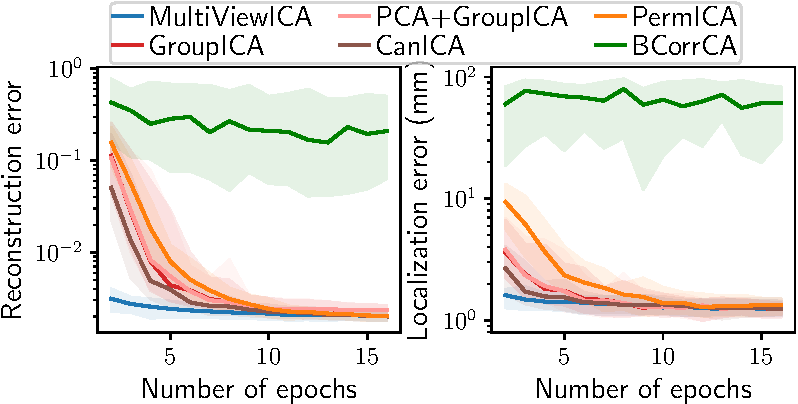
\includegraphics[width=0.99\linewidth]{figures/mvica/phantom_new.pdf}
            \caption{Phantom experiment} %{Light Unit}
        \end{subfigure}
      \end{minipage}
      \hfill
      \begin{minipage}{0.45\linewidth}
        \begin{subfigure}[t]{\textwidth}
            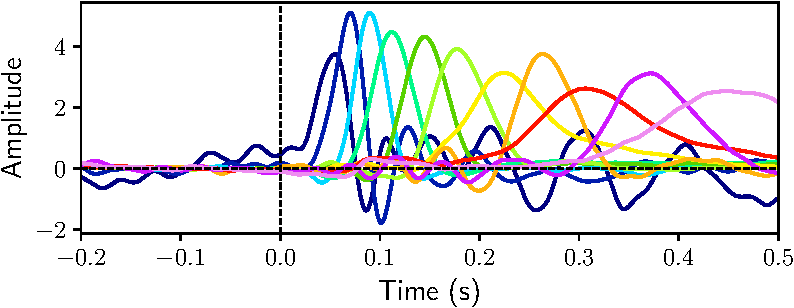
\includegraphics[width=0.99\textwidth]{figures/mvica/camcan_sources.pdf}
        \end{subfigure}\\
        \begin{subfigure}[t]{\textwidth}
            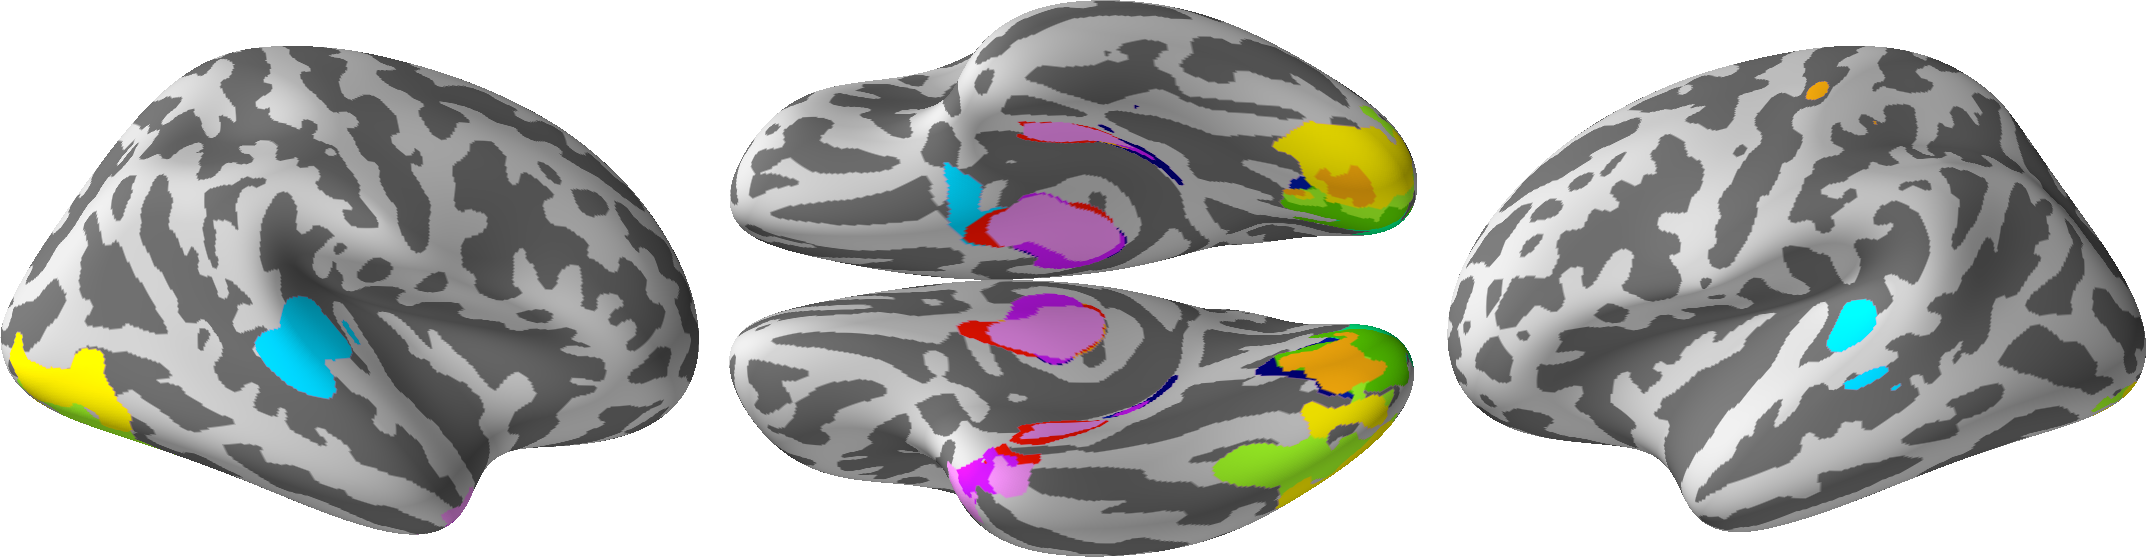
\includegraphics[width=0.99\textwidth]{figures/mvica/montage_all.png}
            \caption{Cam-CAN experiment}
        \end{subfigure}
      \end{minipage}
    \end{minipage}
    \setlength{\belowcaptionskip}{-10pt}
    \caption{\emph{Left:} \textbf{Experiment on MEG Phantom data}. Reconstruction error is the norm of the difference between the estimated and true components. Localization error is the distance between the estimated and true dipole. \emph{Right:} \textbf{Experiment on 200 subjects from the CAM-can dataset} \emph{Top:} Time course of $11$ shared components (one color per components). We recover clean evoked potentials. \emph{Bottom:} Associated brain maps, obtained by averaging components estimates registered to a common reference.}
    \label{fig:meg}
\end{figure}

\vspace{-11pt}
%
%
% \section{Conclusion}
% \label{sec:disc}
% We have proposed a novel unsupervised algorithm that reveals latent components
% observed through different views. Using an independence assumption, 
% we have demonstrated that the model is identifiable.
% %
% In contrast to previous approaches, the proposed model leads to a closed-form likelihood, which we then optimize efficiently using a dedicated alternate quasi-Newton approach.
% %
% Our approach enjoys the statistical guarantees of maximum-likelihood theory, while still being tractable.
% %
% We demonstrated the usefulness of MultiView ICA for neuroimaging group studies both on fMRI and MEG data, where it outperforms other methods.
% %
% In the experiments on fMRI data, we used temporal ICA in order to make use of the fact that subjects were exposed to the same stimuli. However, applying MultiViewICA on transposed data would carry out spatial ICA. Therefore MultiViewICA can be readily used to analyse different kind of neuroimaging data such as resting state data. 
% %
% Our method is not specific to neuroimaging data and could be relevant to other observational sciences like genomics or astrophysics where ICA is already widely used.
% %
% %
% %\section{Conclusions}
% %\label{sec:conclusions}
% %We propose a new method for modeling shared responses in neuroimaging studies. The method is identifiable and, overall, it rocks.
% %
% %
% % \section*{References}

% \subsection{Optimization}
% \subsection{Properties}
% \subsubsection{Identifiability}
% \subsubsection{Robustness to density missmatch}
% \subsubsection{A stability criterion}

\chapter{Shared ICA (ShICA)}
\section{Introduction}
In many data science problems, data are available through different views. In general, views represent different measurement modalities such as audio and video, or the same text can be available in different languages. Our main interest here is neuroimaging where recordings are made from several subjects. In particular, it is of interest to find common patterns or responses that are shared between subjects when they receive the same stimulation or perform the same cognitive task \citep{chen2015reduced,richard2020modeling}. 

A popular line of work to perform such shared response modeling is given by group independent component analysis (ICA) methods. The fastest methods~\cite{calhoun2001method, varoquaux2009canica} are among the most popular, yet they are not grounded on principled probabilistic models for the multiview setting. 
%
More principled approaches exist~\cite{richard2020modeling, guo2008unified}, however they do not model subject specific-deviations from the shared response; the magnitude of the response may differ across subjects \cite{penny2007random}, as does any noise due to heart beats, respiratory artefacts or head movement~\cite{liu2016noise}.
%
More importantly, most GroupICA methods are typically unable to separate Gaussian components.

Independent vector analysis (IVA)~\cite{lee2008independent, anderson2011joint} suggests a powerful framework, where components are independent within views but each component of a given view can depend on the corresponding component in other views. 
%
However, the two most common implementations (IVA-L~\cite{lee2008independent} and IVA-G~\cite{anderson2011joint}) only estimate view-specific components, and do not model or extract a shared response. 
%\bt{What versions of IVA ? need to be more precise}
%
They are thus not well-suited for modelling the dependencies between views in functional brain imaging, as we will argue in detail below. On the other hand, the shared response model~\cite{chen2015reduced} is a popular approach to perform shared response modeling, yet it imposes orthogonality constrains that are too restrictive and not biologically plausible.

In this work we introduce Shared ICA (ShICA), where each dataset is modeled as a linear transform of shared independent components contaminated by additive Gaussian noise. ShICA allows for principled extraction of the shared components (or responses) in addition to view-specific components. 
%
Since it incorporates a statistically sound noise model, it enables optimal inference (minimum mean squared error, MMSE) of the shared responses.
%, as well as the parameters modelling individual differences.
% \ag{last sentence can be improved}

The paper is organized as follows.
We first analyse the theoretical properties of the ShICA model, before providing powerful inference algorithms.
First, we exhibit necessary and sufficient conditions for ShICA to be identifiable (previous work only shows local identifiability~\cite{anderson2014independent}), in the presence of Gaussian or non-Gaussian components. 
%
We then introduce an algorithm called ShICA-J that uses Multiset CCA to fit the model when all the components are assumed to be Gaussian. We exhibit necessary and sufficient conditions for Multiset CCA to be able to fit the model (previous work only gives sufficient conditions~\cite{li2009joint}) and provide examples on which ShICA-J can recover the mixing matrices, while Multiset CCA cannot. 
%
We next point out a practical problem, namely that even a small sampling noise can lead to large rotations of unmixing matrices when Multiset CCA is used. To address this issue and recover the correct unmixing matrices, we propose to apply joint diagonalization to the result of Multiset CCA.
%
We further introduce ShICA-ML, a maximum likelihood estimator of ShICA that models non-Gaussian components using a Gaussian mixture model. 
%
While ShICA-ML yields more accurate components, ShICA-J is significantly faster and offers a great initialization to ShICA-ML.
Experiments on fMRI and MEG data demonstrate that the ensuing method outperforms existing GroupICA and IVA methods.


\section{Shared ICA (ShICA): an identifiable multi-view model}
\paragraph{Notations} We write vectors in bold letter $\vb$ and scalars in lower case $a$. Upper case letters $M$ are used to denote
matrices. We denote $|W|$ the absolute value of the determinant of $W$. $\xb \sim \Ncal(\mub, \Sigma)$ means that $\xb \in \mathbb{R}^k$ follows
a multivariate normal distribution of mean $\mub \in \mathbb{R}^k$ and
covariance $\Sigma \in \mathbb{R}^{k \times k}$. The $j, j$ entry of a diagonal matrix $\Sigma_i$ is denoted $\Sigma_{ij}$, the $j$ entry of $\yb_i$ is denoted $y_{ij}$. Lastly, $\delta$ is the Kronecker delta.

\paragraph{Model Definition} In the following, $\xb_1, \dots ,\xb_m \in \bbR^p$ denote the $m$ observed random vectors obtained from the $m$ different views. We posit the following generative model, called Shared ICA (ShICA): for $i= 1\dots m$
\begin{equation}
  \label{eq:model}
   \xb_i = A_i(\sbb + \nb_i)
\end{equation}
where $\sbb \in \mathbb{R}^{p}$ contains the latent variables giving the \emph{shared components}, $A_1,\dots, A_m\in\bbR^{p\times p}$ are invertible mixing matrices, and $\nb_i \in
\mathbb{R}^{p}$ are \emph{individual noises}. The individual noises model both the deviations of a view  from the mean ---i.e.\ individual differences--- and measurement noise. Importantly, we explicitly model both the shared components and the individual differences in a probabilistic framework to enable an optimal inference of the parameters and the responses.

We assume that the shared components are statistically independent, and that the individual noises are Gaussian and independent from the shared components:
$p(\sbb) = \prod_{j=1}^p p(s_j)$ and $\nb_i \sim\mathcal{N}(0, \Sigma_i)$, where the matrices $\Sigma_i$ are assumed diagonal and positive. Without loss of generality, components are assumed to have unit variance $\bbE[\sbb \sbb^{\top}] = I_p$. We further assume that there are at least 3 views: $m \geq 3$. 

In contrast to almost all existing works, we assume that some components (possibly all of them) may be Gaussian, and denote $\mathcal{G}$ the set of Gaussian components: $\sbb_j \sim \mathcal{N}(0, 1)$ for $j \in \mathcal{G}$. The other components are non-Gaussian: for $j\notin \mathcal{G}$, $\sbb_j$ is non-Gaussian.
%We denote $g$ the number of Gaussian components.


\paragraph{Identifiability} The parameters of the model are $\Theta = (A_1, \dots, A_m, \Sigma_1, \dots, \Sigma_m)$. We are interested in the identifiability of this model: given observations $\xb_1,\dots, \xb_m$ generated with parameters $\Theta$, are there some other $\Theta'$ that can generate the same observations?
Let us consider the following assumption that requires that the individual noises for Gaussian components are sufficiently diverse:
%
\begin{assumption}[Noise diversity in Gaussian components]
\label{ass:diversity}
For all $j, j' \in \mathcal{G}, j \neq j'$, the sequences $(\Sigma_{ij})_{i=1 \dots m}$ and $(\Sigma_{ij'})_{i=1 \dots m}$ are different where $\Sigma_{ij}$ is the $j, j$ entry of $\Sigma_i$
\end{assumption}

It is readily seen that there is one trivial set of indeterminacies in the problem: if $P \in \mathbb{R}^{p \times p}$ is a sign and permutation matrix the parameters $(A_1 P, \dots, A_m P, P^{\top}\Sigma_1 P, \dots, P^{\top} \Sigma_m P)$ also generate $\xb_1,\dots, \xb_m$. The following theorem shows that under the above assumption, these are the only indeterminacies of the problem.

\begin{theorem}[Identifiability]
\label{thm:identif}
We suppose Assumption~\ref{ass:diversity}. We let $\Theta'=(A_1', \dots, A_m', \Sigma_1', \dots,\Sigma_m')$ another set of parameters, and assume that they also generate $\xb_1,\dots, \xb_m$. Then, there exists a sign and permutation matrix $P$ such that for all $i$, $A_i'=A_iP$, and $\Sigma_i'= P^{\top} \Sigma_i P$.
\end{theorem}
The proof is in Appendix~\ref{proof:identif}. Identifiability in the Gaussian case is a consequence of the identifiability results in~\cite{via2011joint} and in the general case, local identifiability results can be derived from the work of ~\cite{anderson2014independent}. 
%
However local identifiability only shows that for a given set of parameters there exists a neighborhood in which no other set of parameters can generate the same observations~\cite{rothenberg1971identification}. In contrast, the proof of Theorem~\ref{thm:identif} shows global identifiability.

% \pierre{Lacks biblio: this result is not from us per se}
Theorem~\ref{thm:identif} shows that the task of recovering the parameters from the observations is a well-posed problem, under the sufficient condition of Assumption~\ref{ass:diversity}.  We also note that Assumption~\ref{ass:diversity} is necessary for identifiability. For instance, if $j$ and $j'$ are two Gaussian components such that $\Sigma_{ij} = \Sigma_{ij'}$ for all $i$, then a global rotation of the components $j, j'$ yields the same covariance matrices. The current work assumes $m \geq 3$, in appendix~\ref{app:identifiability} we give an identifiability result for $m=2$.



\section{Estimation of components with noise diversity via joint-diagonalization}

We now consider the computational problem of efficient parameter inference. This section considers components with noise diversity, while the next section deals with non-Gaussian components.


\subsection{Fitting ShICA via Multiset CCA}
If we assume that the components are all Gaussian, % \aapo{[Aapo: move to section 3.1?]}
the covariance of the observations given by
$C_{ij}=  \bbE[\xb_i\xb_j^\top] = A_i(I_p + \delta_{ij}\Sigma_i)A_j^{\top}\enspace
$ are sufficient statistics and methods using only second order information, like Multiset CCA, are candidates to estimate the parameters of the model.
Consider the
matrix $C \in \bbR^{pm \times pm}$ containing $m \times m$ blocks of size $p
\times p$
such that the block $i,j$ is given by $C_{ij}$. Consider the matrix $D$ identical to $C$ excepts that the non-diagonal blocks are filled with zeros. 
Generalized CCA consists in the following generalized eigenvalue problem:
\begin{equation}
\label{eq:eigv}
    C \ub = \lambda D\ub,\enspace \lambda > 0,\enspace \ub\in\bbR^{pm} \enspace .
\end{equation}
  
Consider the matrix $U = [\ub^1, \dots, \ub^p] \in \mathbb{R}^{mp \times p}$ formed by concatenating the $p$ leading eigenvectors of the previous problem ranked in decreasing eigenvalue order. Then, consider $U$ to be formed of $m$ blocks of size $p \times p$ stacked vertically and define $(W_i)^{\top}$ to be the $i$-th block. These $m$ matrices are the output of Multiset CCA. We also denote $\lambda_1 \geq \dots \geq \lambda_p$ the $p$ leading eigenvalues of the problem.
  %\aapo{[Very difficultto understand! First define the matrix by u's, and then say that you take blocks out of it to define the W.]}

An application of the results of \cite{li2009joint} shows that Multiset CCA recovers the mixing matrices of ShICA under some assumptions.
%
\begin{proposition}[Sufficient condition for solving ShICA via Multiset CCA~\cite{li2009joint}]
Let $r_{ijk} = (1 + \Sigma_{ik})^{-\frac12} (1 + \Sigma_{jk})^{-\frac12}$.
%\bt{Hm. What is $\Sigma_{ik}$ ?}
Assume that $(r_{ijk})_k$ is non-increasing. Assume that the maximum eigenvalue $\nu_k$ of matrix $R^{(k)}$ of general element $(r_{ijk})_{ij}$ is such that  $\nu_k = \lambda_k$ 
%\bt{$\nu_k$ is not defined}
.
Assume that $\lambda_1 \dots \lambda_p$ are distinct.
Then, there exists scale matrices $\Gamma_i$ such that $W_i = 
\Gamma_i A_i^{-1}$ for all $i$.
\end{proposition}
This proposition gives a sufficient condition for solving ShICA with Multiset CCA. It needs a particular structure for the noise covariances as well as specific ordering for the eigenvalues. The next theorem shows that we only need $\lambda_1 \dots \lambda_p$ to be distinct for Multiset CCA to solve ShICA:
\begin{assumption}[Unique eigenvectors]
  \label{ass:uniqueeig}
$\lambda_1 \dots \lambda_p$ are distinct.
\end{assumption}
% \pierre{talk a bit about these assumptions and the eigenvalue distribution}
\begin{theorem}
  \label{th:eig}
  We suppose
  Assumption~\ref{ass:uniqueeig} (only). Then, there exists a permutation matrix $P$ and scale matrices $\Gamma_i$ such that $W_i = P\Gamma_i A_i^{-1}$ for all $i$.
\end{theorem}
The proof is in Appendix~\ref{proof:eig}. This theorem means that solving the generalized eigenvalue problem~\eqref{eq:eigv} allows to recover the mixing matrices up to a scaling and permutation: this form of generalized CCA recovers the parameters of the statistical model.
Note that Assumption~\ref{ass:uniqueeig} is also a necessary condition. Indeed, if two eigenvalues are identical, the eigenvalue problem is not uniquely determined.

%\aapo{[Aapo: due to lack of space the rest of this subsection could be moved to suppl material.]}
We have two different Assumptions, \ref{ass:diversity} and \ref{ass:uniqueeig}, the first of which guarantees theoretical identifiability as per Theorem~\ref{thm:identif} and the second guarantees consistent estimation by Multiset CCA as per Theorem~\ref{th:eig}. Next we will discuss their connections, and show some limitations of the Multiset CCA approach. To begin with, we have the following result about the eigenvalues of the problem~\eqref{eq:eigv} and the $\Sigma_{ij}$.
% \pierre{best not to use a pointer to the appendix in the text, just state the following result}
\begin{prop}
  \label{prop:eigvals_from_noise}
  For $j\leq p$, let $\lambda_j$ the largest solution of $ \sum_{i=1}^m\frac{1}{\lambda_j(1 + \Sigma_{ij}) -\Sigma_{ij}}=1$. Then, $\lambda_1, \dots, \lambda_p$ are the $p$ largest eigenvalues of problem~\eqref{eq:eigv}.
\end{prop}
It is easy to see that we then have $\lambda_1, \dots, \lambda_p$ greater than $1$, while the remaining eigenvalues are lower than $1$.
From this proposition, two things appear clearly. First, Assumption~\ref{ass:uniqueeig} implies Assumption~\ref{ass:diversity}.
%
Indeed, if the $\lambda_j$'s are distinct, then the sequences $(\Sigma_{ij})_i$ must also be different from the previous proposition.
%
This is expected as from Theorem~\ref{th:eig}, Assumption~\ref{ass:uniqueeig} implies identifiability, which in turn implies Assumption~\ref{ass:diversity}.
% \pierre{I wrote this but this is really pompous}

Prop.~\ref{prop:eigvals_from_noise} also allows us to derive cases where Assumption~\ref{ass:diversity} holds but not Assumption~\ref{ass:uniqueeig}. The following Proposition shows that we can chose parameters of the model so that the model is identifiable but it cannot be solved using Multiset CCA:
\begin{prop}
\label{counter}
Assume that for two integers $j, j'$, the sequence $(\Sigma_{ij})_i$ is a permutation of $(\Sigma_{ij'})_i$, i.e. that there exists a permutation of $\{1,\dots, p\}$, $\pi$, such that for all $i$, $\Sigma_{ij} = \Sigma_{\pi(i)j'}$.  Then, $\lambda_j = \lambda_{j'}$.
\end{prop}
In this setting, Assumption~\ref{ass:diversity} holds so ShICA is identifiable, while Assumption~\ref{ass:uniqueeig} does not hold, so Multiset CCA cannot recover the unmixing matrices.




\subsection{Sampling noise and improved estimation by joint diagonalization} \label{sec:samplingnoise}


The consistency theory for Multiset CCA developed above is conducted under the assumption that the
covariances $C_{ij}$ are the true covariances of the model, and not
approximations obtained from observed samples. In practice, however, a serious limitation of Multiset CCA is that even a slight error of estimation on the covariances, due to ``sampling noise'', can yield a large error in the estimation of the unmixing matrices, as will be shown next.


\begin{wrapfigure}{r}{.4\textwidth}
\vspace{-1.5em}
\centering
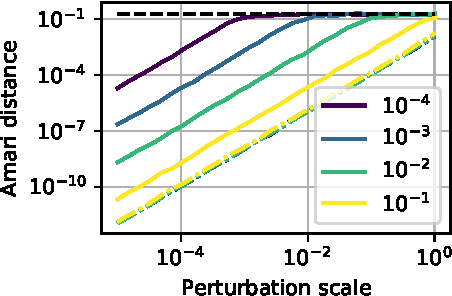
\includegraphics[width=.99\linewidth]{figures/amvica/multicca_gap_jd.pdf}
\caption{Amari distance between true mixing matrices and estimates of Multiset CCA when covariances are perturbed. Different curves correspond to different eigen-gaps. When the gap is small, a small perturbation can lead to complete mixing. Joint-diagonalization (colored dotted lines) fixes the problem.}
\label{fig:cca_gap}
\vspace{-1.5em}
\end{wrapfigure}
We begin with an empirical illustration. We take $m=3$, $p=2$, and $\Sigma_i$ such that $\lambda_1 = 2 + \varepsilon$ and $\lambda_2 =2$ for $\varepsilon > 0$.
%
In this way, we can control the \emph{eigen-gap} of the problem, $\varepsilon$.
%
%
We take $W_i$ the outputs of Multiset CCA applied to the true covariances $C_{ij}$.
%
Then, we generate a perturbation $\Delta = \delta \cdot S$, where $S$ is a random positive symmetric $pm \times pm$ matrix of norm $1$, and $\delta >0$ controls the scale of the perturbation. 
%
We take $\Delta_{ij}$ the $p\times p$ block of $\Delta$ in position $(i, j)$, and $\tilde{W}_i$ the output of Multiset CCA applied to the covariances $C_{ij} + \Delta_{ij}$.
%
We finally compute the sum of the Amari distance between the $W_i$ and $\tilde{W}_i$: the Amari distance measures how close the two matrices are, up to scale and permutation~\cite{amari1996new}.
%\Alex{add ref to paper that explicits the Amari distance}
Fig~\ref{fig:cca_gap} displays the median Amari distance over 100 random repetitions, as the perturbation scale $\delta$ increases. The different curves correspond to different values of the eigen-gap $\varepsilon$. We see clearly that the robustness of Multiset CCA critically depends on the eigen-gap, and when it is small, even a small perturbation of the input (due, for instance, to sampling noise) can lead to large estimation errors.


This problem is very general and well studied~\cite{stewart1973error}: the mapping from matrices to (generalized) eigenvectors is highly non-smooth.
%
However, the gist of our method is that the \emph{span} of the leading $p$ eigenvectors is smooth, as long as there is a large enough gap between  $\lambda_p$ and $\lambda_{p+1}$.
For our specific problem we have the following bounds, derived from Prop.~\ref{prop:eigvals_from_noise}.
\begin{prop}
  We let $\sigma_{\max} = \max_{ij}\Sigma_{ij}$ and $\sigma_{\min} = \min_{ij}\Sigma_{ij}$. Then, $\lambda_p \geq 1 + \frac{m-1}{1+\sigma_{\max}}$, while $\lambda_{p+1}\leq 1 - \frac{1}{1 + \sigma_{min}}$.
\end{prop}
As a consequence, we have $\lambda_{p} -\lambda_{p+1} \geq \frac{m-1}{1+\sigma_{\max}} + \frac{1}{1+ \sigma_{\min}}$: the gap between these eigenvalues increases with $m$, and decreases with the noise power.

\begin{wrapfigure}{l}{.45\textwidth}
\vspace{-1.em}
\begin{minipage}{.45\textwidth}
  \begin{algorithm}[H]
  \caption{ShICA-J}
  \label{algo:shicaj}
    \begin{algorithmic}
       \STATE {\bfseries Input :} Covariances $\tilde{C}_{ij} = \bbE[\xb_i\xb_j^{\top}]$
       \STATE $(\tilde{W}_i)_i \leftarrow \mathrm{MultisetCCA}((\tilde{C}_{ij})_{ij})$
       \STATE  $Q \leftarrow \mathrm{JointDiag}((\tilde{W}_i\tilde{C}_{ii}\tilde{W}_i^{\top})_i)$
       \STATE $\Gamma_{ij} \leftarrow Q\tilde{W}_i\tilde{C}_{ij}W_j^\top Q^\top$
       \STATE $(\Phi_i)_i \leftarrow \mathrm{Scaling}((\Gamma_{ij})_{ij})$
         \STATE \textbf{Return : } Unmixing matrices $(\Phi_iQ\tilde{W}_i)_i$.
        \end{algorithmic}
  \end{algorithm}
\end{minipage}
\vspace{-1em}
\end{wrapfigure}
In this setting, when the magnitude of the perturbation $\Delta$ is smaller than $\lambda_{p}-\lambda_{p+1}$, ~\cite{stewart1973error} indicates that $\mathrm{Span}([W_1, \dots, W_m]^{\top})\simeq \mathrm{Span}([\tilde{W}_1,\dots, \tilde{W}_m]^\top)$, where $[W_1, \dots, W_m]^{\top}\in\bbR^{pm\times p}$ is the vertical concatenation of the $W_i$'s.
In turn, this shows that there exists a matrix $Q\in\bbR^{p\times p}$ such that
%
%
\begin{equation}
    \label{eq:justif_jd}
    W_i \simeq Q\tilde{W}_i\enspace \text{for all} \enspace i.
\end{equation}

We propose to use joint-diagonalization to recover the matrix $Q$. Given the $\tilde{W}_i$'s, we consider the set of symmetric matrices $\tilde{K}_i = \tilde{W}_i\tilde{C}_{ii}\tilde{W}_i^{\top}$, where $\tilde{C}_{ii}$ is the contaminated covariance of $\xb_i$. Following Eq.~\eqref{eq:justif_jd}, we have $Q\tilde{K}_iQ^{\top} = W_i \tilde{C}_{ii}W_i^{\top}$, and using Theorem~\ref{th:eig}, we have $Q\tilde{K}_iQ^{\top} = P\Gamma_i A_i^{-1}\tilde{C}_{ii}A_i^{-\top}\Gamma_iP^{\top}$. Since $\tilde{C}_{ii}$ is close to $C_{ii} = A_i (I_p + \Sigma_i)A_i^\top$, the matrix $P\Gamma_i A_i^{-1}\tilde{C}_{ii}A_i^{-\top}\Gamma_iP^{\top}$ is almost diagonal.
%
In other words, the matrix $Q$ is an approximate diagonalizer of the $\tilde{K}_i$'s, and we approximate $Q$ by joint-diagonalization of the $\tilde{K}_i$'s. In Fig~\ref{fig:cca_gap}, we see that this procedure mitigates the problems of multiset-CCA, and gets uniformly better performance regardless of the eigen-gap.
%
In practice, we use a fast joint-diagonalization algorithm~\cite{ablin2018beyond} to minimize a joint-diagonalization criterion for positive symmetric matrices~\cite{pham2001joint}. The estimated unmixing matrices $U_i = Q\tilde{W}_i$ correspond to the true unmixing matrices only up to some scaling: the information that the components are of unit variance is lost.

\textbf{Scale estimation}
We form the matrices $\Gamma_{ij} = U_i\tilde{C}_{ij}U_j^\top$. In order to estimate the scalings, we solve $
\min_{(\Phi_i)} \sum_{i\neq j} \| \Phi_i \diag(\Gamma_{ij}) \Phi_j - I_p \|_F^2$
where the $\Phi_i$ are diagonal matrices.
This function is readily minimized with respect to one of the $\Phi_i$ by the formula
$\Phi_i = \frac{\sum_{j \neq i} \Phi_j \diag(Y_{ij})}{\sum_{j \neq i} \Phi_j^2 \diag(Y_{ij})^2}$ (derivations in Appendix~\ref{app:fixedpoint}). We then iterate the previous formula over $i$ until convergence.
The final estimates of the unmixing matrices are given by
$(\Phi_i U_i)_{i=1}^m$. The full procedure, called ShICA-J, is summarized in Algorithm~\ref{algo:shicaj}.

\subsection{Estimation of noise covariance and inference of shared components}

In practice, it is important to estimate noise co-variances $\Sigma_i$ in order to take advantage of the fact that some views are noisier than others. As it is well known in classical factor analysis, modelling noise variances allows the model to virtually discard variables, or subjects, that are particularly noisy. 

Using the ShICA model with Gaussian components, we derive noise covariances estimate directly from maximum likelihood. We use an expectation-maximization (EM) algorithm, which is especially fast because noise updates are in closed-form. Following derivations given in appendix~\ref{conditional_density}, the sufficient statistics in the E-step are given by 
\begin{align}
\label{mmse1}
\EE[\sbb|\xb]= \left(\sum_{i=1}^m \Sigma_i^{-1}  + I \right)^{-1}  \sum_{i=1}^m \left(\Sigma_i^{-1} \yb_i \right)
     && \VV[\sbb|\xb]= (\sum_{i=1}^m \Sigma_i^{-1}  + I)^{-1}
\end{align}
Incorporating the M-step we get the following updates that only depend on the covariance matrices:
$
\Sigma_i \leftarrow \diag(\hat{C_{ii}} - 2 \VV[\sbb | \xb]  \sum_{j=1}^m \Sigma_j^{-1} \hat{C}_{ji}  + \VV[\sbb | \xb]  \sum_{j = 1}^m \sum_{l = 1}^m \left(\Sigma_j^{-1} \hat{C}_{jl} \Sigma_l^{-1} \right) \VV[\sbb | \xb] + \VV[\sbb | \xb])
$
%We observe very fast convergence ($10$ iterations are usually enough to reach gradients $\ell_2$ norm below $10^{-4}$).

\section{ShICA-ML: Maximum likelihood for non-Gaussian components}
ShICA-J only uses second order statistics. However, the ShICA model~\eqref{eq:model} allows for non-Gaussian components. We now propose an algorithm for fitting the ShICA model that assumes non-Gaussian components so that it can separate Gaussian and non-Gaussian components.
%\aapo{[Aapo: Motivate and link to previous sections]}
We estimate the parameters by maximum likelihood. Since most non-Gaussian components in real data are super-Gaussian, we assume that the non-Gaussian components $\sbb$ have the super-Gaussian density \\ $p(s_j) = \frac12\left(\mathcal{N}( s_j; 0, \frac12) + \mathcal{N}( s_j; 0, \frac{3}{2})\right) \enspace.$

We propose to maximize the log-likelihood using a generalized
EM~\cite{neal1998view, dempster1977maximum}. Derivations are available in Appendix~\ref{app:emestep}. Like in the previous section, the E-step is in closed-form yielding the following sufficient statistics:
\begin{align}
\label{mmse2}
\EE[\sbb | \xb] = \frac{\sum_{\alpha \in \{\frac12, \frac32
    \}}\theta_{\alpha} \eb_{\alpha}}{\sum_{\alpha \in
    \{\frac12, \frac32 \}}\theta_{\alpha}}
    && 
    \VV[\sbb | \xb] = \frac{\sum_{\alpha \in \{\frac12, \frac32
    \}}\theta_{\alpha} V_{\alpha}}{\sum_{\alpha \in
    \{\frac12, \frac32 \}}\theta_{\alpha}} 
\end{align}
    where
    $\eb_{\alpha}= \left(\sum_{i=1}^m \Sigma_i^{-1}  + \frac1{\alpha}I \right)^{-1}  \sum_{i=1}^m \left(\Sigma_i^{-1} \yb_i \right)$,  $V_{\alpha} = (\sum_{i=1}^m \Sigma_i^{-1}  + \frac1{\alpha}I)^{-1}$ and $\theta_{\alpha} = \mathcal{N}((\sum_{i=1}^m \Sigma_i^{-1})^{-1} \Sigma_i^{-1} \yb_i; 0, \alpha I + (\sum_{i=1}^m \Sigma_i^{-1})^{-1})$ with $\yb_i = W_i \xb_i$.
Noise updates are in closed-form and given by:
$\Sigma_i \leftarrow  \diag((\yb_i - \EE[\sbb | \xb]) (\yb_i - \EE[\sbb | \xb])^{\top}+ \VV[\sbb | \xb])$.
However, no closed-form is available for the updates of unmixing matrices. We therefore perform quasi-Newton updates given by
$W_i \leftarrow (I - \rho (\widehat{\mathcal{H}^{W_i}})^{-1} \mathcal{G}^{W_i}) W_i$ where $\rho \in \mathbb{R}$ is chosen by backtracking line-search, 
$\widehat{\mathcal{H}^{W_i}_{a, b, c, d}} =  \delta_{ad} \delta_{bc} + \delta_{ac} \delta_{bd}\frac{(y_{ib})^2}{\Sigma_{ia}}$ is an approximation of the Hessian of the negative complete log-likelihood and $\mathcal{G}^{W_i} = -I + (\Sigma_i)^{-1}(\yb_i - \mathbb{E}[\sbb|\xb])(\yb_i)^{\top}$ is the gradient.

We alternate between computing the statistics $\mathbb{E}[\sbb|\xb]$, 
$\mathbb{V}[\sbb|\xb]$ (E-step) and updates of parameters $\Sigma_i$ and $W_i$ for $i=1 \dots m$ (M-step). Let us highlight that our EM algorithm and in particular the E-step resembles the one used in~\cite{moulines1997maximum}. However because they assume noise on the sensors and not on the components, their formula for $\EE[\sbb| \xb]$ involves a sum with $2^p$ terms whereas we have only $2$ terms. The resulting method is called ShICA-ML.

\paragraph{Minimum mean square error estimates in ShICA}
In ShICA-J as well as in ShICA-ML, we have a closed-form for the expected components given the data $\EE[\sbb | \xb]$, shown in equation~\eqref{mmse1} and~\eqref{mmse2} respectively. This provides minimum mean square error estimates of the shared components, and is an important benefit of explicitly modelling shared components in a probabilistic framework.
%\aapo{[Aapo: The formulas for Es|x should be given as numbered equations, and they should be referred to here. But this is too short to be a proper section...]}

% \section{An alternate quasi-newton algorithm for MIFA}


% We estimate the parameters of model~\eqref{model} ($W_i$ and $\Sigma_i$) via maximum likelihood.
% As shown in Appendix~\ref{likelihood_derivation}, the negative log-likelihood is given by
% \begin{align}
%   \mathcal{L} = &\sum_{i=1}^m\left(-\log|W_i| + \frac12 \log |\Sigma_i|\right) + \frac12 \log(|\sum_{i=1}^m \Sigma_i^{-1} + I|) + \frac12 (\sum_{i=1}^m \langle \yb_i | \Sigma_i^{-1} \yb_i \rangle \\&  - \frac12 \langle \left(\sum_{i=1}^m \Sigma_i^{-1} + I \right)^{-1} \sum_{i=1}^m \left(\Sigma_i^{-1} \yb_i \right) | \sum_{i=1}^m \left(\Sigma_i^{-1} \yb_i \right) \rangle)
% \end{align}

% We optimize this likelihood using expectation-maximization (EM)~\addref.

% The completed likelihood is given by
% \begin{equation}
%   p(\xb, \sbb) = p(\xb_i | \sbb) p(\sbb)=  |W_i| \Ncal(\yb_i; \sbb, \Sigma_i) \Ncal(\sbb; 0, I_k)
% \end{equation}
% Therefore the negative completed log-likelihood is a quadratic function of the
% components so only second moments of $\sbb | \xb$ are needed. It turns out that we
% can compute $\sbb | \xb$ exactly. Derivations given in appendix~\ref{conditional_density} yield:
% \begin{align}
%   &\sbb|\xb \sim \Ncal( \EE[\sbb|\xb], \VV[\sbb | \xb]) \\
%   & \text{where } \enspace \EE[\sbb|\xb]= \left(\sum_{i=1}^m \Sigma_i^{-1}  + I \right)^{-1}  \sum_{i=1}^m \left(\Sigma_i^{-1} \yb_i \right) \text{ and } \VV[\sbb|\xb]= (\sum_{i=1}^m \Sigma_i^{-1}  + I)^{-1}
% \end{align}

% The function to minimize in the M-step is therefore given by:
% \begin{align}
%   \Jcal = \sum_{i=1}^m -\log(|W_i|) +\log(|\Sigma_i|) + \frac12 \tr(\Sigma_i^{-1} \left[(\yb_i - \EE[\sbb | \xb]) (\yb_i - \EE[\sbb | \xb])^{\top}+ \VV[\sbb | \xb]\right])  
% \end{align}

% We get closed-form updates for $\Sigma_i$ given by
% \[
% \Sigma_i \leftarrow  \diag((\yb_i - \EE[\sbb | \xb]) (\yb_i - \EE[\sbb | \xb])^{\top}+ \VV[\sbb | \xb])
% \]
% Updates with respect to $W_i$ are obtained through a quasi-newton step:
% $W_i \leftarrow (I - \rho H_i G_i^{-1}) W_i$ where the relative gradient is
% given by
% $G_i = I - \Sigma_i^{-1}(\yb_i - \EE[\sbb | \xb])\yb_i^{\top}$ and while the
% true Hessian is given by $H_{i, abcd} = \delta_{a,c} \frac{y_{i, b} y_{i,
%     d}}{\Sigma_{i, a}}$, we use for increased speed, the following
% approximation: $\tilde{H}_{i, abcd} = \delta_{a, c} \delta_{b,d}
% \frac{y_{i, b}^2}{\Sigma_{i, a}}$ which is exact when the unmixed
% data are truly independent. The step-size $\rho$ is chosen by backtracking
% line-search.

% Note that the likelihood and therefore the updates only depend on the covariance
% of the data. Therefore in practice, we pre-compute the covariances $\xb_i \xb_j^{\top}$ for
% all $1 \leq i \leq m$ and $1 \leq i \leq m$ and do not use the original data
% anymore. This provide a great speed-up when the number of samples is high.


% \begin{ack}
% Use unnumbered first level headings for the acknowledgments. All acknowledgments
% go at the end of the paper before the list of references. Moreover, you are required to declare
% funding (financial activities supporting the submitted work) and competing interests (related financial activities outside the submitted work).
% More information about this disclosure can be found at: \url{https://neurips.cc/Conferences/2021/PaperInformation/FundingDisclosure}.

% Do {\bf not} include this section in the anonymized submission, only in the final paper. You can use the \texttt{ack} environment provided in the style file to autmoatically hide this section in the anonymized submission.
% \end{ack}

% \section{A generalized eigenvalue approach for MIFA}
% While maximum-likelihood approaches possess several important statistical properties that make them attractive, a major drawback is the slowness of the algorithms. 

% These method also require the likelihood to be well defined, and prevents dimension reduction without a more complicated model: for the likelihood to be well defined, we must assume that $A_i$ is square, invertible.

% If we only consider two views, the model of MIFA in equation~\eqref{model} is
% the model of probabilistic CCA~\addref but with a different noise covariance.
% Many multiview CCA methods exists~\addref. They are typically referred to as
% Multiset CCA and differ by the objective they optimize as well as the
% constraints they put on the canonical vectors~\addref. A tractable formulation is given
% by the SUMCOR~\addref objective:
% \begin{align}
%   \rho(\vb_1 \dots \vb_m) = \sum_{i=1}^m \sum_{j \neq i}^m \vb_i^{\top} C_{ij} \vb_j,  \text{ such that } \forall i, \sum_{i=1}^m\vb_i^{\top} C_{ii} \vb_i = 1
% \end{align}
% which we can write in matrix form as
% \begin{align}
%   \rho(V_1 \dots V_m) = \sum_{i=1}^m \sum_{j \neq i}^m \tr(V_i^{\top} C_{ij} V_j),  \text{ such that } \forall i, \sum_{i=1}^m V_i^{\top} C_{ii} V_i = I
% \end{align}
% for $V^i \in \mathbb{R}^{k, p}$.

% The first order conditions yield the following generalized eigenvalue problem
% \begin{align}
%   \begin{bmatrix} C_{11} & \dots & C_{1m} \\
%     \vdots & \ddots & \vdots  \\
%     C_{m1} & \dots  &C_{mm}
%   \end{bmatrix} \begin{bmatrix} V_1 \\ \vdots \\ V_m \end{bmatrix} = \begin{bmatrix} C_{11} &  & 0 \\
%      & \ddots &   \\
%     0 &   &C_{mm}
%   \end{bmatrix} \begin{bmatrix} V_1 \\ \vdots \\ V_m \end{bmatrix} \Lambda  \label{problem}
% \end{align}
% where $\Lambda \in \mathbb{R}^{kxk}$ is a matrix of Lagrange
% multipliers. The $k$ eigenvectors corresponding to the largest eigenvalues yield
% the solution up to a global rotation.

% The following lemma shows that minimizing the above objective leads to estimates
% of the true unmixing matrices up to a view specific scaling and a global rotation.
% \begin{prop}
%   \label{gev}
%   Assume that data are generated from model~\eqref{model} with mixing matrix
%   $A_i \in \mathbb{R}^{k \times k}$ and assume all subjects have distinct
%   noise covariances $\Sigma_i$. Then, in the limit of large samples $n=\infty$,
%   the $k$ first eigenvectors of the
%   generalized eigenvalue problem~\eqref{problem} are given by
%   $\begin{bmatrix} W_1^{\top} \Gamma_1 P \\ \vdots \\ W_m^{\top} \Gamma_m P \end{bmatrix}$ where
%   $\Gamma_i$ are scale matrices and $P$ is a permutation matrix.
% \end{prop}


% \begin{prop}
%   \label{finite}
%   Assume $n < \infty$ samples are generated from model~\eqref{model} with mixing matrix
%   $A_i \in \mathbb{R}^{k \times k}$ and assume all subjects have distinct
%   noise covariances $\Sigma_i$. Then, assuming the empirical covariance is close to
%   the actual covariance the $k$ first eigenvectors are given by the formula of
%   prop~\label{gev} up to a global rotation.
% \end{prop}

  

% \section{Related Work}
% ShICA combines theory and methods coming from different branches of ``component analysis''. It can be viewed as a GroupICA method, as an extension of Multiset CCA, as an Independent Vector Analysis method or, crucially, as an extension of the shared response model. In the setting studied here, ShICA improves upon all existing methods.

% \paragraph{GroupICA}
% GroupICA methods extract independent components from multiple datasets. In its original form\cite{calhoun2001method}, views are concatenated and then a PCA is applied yielding reduced data on which ICA is applied. One can also reduce the data using Multiset CCA instead of PCA, giving a method called \emph{CanICA}~\cite{varoquaux2009canica}. Other works~\cite{Esposito05NI, Hyva11NI} apply ICA separately on the datasets and attempt to match the decompositions afterwards.
% Although these works provide very fast methods, they do not rely on a well defined model like ShICA. %In contrast, the procedure in ShICA-J is based on an explicit model.
% Other GroupICA methods impose some structure on the mixing matrices such as the tensorial method of~\cite{beckmann2005tensorial} or the group tensor model in~\cite{guo2008unified} (which assumes identical mixing matrices up to a scaling) or \cite{svensen2002ica} (which assumes identical mixing matrices but different components). In ShICA the mixing matrices are only constrained to be invertible.
% Lastly, maximum-likelihood based methods exist such as \emph{MultiViewICA}~\cite{richard2020modeling} or the full model of~\cite{guo2008unified}. These methods are weaker than ShICA as they assume non-Gaussianity, the same noise covariance across views and lack a principled method for shared response inference.
% %\aapo{These methods are weaker than from ShICA as they assume non-Gaussianity, the same noise covariance across views, and lack a principles method for shared response inference. [I hope this is all correct? - Hugo:We have seen that multiview ICA can separate Gaussian components but in practice it does it quite poorly. However we could have derived a principle method for shared response inference (but that cannot take into account the fact the some views are noisier than others) ]}
% %Aapo: But our comparison here should be limited to what is actually done and said in the papers, not what the methods could be able to do with further development. Hugo: Ok agreed !

% \paragraph{Multiset CCA}
% In its basic formulation, CCA identifies a shared space between two datasets.
% The extension to more than two datasets is ambiguous, and many
% different generalized CCA methods have been proposed. \cite{kettenring1971canonical} introduces 6 objective functions that reduce to CCA when $m=2$ and \cite{nielsen2002multiset} considered 4 different possible constrains leading to 24 different formulations of Multiset CCA. The formulation used in ShICA-J is refered to in~\cite{nielsen2002multiset} as SUMCORR with constraint 4 which is one of the fastest as it reduces to solving a generalized eigenvalue problem. The fact that CCA solves a well defined probabilistic model has first been studied in~\cite{bach2005probabilistic} where it is shown that CCA is identical to multiple battery factor analysis~\cite{browne1980factor} (restricted to 2 views). This latter formulation differs from our model in that the noise is added on the sensors and not on the components which makes the model unidentifiable. Identifiable variants and
% generalizations can be obtained by imposing sparsity on the mixing matrices such as in~\cite{archambeau2008sparse, klami2014group, witten2009extensions} or non-negativity~\cite{DELEUS2011143}.
% The work in~\cite{li2009joint} exhibits a set of sufficient (but not necessary) conditions under which a well defined model can be learnt by the formulation of Multiset CCA used in ShICA-J. The set of conditions we exhibit in this work are necessary and sufficient. We further emphasize that basic Multiset CCA provides a poor estimator as explained in Section~\ref{sec:samplingnoise}.

% \paragraph{Independent vector analysis}
% Independent vector analysis~\cite{lee2008independent} (IVA) models the data as a linear mixture of independent components $\xb_i = A_i \sbb_i$ where each component $s_{ij}$ of a given view $i$ can depend on the corresponding component in other views ($(s_{ij})_{i=1}^m$ are not independent).
% % the components $\sbb_i \in \bbR^{p}$ differ across subjects but component $j$  \bt{the joint distribution of s samples ? it is unclear what j stands for} is not independent across subjects
% Practical implementations of this very general idea assume a distribution for $p((s_{ij})_{i=1}^m)$. In IVA-L~\cite{lee2008independent}, $p((s_{ij})_{i=1}^m) \propto \exp(-\sqrt{\sum_i (s_{ij})^2})$ (so the variance of each component in each view is assumed to be the same), in IVA-G~\cite{anderson2011joint} or in~\cite{via2011maximum}, $p((s_{ij})_{i=1}^m) \sim \mathcal{N}(0, R_{ss})$ and~\cite{engberg2016independent} proposed a normal inverse-Gamma density. The model of ShICA can be seen as an instance of IVA %(where $p$ in ShICA-ML is a Gaussian mixture in which variances are learnt), 
% which specifically enables extraction of shared components from the subject specific components, unlike previous versions of IVA. In fact, ShICA comes with minimum mean square error estimates for the shared components
% %(given by $\bbE[\sbb | \xb]$) 
% that is often the quantity of interest. By contrast, the model in IVA-L has components that are uncorrelated over views, which is quite unrealistic for fMRI or any MEG/EEG evoked response, while our model is explicitly constructed to be realistic for brain imaging applications.
% The IVA theory provides global identifiability conditions in the Gaussian case (IVA-G)~\cite{via2011joint} and local identifiability conditions in the general case~\cite{anderson2014independent} from which local identifiability conditions of ShICA could be derived. However, in this work, we provide global identifiability conditions for ShICA.
% Lastly, IVA can be performed using joint diagonalization of cross covariances~\cite{li2011joint, congedo2012orthogonal} although multiple matrices have to be learnt and cross-covariances are not necessarily symmetric positive definite which makes the algorithm slower and less principled.

% \paragraph{Shared response model}
% ShICA extracts shared components from multiple datasets, which is also the goal of the shared response model (SRM)~\cite{chen2015reduced}. The robust SRM~\cite{turek2018capturing} also allows to capture subject specific noise. However these models impose orthogonality constraints on the mixing matrices while ShICA does not. Deep variants of SRM exist such as~\cite{chen2016convolutional} but while they release the orthogonality constrain, they are much more computationally demanding. ShICA leverages ICA theory to provide a much more powerful model of shared responses.

% \paragraph{Limitations}
% The main limitation of this work is that the model does not reduce the dimension inside each view. In line with other methods, such view-specific  dimension reduction has to be done by some external method, typically view-specific PCA. Using specialized methods for the estimation of covariances should also be of interest for ShICA-J, where it only relies on sample covariances. Finally, ShICA-ML uses a simple model of a super-Gaussian distribution, while modelling the non-gaussianities in more detail in ShICA-ML should improve the performance.

\section{Experiments}
Experiments used Nilearn~\cite{abraham2014machine} and MNE~\cite{gramfort2013meg} for fMRI and MEG data
processing respectively, as well as the scientific Python ecosystem:
Matplotlib~\cite{hunter2007matplotlib}, Scikit-learn~\cite{pedregosa2011scikit},
Numpy~\cite{harris2020array} and Scipy~\cite{2020SciPy-NMeth}. We use the Picard algorithm for non-Gaussian ICA~\cite{ablin2018faster}, and mvlearn for multi-view ICA~\cite{perry2020mvlearn}. The above libraries use open-source licenses. fMRI experiments used the following datasets: sherlock~\cite{chen2017shared}, forrest~\cite{hanke2014high} , raiders~\cite{ibc} and gallant~\cite{ibc}. The data we use do not contain offensive content or identifiable information and consent was obtained before data collection. Computations were run on a large server using up to 100 GB of RAM and 20 CPUs in parallel.
%\pierre{need to mention algos used+ cite}
%\Alex{I would consider replacing subsections in experiments by paragraphs to gain some space}
%
In the following synthetic experiments, data are generated according to model~\eqref{eq:model} with $p=4$ components and $m=5$ views and mixing matrices are generated by sampling coefficients from a standardized Gaussian.
\paragraph{Separation performance}
\label{sec:rotation}
%\pierre{Make sure that algos are always in the same order in legend, and that shica-j and shica ml are together}
Gaussian components are generated from a standardized Gaussian and their noise has standard deviation $\Sigma_i^{\frac12}$ (obtained by sampling from a uniform density between $0$ and $1$) while non-Gaussian components are generated from a Laplace distribution and their noise standard deviations are equal. We study 3 cases where either all components are Gaussian, all components are non-Gaussian or half of the components are Gaussian and half are non-Gaussian. We vary the number of samples $n$ between $10^2$ and $10^5$ and display in Fig~\ref{exp:rotation} the mean Amari distance across subjects as a function of $n$. The experiment is repeated $100$ times using different seeds. We report the median result and error bars  represent the first and last deciles.
\begin{figure}
\centering
  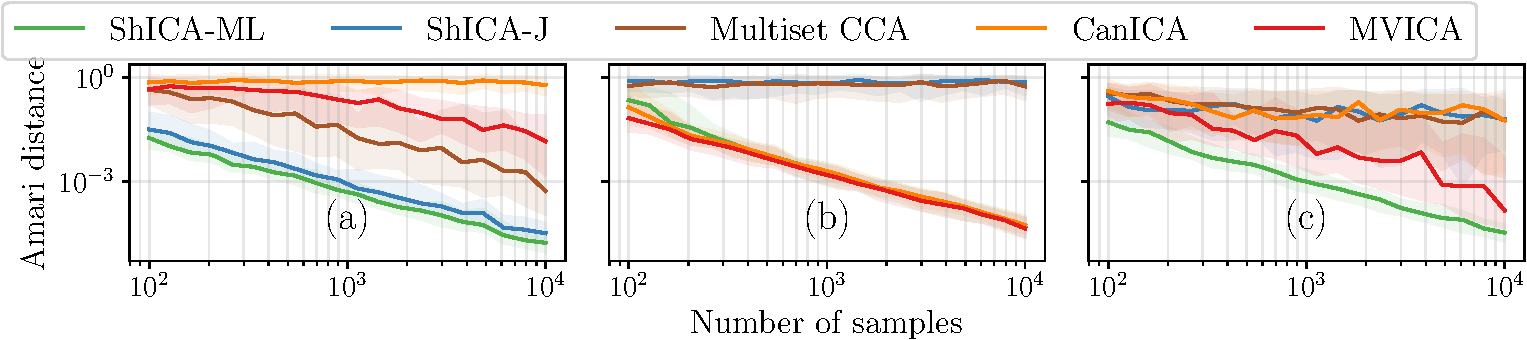
\includegraphics[width=0.9\textwidth]{./figures/amvica/identifiability.pdf}
  \vspace{-1em}
  \caption{\textbf{Separation performance}: Algorithms are fit on data following model~\ref{eq:model} \textbf{(a)} Gaussian components with noise diversity \textbf{(b)} Non-Gaussian components without noise diversity \textbf{(c)} Half of the components are Gaussian with noise diversity, the other half is non-Gaussian without noise diversity. 
  %\aapo{[It would be nice to have labels a,b,c but this is not critical.]}
  %\Alex{Make the legend fit on one line and rename Multiset CCA to Multiset CCA to be consistent with the text (or update text). Also you should be able to reduce a tiny bit the height of the axes plots.}
  }
  \label{exp:rotation}
  \vspace{-1.5em}
\end{figure}
When all components are Gaussian (Fig.~\ref{exp:rotation}~(a)), CanICA cannot separate the components at all. In contrast ShICA-J, ShICA-ML and Multiset CCA are able to separate them, but Multiset CCA needs many more samples to reach the same Amari distance as ShICA-J or ShICA-ML, which shows that correcting for the rotation due to sampling noise improves the results. Looking at error bars, we also see that the performance of Multiset CCA varies quite a lot with the random seeds: this shows that depending on the sampling noise, the rotation can be very different from identity.
When none of the components are Gaussian (Fig.~\ref{exp:rotation}~(b)), only CanICA and ShICA-ML are able to separate the components, as other methods do not make use of non-Gaussianity.
Finally, in the hybrid case (Fig.~\ref{exp:rotation}~(c)), only ShICA-ML is able to separate the components as it is the only method that can make use of both non-Gaussianity and noise diversity. Additional experiments illustrating the separation powers of algorithms are available in Appendix~\ref{app:separation}.
%

\vspace{-1.5em}
\paragraph{Computation time}
\begin{wrapfigure}{l}{.47\textwidth}
    \centering
    \vspace{-1em}
    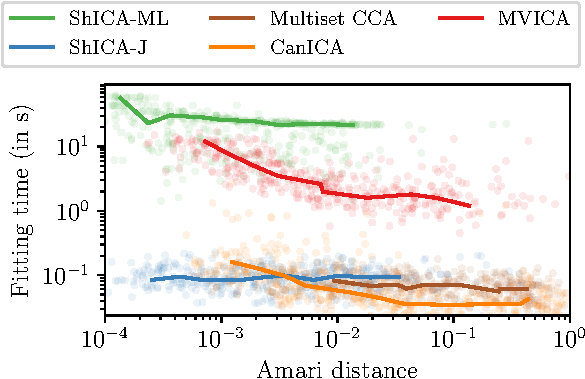
\includegraphics[width=.99\linewidth]{./figures/amvica/synthetic_gaussian_timings.pdf}
    \caption{\textbf{Computation time: } Algorithms are fit on data generated from model~\eqref{eq:model} with a super-Gaussian density. For different values of the number of samples, we plot the Amari distance and the fitting time. Thick lines link median values across seeds.}
    \label{exp:syn_timings}
\end{wrapfigure}
We generate components using a slightly super Gaussian density: $s_j = d(x)$ with $d(x) = x |x|^{0.2}$ and $x \sim \mathcal{N}(0, 1)$. We vary the number of samples $n$ between $10^2$ and $10^4$. We compute the mean Amari distance across subjects and record the computation time. The experiment is repeated $40$ times. We plot the Amari distance as a function of the computation time in Fig~\ref{exp:syn_timings}. Each point corresponds to the Amari distance/computation time for a given number of samples and a given seed. We then consider for a given number of samples, the median Amari distance and computation time across seeds and plot them in the form of a thick line.  From Fig~\ref{exp:syn_timings}, we see that ShICA-J is the method of choice when speed is a concern while ShICA-ML yields the best performance in terms of Amari distance at the cost of an increased computation time. The thick lines for ShICA-J and Multiset CCA are quasi-flat, indicating that the number of samples does not have a strong impact on the fitting time as these methods only work with covariances. On the other hand CanICA or MultiviewICA computation time is more sensitive to the number of samples.
%


%\pierre{fig might have a smaller legend: 3 cols, smaller fonts}


\paragraph{Robustness w.r.t intra-subject variability in MEG}
\begin{wrapfigure}{l}{.47\textwidth}
\vspace{-1.7em}
  \centering
  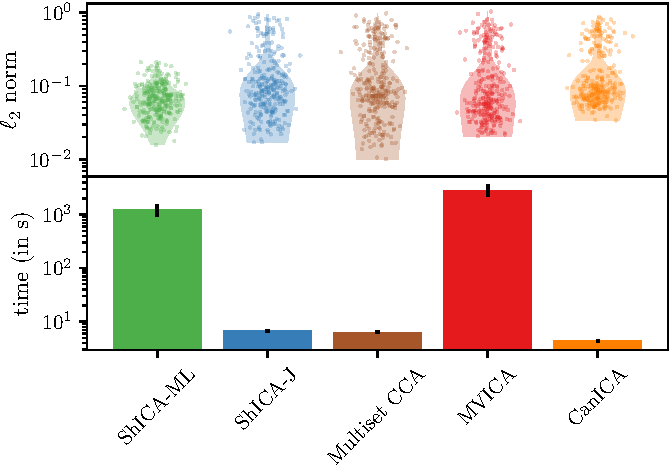
\includegraphics[width=.95\linewidth]{./figures/amvica/inter_subject_stability.pdf}
  \vspace{-0.5em}
  \caption{\textbf{Robustness w.r.t intra-subject variability in MEG}:
    (\textbf{top}) $\ell_2$ distance between shared components corresponding to the same stimuli in different trials.  (\textbf{bottom}) Fitting time.
    %\Alex{Should be $\ell_2$ in ylabel not L2}
}
\label{fig:eeg_intragroup_variability}
\vspace{-1em}
\end{wrapfigure}
In the following experiments we consider the Cam-CAN
dataset~\cite{taylor2017cambridge}. We use the magnetometer data from the MEG of $m=100$ subjects chosen randomly among 496.
% 
Each subject is repeatedly presented three audio-visual stimuli. 
% 
For each stimulus, we divide the trials into two sets and within each set, %Aapo: "sets"
the MEG signal is averaged across trials to isolate the evoked response. This
procedure yields 6 chunks of individual data (2 per stimulus).
%
% The 6 chunks of data are concatenated in the time direction and ICA algorithms
% are applied separately to extract $k=10$ shared components that we plot in
% appendix~\ref{megcomponents} and localize in appendix~\ref{megcomponentslocal}.
%
We study the similarity between shared components corresponding to repetitions of the same stimulus. This gives a measure of robustness of each ICA algorithm with respect
to intra-subject variability.
Data are first reduced using a subject-specific PCA with $p=10$ components. Algorithms are run 10 times with different seeds on the 6 chunks of data,
and shared components are extracted.
%
When two chunks of data correspond to repetitions of the same stimulus they should yield similar
components.
%
For each component and for each stimulus, we therefore measure the $\ell_2$
distance between the two repetitions of the stimulus.
 This yields $300$ distances per algorithm that are
plotted on Fig~\ref{fig:eeg_intragroup_variability}.

The components recovered by ShICA-ML have a much lower variability than other approaches. The performance of ShICA-J is competitive with Multiview ICA while being much faster to fit. Multiset CCA yields satisfying results compared with ShICA-J. However we see that the number of components that do not match at all across trials is greater in Multiset CCA.
    %\bt{Muliview ICA appears only now ?} \aapo{[Actually, multiset CCA looks just as good as ShICA-J?, comments?.]}
Additional experiments on MEG data are available in Appendix~\ref{app:phantom}.
% The difference between AVICA and other approaches can be quantified via a
% statistical t-test on the difference of log distances. It
% gives the p-values $4.57 \times 10^{-4}$, $5.93 \times 10^{-4}$ and $2.37
% \times 10^{-9}$ w.r.t.
% MVICA, PermICA and ConcatICA respectively.
\vspace{-1em}
\paragraph{Reconstructing the BOLD signal of missing subjects}
\begin{wrapfigure}{l}{.42\textwidth}
\vspace{-0.5em}
  \centering
  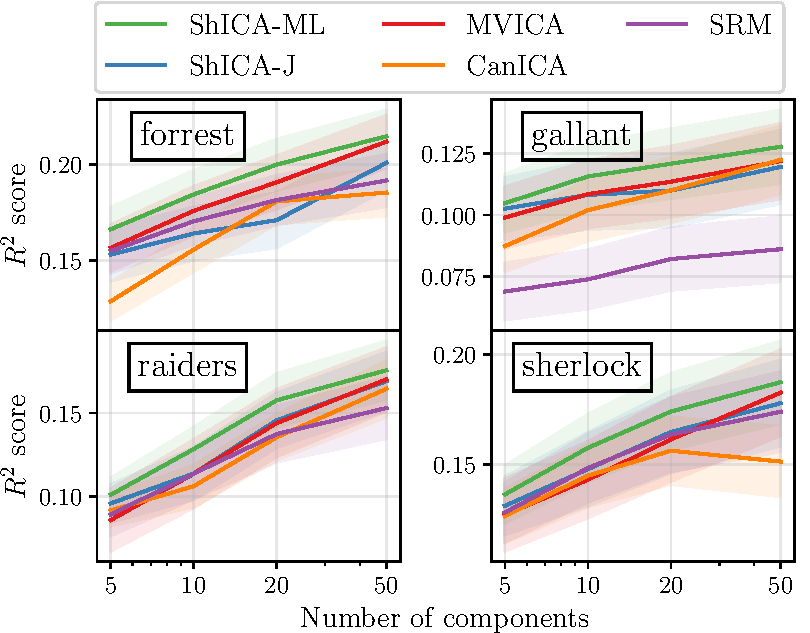
\includegraphics[width=0.99\linewidth]{./figures/amvica/reconstruction.pdf}
  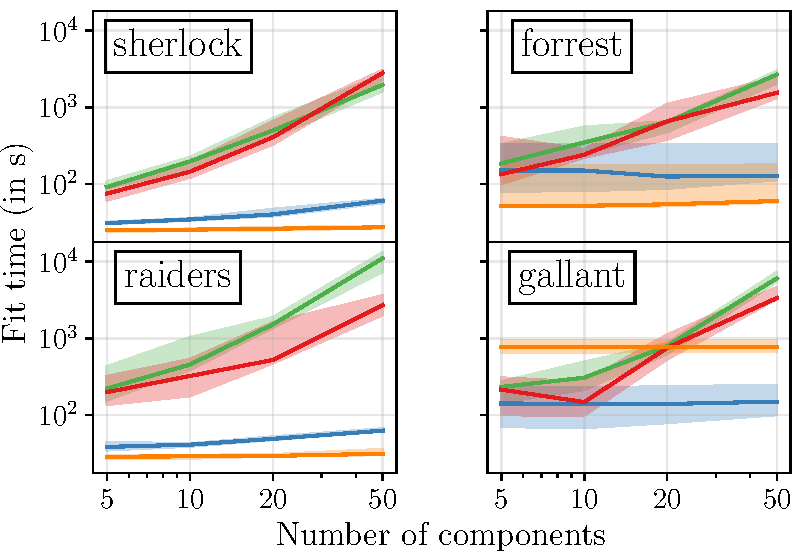
\includegraphics[width=0.99\linewidth]{./figures/amvica/reconstruction_timings.pdf}
  
  \caption{\textbf{Reconstructing the BOLD signal of
      missing subjects}. (\textbf{top}) Mean $R^2$ score between reconstructed data and true
    data. (\textbf{bottom}) Fitting time.
    %\Alex{ylabel should be $R^2$ not R2}
    }
  \label{fig:reconstruction}
\end{wrapfigure}
We reproduce the experimental pipeline of~\cite{richard2020modeling} to benchmark GroupICA methods using their ability to reconstruct fMRI data of a left-out subject.
%
The preprocessing involves a dimension reduction step performed using the shared response model~\cite{chen2015reduced}. Detailed preprocessing pipeline is described in Appendix~\ref{app:preprocessing}. We call an \emph{unmixing operator} the product of the dimension
reduction operator and an unmixing matrix and a \emph{mixing operator} its pseudoinverse. There is one unmixing operator and one mixing operator per view.
The unmixing operators are learned using all subjects
and $80\%$ of the runs. Then they are applied on the remaining $20\%$ of the runs using $80\%$
of the subjects yielding unmixed data from which shared components are extracted. We
then apply the mixing operator of the remaining $20\%$ subjects on the shared components to reconstruct their data.
%
Reconstruction accuracy is measured via the coefficient of determination, \aka
$R^2$ score, that
yields for each voxel the relative discrepancy between the true time course and the predicted one.
% :
% $R^2(\hat{\zb}, \zb) = 1 - \frac{\sum_{t=1}^n (z_t - \hat{z_t})^2}{\sum_{t=1}^n
%   (z_t - \bar{z})^2}$
% where $\bar{z} = \frac1n \sum_{t=1}^n z_t$ is the empirical mean of $\zb$.
%
For each compared algorithm, the experiment is run 25 times with different seeds to obtain error bars. We report the mean $R^2$ score across voxels in a region of interest (see Appendix~\ref{app:preprocessing} for details)
 and display the results in Fig~\ref{fig:reconstruction}. The error bars represent a $95\%$ confidence interval.
The chance level is given by the $R^2$ score of an algorithm that samples the coefficients of its unmixing matrices and dimension reduction operators from a standardized Gaussian. The median chance level is below $10^{-3}$ on all datasets. 
ShICA-ML yields the best $R^2$ score in all datasets and for any number of components. ShICA-J yields competitive results with respect to Multiview ICA while being much faster to fit. A popular benchmark especially in the SRM community is the time-segment matching experiment~\cite{chen2015reduced}: we include such experiments in Appendix~\ref{app:timesegment}.

% AVICA exhibits a small improvement on sherlock and raiders datasets that is
% consistent for different numbers of components (i.e. numbers of components) and competitive results on clips and forrest datasets.

% 

%\pierre{right plot is hard to read, too wide. Lots of space to gain here}

% \section{Conclusion, Future work and Societal impact}
% We introduced the ShICA model as a principled unifying solution to the problems of shared response modelling and GroupICA. ShICA is able to use both the diversity of Gaussian variances and non-Gaussianity for optimal estimation. We presented two algorithms to fit the model: ShICA-J, a fast algorithm that uses noise diversity, and ShICA-ML, a maximum likelihood approach that can separate Gaussian and non-Gaussian components. ShICA algorithms come with principled procedures for shared components estimation, as well as adaptation and estimation of noise levels in each view (subject) and component. On simulated data, ShICA clearly outperforms all competing methods in terms of the trade-off between statistical accuracy and computation time. On brain imaging data, ShICA gives more stable decompositions for comparable computation times, and more accurately predicts the data of one subject from the data of other subjects, making it a good candidate to perform transfer learning. ShICA inherits the ethical questions linked to its field of application. However, as it involves linear transforms, decisions based on its output are easier to interpret. This work can help in brain disease diagnosis and reduce their human and societal burden.

% \section{A fast two-step approach for MIFA}

% While maximum-likelihood approaches possess several important statistical properties that make them attractive, a major drawback is the slowness of the algorithms. 
% %
% These method also require the likelihood to be well defined, and prevents dimension reduction without a more complicated model: for the likelihood to be well defined, we must assume that $A_i$ is square, invertible.
% Instead, we propose a two steps ad-hoc method, based on the following observations that were used for proving identifiability:
% \begin{itemize}
%     \item The knowledge of the empirical covariances $C_{ij}$ for $i\neq j$ allows to recover the mixing matrices $A_i$ up to a global rotation matrix.
%     \item Then, the knowledge of the ``diagonal'' terms $C_{ii}$ allows to eliminate this indeterminacy
% \end{itemize}
% These observations lead to the following two step approach
% \paragraph{Dimension reduction and global estimation}
% We first estimate jointly all the mixing matrices up to a global rotation by minimizing the criterion $\mathcal{L}(A_1, \dots, A_m) = \sum_{i \neq j} \|A_iA_j^{\top} - C_{ij}\|_F^2$.
% Since this cost function is quadratic with respect to each $A_i$, it is easily minimized w.r.t. one of the variable when all others are fixed:

% $$
% \arg\min_{A_i}\mathcal{L}(A_1\dots, A_m) = \left(\sum_{j\neq i} C_{ij}A_j\right)\left(\sum_{j\neq i}(A_j)^{\top}A_j\right)^{-1}
% $$
% Importantly, this formula also holds when the problem is over-determined, i.e. when $A_i\in \mathbb{R}^{p\times d}$ with $d < p$.
% We can then loop over all coordinates several times to obtain a block-coordinate descent algorithm. Each iteration of the algorithm is guaranteed to decrease the loss function. 
% The following lemma shows that minimizing the cost function leads to estimates of the true mixing matrices up to a global indeterminacy.
% \begin{prop}
% Assume that for $i\neq j$, $C_{ij}= B_iB_j^{\top}$ for some matrices $(B_i)_{i=1}^m\in\mathbb{R}^{p\times d}$ with $d< p$. Then, $\mathcal{L}(A_1, \dots, A_m) = 0$ if and only if there exists $U\in\mathcal{O}_d$ such that $A_i = B_i U$ for all $i$.
% \end{prop}
% {\textcolor{red}{Can we say anything about the algorithm ?  does it reach a local / global minimum?}}
% As a consequence, minimizing the previous criterion allows to reduce the dimension of the data. Importantly, since the problem is non-convex, we have no guarantee that the proposed algorithm reaches a global optimum. In practice, we found the proposed method to be robust.
% The last part of the procedure estimates the global rotation $U$ using joint diagonalization.
% \paragraph{Estimation of the global rotation by joint-diagonalization}
% We use the following property to estimation the global rotation.
% \begin{prop} Assume that $C_{ii} = B_i(I_d + D_i)B_i^{\top}$ with $D_i$ a diagonal matrix with positive entries. Let $U$ an  orthogonal matrix, and $A_i = B_i U$, and $K_i = A_i^{-1}C_{ii}A_i^{-\top}$. Then, $U$ is a joint-diagonalizer of the set $K_i$, i.e. the matrices $U^{\top}K_i U$ are all diagonal.
% \end{prop}
% Therefore, letting $A_i$ the outputs of the previous algorithms, we form the matrices $K_i$, and estimate the global rotation $U$ by joint-diagonalization of the $K_i$. The estimate of the mixing matrix is then $A_i U^{\top}$.

%%%%%%%%%%%%%%%%%%%%%%%%%%%%%%%%%%%%%%%%%%%%%%%%%%%%%%%%%%%%
\chapter{Brain decoding and data augmentation}

\chapter{Conclusion}

\bibliographystyle{plain}
\bibliography{biblio}
\
\appendix

\chapter{ShICA}
\section{Proofs and Lemmas}
\subsection{Proof of Theorem~\ref{thm:identif}}
\label{proof:identif}
\begin{proof}
By hypothesis, the covariances verify $C_{ij} =\bbE[\xb_i\xb_j^\top] = A_i(I_p + \delta_{ij}\Sigma_i)A_j^{\top} = A'_i(I_p + \delta_{ij}\Sigma'_i){A'_j}^{\top}$ for all $i, j$. We let $P_i=A_i^{-1}A_i'$. The previous relationship for $j\neq i$ gives $P_iP_j^{\top} = I_p$. Because there are more than 3 views, there is another integer $k \notin\{i,j\}$, and we have $P_iP_k^{\top}= P_jP_k^{\top}=I_p$. This shows that $P_i = P_j$: all these matrices are equal, and we call $P$ their common value. The previous equation also gives $PP^{\top} = I_p$, so $P$ is orthogonal. 
%
We have that $s + n_i$ and $s' + n_i'$ have independent components and $s + n^i = P(s' + n_i')$. Lemma~\ref{lemma:ica} (a direct consequence of classical ICA results~\cite{comon1994independent}, Theorem 10) gives $P=\Pi^{-1} \Omega \Pi'$ where $\Pi$ and $\Pi'$ are sign and permutation matrices such that the first $g$ components of $\Pi(s + n_i)$ and $\Pi'(s' + n_i')$ are Gaussian, and $\Omega$ is a block diagonal matrix given by
\[
\Omega = \begin{bmatrix} \Omega_g & 0 \\ 0 & I_{p - g} \end{bmatrix}
\]
where $\Omega_g$ is orthogonal.
%
We call $A^{(g)}$ the first $g \times g$ block of a matrix $A$ so that $\Omega^{(g)} = \Omega_g$.

Then, considering only the Gaussian components, we can write for $i=j$:  
$(\Pi \Sigma_i)^{(g)} = \Omega_g (\Pi' \Sigma'_i)^{(g)} \Omega_g^{\top}$ for all $i$. This, combined with Assumption~\ref{ass:diversity}, implies that $\Omega_g$ is a sign and permutation matrix (see Lemma~\ref{lemma:eigdecomp}) and therefore $P$ is a sign and permutation matrix. Then it follows that $I + \Sigma_i = P(I + \Sigma'_i)P^{\top}$ and therefore $\Sigma_i = P \Sigma'_i P^{\top}$ so $\Sigma'_i = P^{\top} \Sigma_i P$.
\end{proof}

\subsection{Proof of Theorem~\ref{th:eig}}
\label{proof:eig}
\begin{proof}
  Let us denote $W \in \bbR^{mp \times mp}$ the block diagonal matrix with block $i$ given by
  $(A_i)^{-1}$. We have $C \ub = \lambda D \ub  \iff W C W^\top \zb = \lambda W D W^\top \zb
  $ where $\ub = W^\top \zb$. We call $\zb$ a reduced eigenvector.
  Each
  block in $W C W^\top$ and in $W D W^\top$ is diagonal so any reduced eigenvector $\zb = \begin{bmatrix} \zb_1 \\ \vdots \\ \zb_m \end{bmatrix}$ is
  such that the matrix $Z = [\zb_1 \dots \zb_m]$ has exactly one non-zero line.
  Following Lemma~\ref{lemma:nonzerocoord}, the first $p$ leading reduced
  eigenvectors $\zb^1, \dots, \zb^p$ all have different first non-zero coordinates.
  Therefore the concatenation of the first $p$ leading reduced eigenvectors is given
  by $[\zb^1, \dots \zb^p] = \begin{bmatrix} \Gamma_1 \\ \vdots \\ \Gamma_m \end{bmatrix} P^{\top}$ where $P^{\top} \in \mathbb{R}^{p \times p}$ is a permutation matrix and $\Gamma_i
  \in \mathbb{R}^{p \times p}$ is a diagonal matrix. Therefore, the first $p$
  eigenvectors are given by $[\ub^1 \dots \ub^p] = \begin{bmatrix} W_1^{\top} \\ \vdots \\ W_m^{\top} \end{bmatrix} = \begin{bmatrix} (A_1^{-1})^{\top} \Gamma_1 P^{\top} \\ \vdots \\ (A_m^{-1})^{\top} \Gamma_m P^{\top} \end{bmatrix}$  and so $W_i = P \Gamma_i A_i^{-1}$
\end{proof}


\begin{lemma}
\label{lemma:ica}
Let $\sbb \in \mathbb{R}^k$ and $\sbb'\in \mathbb{R}^k$ have independent components among which $g$ are Gaussian, and $P$ a rotation matrix such that $\sbb = P\sbb'$. Then, $P=\Pi^{-1} O \Pi'$ where $\Pi$ and $\Pi'$ are sign and permutation matrices such that the first $g$ components of $\Pi \sbb$ and $\Pi' \sbb'$ are Gaussian and $O$ is a block diagonal matrix such that $O^{(g)}$, the first $g \times g$ block of $O$, is orthogonal and the other block is identity.
\end{lemma}
\begin{proof}
  From~\cite{comon1994independent}, Theorem 10:
  Assume $\sbb = P\sbb'$, if the column $j$ of $P$ has more than one non-zero element then $s'_j$ is Gaussian. 
  
  Let us define permutations $\Pi_1$, $\Pi'_1$ such that the first $g$ components of $\Pi_1 \sbb$ and $\Pi'_1 \sbb'$ are Gaussian and $P_1  = \Pi_1 P (\Pi'_1)^{-1}$. We can see that $P_1$ is orthogonal.
  
  We have $\Pi_1 \sbb = P_1 \Pi'_1 \sbb'$. So the last $p-g$ columns of $P_1$ contain at most one non-zero element. Using orthogonality of $P_1$ this non-zero element has value $1$ or $-1$ and is also the only one in its line. Let us focus on column $l > g$. Assume column $l$ has its non-zero element at index $k \leq g$. Then line $k$ in $P_1$ is only non-zero at index $l$ and therefore $(\Pi_1 \sbb)_k$ (which is Gaussian) is equal to $(\Pi'_1 \sbb')_l$ (which is not). Therefore column $l$ can only have its non-zero element at an index greater than $g$. This shows that $P_1$ is block diagonal $P_1 = \begin{bmatrix} O_g & 0 \\ 0 & P_2 \end{bmatrix}$ where $O_g$ is orthogonal  and $P_2$ is a sign and permutation matrix.
  \begin{align}
      &\begin{bmatrix} O_g & 0 \\ 0 & P_2 \end{bmatrix} = \Pi_1 P (\Pi'_1)^{-1} \\
      & \iff \begin{bmatrix} O_g & 0 \\ 0 & I \end{bmatrix} \begin{bmatrix} I & 0 \\ 0 & P_2 \end{bmatrix}  = \Pi_1 P (\Pi'_1)^{-1} \\
      & \iff \Pi_1^{-1} \begin{bmatrix} O_g & 0 \\ 0 & I \end{bmatrix} \begin{bmatrix} I & 0 \\ 0 & P_2 \end{bmatrix} \Pi'_1  = P
  \end{align}
  
  Therefore setting $\Pi' =   \begin{bmatrix} I & 0 \\ 0 & P_2 \end{bmatrix} \Pi'_1$ and $\Pi = \Pi_1$ and $O= \begin{bmatrix}O_g & 0 \\ 0 & I  \end{bmatrix}$ concludes the proof.
  
\end{proof}

\begin{lemma}
\label{lemma:eigdecomp}
Assume that Assumption 2 holds for $\Sigma_i$, and that there is an orthogonal matrix $P$ and diagonal matrices $\Sigma_i'$ such that for all $i$, $\Sigma_i' = P\Sigma_iP^{\top}$. Then, $P$ is a permutation matrix.
\end{lemma}
\begin{proof}
The proof is in two parts. First, we show that there exist some coefficients $\alpha_1, \dots, \alpha_m$ such that the matrix $\sum_i\alpha_i\Sigma_i$ has distinct coefficients on the diagonal. Then, since we have $\sum_i\alpha_i\Sigma'_i = P\left(\sum_i\alpha_i\Sigma_i\right)P^{\top}$, and the diagonal $\sum_i\alpha_i\Sigma_i$ has distinct entries, we can invoke the unicity of the eigenvalue decomposition for symmetric matrices, which shows that $P$ is necessarily a permutation matrix.
Now, the only thing left is to prove is that Assumption 2 implies the existence of this linear combination.

We assume by contradiction that any linear combination of the $\Sigma_i$ has two equal entries.

For $\alpha = [\alpha_1, \dots, \alpha_m]$, we let $\mathcal{S}(\alpha) = \diag(\sum_i\alpha_i\Sigma_i)\in\bbR^p$, where $\diag(\cdot)$ extracts the diagonal entries. The operator $\mathcal{S}$ is linear.
%
We now define for $j, j'\leq p$ the linear form $\ell_{jj'}(\alpha) = \mathcal{S}(\alpha)_j - \mathcal{S}(\alpha)_{j'}\in\bbR$. The assumption on the linear combinations of $\Sigma_i$ simply rewrites:
For all $\alpha\in\bbR^m$, there exists $j, j'\leq p$ such that $\ell_{jj'}(\alpha) = 0$.

From a set point of view, this relationship writes
$$
\bigcup_{j, j'}\mathrm{Ker}(\ell_{jj'}) = \bbR^m\enspace.
$$
Since the $\ell_{jj'}$ are all linear forms, the $\mathrm{Ker}(\ell_{jj'})$ are subspaces of dimensions $m$ or $m-1$, and since their union is of dimension $m$, there exists $j, j'$ such that  $\mathrm{Ker}(\ell_{jj'}) = \bbR^m$, i.e. such that $\ell_{jj'} = 0$.

As a consequence, we have for all $\alpha$, $\mathcal{S}(\alpha)_j = \mathcal{S}(\alpha)_{j'}$. This implies that the sequences $(\Sigma_{ij})_i$ and $(\Sigma_{ij'})_i$ are equal, which contradicts Assumption 2.


We have therefore shown that Assumption 2 implies the existence of a linear combination of the $\Sigma_i$ that has distinct entries, which concludes the proof.
\end{proof}


\begin{lemma}
\label{lemma:nonzerocoord}
Let us consider the following eigenvalue problem:
 \begin{align}
  & \begin{bmatrix} I + \Sigma_1 & I & \dots & I \\
    I & I + \Sigma_2 & \ddots & \vdots \\
    \vdots &  \ddots & \ddots & I  \\
    I & \dots & I  &I + \Sigma_m
  \end{bmatrix} \zb = \lambda \begin{bmatrix}
    I + \Sigma_1 & 0 & \dots  & 0 \\
    0 & I + \Sigma_2 & \ddots & \vdots \\
    \vdots & \ddots & \ddots & 0 \\
    0& \dots  & 0 &  I + \Sigma_m  \\
  \end{bmatrix} \zb
  \label{reducedeig}
\end{align}
where $\forall i, \enspace 1 \leq i \leq m, \enspace  \Sigma_m \in \bbR^{p, p}$ are positive diagonal matrices and I is the identity matrix.
If the first $p$ eigenvalues are distincts, the first $p$ eigenvectors $\zb^1, \dots, \zb^p, \zb^i \in \mathbb{R}^{mp}$ have different first non-zero coordinates.
\end{lemma}
%\bt{You implicitly assume that D is the block-diagonal part of C ?}
\begin{proof}
We sort the eigenvectors in $p$ groups of $m$ vectors so that all
vectors in group $l$ have their $l$-th coordinate
different from 0.
Let $\zb^{(l)}$ be an eigenvector in group $l$ and let us call $\wb_l \in
\mathbb{R}^{m}$ the non-zero coordinates of this eigenvector: $\forall i \in \{1 \dots m \}, w_{li} = z^{(l)}_{l + (i-1)p}$.

We have:
\begin{align}
\begin{bmatrix}
  1 + \Sigma_{1l} & 1 & \dots & 1  \\
  1 & 1 + \Sigma_{2l} & \ddots  &\vdots \\
  \vdots & \ddots & \ddots & 1  \\
  1 & \dots & 1 & 1 + \Sigma_{ml}  \\
\end{bmatrix} \wb_l =  \begin{bmatrix}
  1 + \Sigma_{1l} & 0 & \dots  & 0 \\
  0 & 1 + \Sigma_{2l} & \ddots & \vdots \\
  \vdots & \ddots & \ddots & 0 \\
  0& \dots  & 0 &  1 + \Sigma_{ml}  \\
\end{bmatrix} \wb_l \lambda_l
\label{eigsimp}
\end{align}

We now show that the biggest eigenvalue of~\eqref{eigsimp} is strictly above 1 while all
others are strictly below 1. The core of the proof comes from the study of the eigenvalues of a matrix modified by a rank 1 matrix. The reasoning we use here follows~\cite{golub1973some} (end of section 5).

Let us introduce 
$K^l = \diag(\Sigma_{1l} \dots \Sigma_{ml})$ and $\ub = \begin{bmatrix} 1 \\ \vdots \\ 1 \end{bmatrix}$.
Let us drop the index $l$ in the notations for simplicity.

The problem can be rewritten
\begin{align}
  &(\ub \ub^{\top} + K) \wb =  (I + K) \wb \lambda \\
  & \iff (I + K)^{-1}(\ub \ub^{\top} + K) \wb =   \wb \lambda
\end{align}

The characteristic polynomial is given by:
\begin{align}
  &\mathcal{P}(\lambda) = \det( (I + K)^{-1} K - \lambda I + (I + K)^{-1} \ub \ub^{\top}) \label{carpol} \\
  &\propto \det( I + ((I + K)^{-1} K - \lambda I)^{-1}(I + K)^{-1} \ub \ub^{\top})
\end{align}
where we implicitly focus here on eigenvalues $\lambda$ such that $\det((I + K)^{-1} K - \lambda I) \neq 0 \iff \forall i, \lambda \neq \frac{k_i}{1 + k_i}$.

We then use the following property:
Let $A \in \mathbb{R}^{a, b}$ and $B \in \mathbb{R}^{b, a}$ we have
$\det(I_a + AB) = \det(I_b + BA)$.

Let us call $\chi(\lambda) = \det( I + ((I + K)^{-1} K - \lambda I)^{-1}(I + K)^{-1} \ub \ub^{\top})$ we have:
\begin{align}
\chi(\lambda)
  &= 1 + \ub^{\top}((I + K)^{-1} K - \lambda I)^{-1}(I + K)^{-1} \ub \\
  &= 1  + \sum_{i=1}^m \frac1{1 + k_i} \frac1{ \frac{k_i}{1 + k_i} - \lambda}
\end{align}
%\bt{transition from (16) to (17) is not obvious to me !}
where $k_i = \Sigma_{il} > 0$.
% Since $k_i = \Sigma_{il} > 0$, the above secular function is simple to
% study.
% Let us re-order the values $\kappa_i = \frac{k_i}{1 + k_i}$ by increasing
% order $\kappa_1 < \dots < \kappa_m$. The eigenvalues $\lambda_i$ are such that
% $\kappa_1 < \lambda_1 < \kappa_2 < \lambda_2 < \kappa_3 < \dots < \kappa_m <
% \lambda_m$.
% Trivially $\kappa_m < 1$.
Taking the derivative we get 
\begin{align}
\chi'(\lambda) = \sum_{i=1}^m \frac1{1 + k_i} \frac1{ (\frac{k_i}{1 + k_i} - \lambda)^2} > 0
\end{align}

Trivially, $\forall i, \frac{k_i}{1 + k_i} < 1$. We also have
\begin{align}
  \chi(1) = 1 + \sum_{i=1}^{m} \frac1{1 + k_i} \frac1{ \frac{k_i}{1 + k_i} - 1} = 1 - m < 0
\end{align}
 and $\lim_{\lambda \rightarrow + \infty} \chi(\lambda) = 1$ so as $\chi$
 is continuous and strictly increasing on $[1, +\infty[$. Therefore, it reaches $0$ only once on this interval (excluding 1 since we know $\chi(1) \neq 0$). Therefore the greatest eigenvalue $\lambda^*$ is strictly above $1$ while all other eigenvalues are strictly below $1$.
 
  Note that because $\chi' > 0$, $\lambda^*$ is of multiplicity $1$. In the analysis above we ignored those eigenvalues $\lambda$ such that $\lambda = \frac{k_i}{1 + k_i}$ for some $i$. However since $\frac{k_i}{1 + k_i} < 1$, none of these eigenvalues can be the largest one.
 
 Finally, the $p$ first eigenvectors belong to different groups (the
 corresponding eigenvalues are all strictly above 1). This shows that these eigenvectors have
 different first non-zero coordinates. 
 
\end{proof}

% \begin{lemma}
% \label{lemma:rotation}
%   Let us consider the problem $(\Lambda + \delta
%   E)\ub = \ub \psi$ where $\Lambda = \diag(\lambda_1 \dots \lambda_{mp})$ is a diagonal matrix of positive values arranged in decreasing order, $\delta E = o(\lambda_p - \lambda_{p+1})$ and $\delta E = o(\lambda_{pm})$. The first eigenvectors $[\ub^1 \dots  \ub^p]$ are given by
%   $[\ub^1 \dots \ub^p] = [e_1 \dots e_p] \Theta + \delta Z$ where $e_i$ are the vectors of the canonical basis in $\bbR^{mp}$,
%   $\Theta \in \mathbb{R}^{p \times p}$ is a rotation matrix and $\delta Z =
%   O(\delta E)$
% \end{lemma}
% \begin{proof}
%   In matrix form denoting $\Psi = \diag(\psi_1 \dots \psi_{mp})$ the eigenvalues
%   in descending order and $U = [\ub^1 \dots \ub^{mp}]$ the matrix of associated
%   eigenvectors.
%   We want to solve
%   \begin{align}
%     (\Lambda +  \delta E)  U =  U \Psi
%   \end{align}
%   When the difference between any two values of $\Lambda$ is in $O(\min(\lambda_{pm}, \lambda_p - \lambda_{p+1}))$, no
%   rotation indeterminacy appears. We refer the reader to section 3.1 of the tutorial of~\cite{bamieh2020tutorial} to
%   have an explicit formula:
%   $U = I - \Pi \odot \delta E$
%   where $\odot$  is the Hadamar product and
%   $\Pi_{ij} = \begin{cases}
%     0 & \text{if } i =j \\
%     \frac1{\lambda_i - \lambda_j} & \text{if } i \neq i \\
%   \end{cases}$.

%   The rotation indeterminacy appears whenever the difference between two values
%   in $\Lambda$ is of the same order than $\delta E$. In which case we can
%   reparametrize the problem by:
%   \begin{align}
%     (\Lambda' +  \delta E')  U =  U \Psi
%   \end{align}
%   where $\Lambda'$ is obtained by replacing $\lambda_i$ by $\lambda_{i-1}$
%   whenever $\lambda_i - \lambda_{i-1} = O(\delta E)$ and the corresponding terms are
%   added in $\delta E'$ so that we always have $\Lambda + \delta E = \Lambda' +
%   \delta E'$ and $\delta E' = O(\delta E)$.

%   Let us assume without loss of generality that the $l$ first diagonal values of
%   $\Lambda'$ are the same while all others are different. Following derivations in~\cite{bamieh2020tutorial}, the
%   eigenvectors are given by:
%   \begin{align}
%     U = \Theta - \Theta \Pi' \odot \Theta^{\top}\delta E' \Theta
%   \end{align}
%   where $\Theta$ is a matrix such that its first $l, l$ block $\Theta^l$ diagonalizes the
%   first $l, l$ block of $\delta E'$, the off-diagonal blocks are nul and the
%   last diagonal block is identity.
%   \[
%     \Theta = \begin{bmatrix} \Theta^l & 0 \\ 0 & I_{km - l} \\ \end{bmatrix}
%   \]
%   and $\Pi'$ is given by
%   $\Pi'_{ij} = \begin{cases} 0 & \text{if } \lambda_i = \lambda_j \\
%     \frac1{\lambda_i - \lambda_j} & \text{if } \lambda_i \neq \lambda_j
%   \end{cases}$.
  
%   This can be rewritten:
%   \begin{align}
%       [\ub^1 \dots \ub^l] = [\eb_1 \dots \eb_l]\Theta^l
%       [\ub^{l+1} \dots \ub^{pm}] = [\eb_{l+1} \dots \eb_{pm}]
%   \end{align}
%   In particular we see that the eigenvectors are given up to a correction term by the canonical vectors with eigenvalues given (up to a correction term) by the diagonal values in $\Lambda$, but the ones that correspond to the same values of $\lambda_i$ up to $O(\delta_E)$ undergo a rotation $\Theta^l$ that depends on the sampling noise.
  
%   Note that as $\delta E = o(\lambda_p - \lambda_{p+1})$, none of the first $p$ eigenvectors can have the same eigenvalue as the last $pm -p$ up to $O(\delta E)$.
%   Therefore the first $p$ eigenvectors are given by the first $p$ canonical vectors of $\bbR^{pm}$ up to a rotation and a correction term: $[\ub^1 \dots \ub^p] = [e_1 \dots e_p]
%   \mathcal{O} + \delta Z$. Where $\mathcal{O} \in \bbR^{p, p}$ is a rotation and $\delta Z = O(\|\delta E \|_F^2)$.
% \end{proof}
% \bt{I'm lost between $\Theta$ and$ \mathcal{O}$}

\section{Identifiability results for $m< 3$}
\label{app:identifiability}
We have a slightly weaker identifiability result when $m=2$.
\begin{prop}
  \label{prop:identifiability_2d}
  Let $m=2$, and suppose that the scalars $(1 + \Sigma_{1j})(1+\Sigma_{2j})$ for $j=1\dots p$ are all different. We let $\Theta'=(A_1', A_2', \Sigma_1',\Sigma_2')$ that also generates $\xb_1, \xb_2$. Then, there exists a permutation and scale matrix $P$ such that $A'_1 =A_1P$ and $A'_2 = A_2P^{-\top}$.
\end{prop}
\begin{proof}
  We let $P=A_1^{-1}A_1'$. Since $C_{12} = I_p$, it holds 
  $A_2^{-1}A_2'= P^{-\top}$. Then, we have
  $I_p + \Sigma_1 = P(I_p + \Sigma'_1)P^{\top}$. This means that there exists $U\in\mathcal{O}_p$ such that $P = (I_p + \Sigma_1)^{\frac12}U(I_p + \Sigma'_1)^{-\frac12}$. Since $P^{-\top}(I_p+\Sigma'_2)P^{-1} = I_p+\Sigma_2$, we find
  $U(I_p+\Sigma'_1)(I_p+\Sigma'_2)U^{\top} = (I_p+\Sigma_1)(I_p+\Sigma_2)$. By identification, $U$ is a permutation matrix, and $P$ is a scale and permutation matrix.
\end{proof}
As a consequence, when there are only two subjects, it is possible to recover the components and noise levels up to a scaling factor.
%
When there is only one view, $m=1$, there is a global rotation indeterminacy: 
$
A_1(I_p + \Sigma_1)A_1^{\top} = A'_1(I_p + \Sigma_1){A'_1}^{\top}
$
for $A'_1 = A_1(I_p + \Sigma_1)^{\frac12}U(I_p + \Sigma_1)^{-\frac12}$ where $U$ is any orthogonal matrix. In this case, we lose identifiability.

% \section{Derivation of gradient and Hessian for the joint diagonalization}
% \label{app:jointdiag}
% We use a similar approach as\pierre{do we really need the orthogonal algorithm ? anyways, this should be put in appendix} in~\cite{ablin2018beyond} and optimize this loss using a quasi-newton approach. In our case though, we have to take into account the orthogonality constraint.
% In order to take into account orthogonality constraints, the gradient $G$ and Hessian $H$ are defined as 
% $\loss(\exp(\eps) O) = \loss(O) + \langle \eps , G \rangle + \langle \eps , H \eps \rangle + o(\|\eps \|_F^2)$ where $\eps$ is a small skew-symmetric matrix.

% Let us call $D^i = \mathcal{O} \hat{W}_i C_{ii} \hat{W}_i^{\top} \mathcal{O}^{\top}$ and notice that $D^i$ is symmetric.
% We have
% \begin{align}
%     &\loss(\exp(\eps) \mathcal{O}) \\
%     &= \loss((I + \eps + \frac12 \eps^2) \mathcal{O}) + o(\|\eps^2\|) \\
%     &= \frac1{2n} \sum_{i=1}^m \log \det \diag((I + \eps + \frac12 \eps^2) D^i(I + \eps + \frac12 \eps^2)^{\top}) + o(\|\eps^2\|) \\
%     &= \frac1{2n} \sum_{i=1}^m \log \det( \diag(D^i) + \diag(D^i \eps^{\top}) + \diag(\eps D^i) + \\ &\enspace \enspace \enspace \enspace \diag(\eps D^i \eps^{\top}) + \diag(\frac12 \eps^2 D^i) + \diag(\frac12 D^i (\eps^2)^{\top})) + o(\|\eps^2\|)\\
%     &= \frac1{2n} \sum_{i=1}^m \log \det( \diag(D^i) + 2\diag(\eps D^i) + \diag(\eps D^i \eps^{\top}) + 2\diag(\frac12 \eps^2 D^i)) + o(\|\eps^2\|)\\
%     &= \loss(\mathcal{O}) + \frac1{2n} \sum_{i=1}^m \log \det( I + 2\frac{\diag(\eps D^i)}{\diag(D^i)} + \frac{\diag(\eps D^i \eps^{\top})}{\diag(D^i)} + 2\frac{\diag(\frac12 \eps^2 D^i)}{\diag(D^i)}) + o(\|\eps^2\|) \\
%     &= \loss(\mathcal{O}) + \frac1{2n} \sum_{i=1}^m \tr \log( I + 2\frac{\diag(\eps D^i)}{\diag(D^i)} + \frac{\diag(\eps D^i \eps^{\top})}{\diag(D^i)} + 2\frac{\diag(\frac12 \eps^2 D^i)}{\diag(D^i)}) + o(\|\eps^2\|) \\
%     &= \loss(\mathcal{O}) + \frac1{2n} \sum_{i=1}^m \tr( 2\frac{\diag(\eps D^i)}{\diag(D^i)} + \frac{\diag(\eps D^i \eps^{\top})}{\diag(D^i)} \\ &\enspace \enspace \enspace \enspace + 2\frac{\diag(\frac12 \eps^2 D^i)}{\diag(D^i)} - 2(\frac{\diag(\eps D^i)}{\diag(D^i)})^2) + o(\|\eps^2\|) \\
%     &= \loss(\mathcal{O}) + \frac1{2n} \sum_{i=1}^m  \sum_k \left[ \sum_l 2\frac{\eps_{kl} D^i_{lk}}{D^i_{kk}} + \sum_{lm} \frac{\eps_{kl} D^i_{lm} \eps_{km}}{D^i_{kk}} \right.\\  &\left.\enspace \enspace \enspace \enspace + \sum_{lm}\frac{ \eps_{kl} \eps_{lm} D^i_{mk}}{D^i_{kk}} - 2\sum_{lm} \frac{ \eps_{kl}D^i_{lk} \eps_{km}D^i_{mk}}{(D^i_{kk})^2} \right] + o(\|\eps^2\|)
% \end{align}
% By identification we get
% \begin{align}
%     &G_{kl} = \frac1{n} \sum_i \frac{D^i_{lk}}{D^i_{kk}}
%     &H_{klmn} = \frac1{n} \sum_i (\delta_{km} \frac{D^i_{ln}}{D^i_{kk}} + \delta_{lm}\frac{D^i_{nk}}{D^i_{kk}} - 2 \delta_{km} \frac{D^i_{lk} D^i_{nk}}{(D^i_{kk})^2})
% \end{align}

% \begin{align}
%     &G_{kl} = \frac1{n} \sum_i \frac{D^i_{lk}}{D^i_{kk}}
%     &H_{klmn} = \frac1{n} \sum_i (\delta_{km} \frac{D^i_{ln}}{D^i_{kk}} + \delta_{lm}\frac{D^i_{nk}}{D^i_{kk}} - 2 \delta_{km} \frac{D^i_{lk} D^i_{nk}}{(D^i_{kk})^2})
% \end{align}
% We approximate the Hessian by replacing $D^i_{lk}$ by $D^i_{kk} \delta_{lk}$. This approximation is exact when the unmixed covariances are truly diagonal. The approximated Hessian is given by
% $\hat{H}_{klmn} = \frac1{n} \sum_i (\delta_{km} \delta_{ln} \frac{D^i_{ll}}{D^i_{kk}} + \delta_{lm} \delta_{kn} - 2 \delta_{kmln})$.
% Using the fact that $\eps$ is a skew-symmetric matrix

% Let us call $\hat{D^i} = \frac1{n} \sum_i D^i$.
% \begin{align}
% \langle G , \eps \rangle + \frac12 \langle \eps , \hat{H} \eps \rangle &= \sum_{kl} \eps_{kl} G_{kl} + \frac12 \sum_{klmn} \hat{H}_{klmn} \eps_{kl} \eps_{mn} \\
% &= \sum_{kl} G_{kl} \eps_{kl} + \frac12 \left[\sum_{kl} \frac{\hat{D}^i_{ll}}{\hat{D}^i_{kk}} \eps_{kl}^2 + \sum_{kl}\eps_{kl} \eps_{lk} - 2\sum_k \eps_{kk} \right]
% \end{align}
% Using the fact that $\eps$ is anti-symmetric gives:
% \begin{align}
% \langle G , \eps \rangle + \langle \eps , \hat{H} \eps \rangle
% &= \sum_{k} \sum_{l < k} (G_{kl} - G_{lk}) \eps_{kl} + \frac12(\sum_{k} \sum_{l < k} (\frac{\hat{D}^i_{ll}}{\hat{D}^i_{kk}} + \frac{\hat{D}^i_{kk}}{\hat{D}^i_{ll}}) \eps_{kl}^2 -\sum_{k} \sum_{l < k}2\eps_{kl}^2) \\
% &= \sum_{k} \sum_{l < k} (G_{kl} - G_{lk}) \eps_{kl} + \frac12(\sum_{k} \sum_{l < k} \left[\frac{\hat{D}^i_{ll}}{\hat{D}^i_{kk}} + \frac{\hat{D}^i_{kk}}{\hat{D}^i_{ll}} - 2\right] \eps_{kl}^2)
% \end{align}
% So updates are given by
% $\mathcal{O} \leftarrow \exp(J) \mathcal{O}$ where $J_{kl} = \frac{G_{kl} - G_{lk}}{\frac{\hat{D}^i_{ll}}{\hat{D}^i_{kk}} + \frac{\hat{D}^i_{kk}}{\hat{D}^i_{ll}} - 2}$.


\section{Derivation of fixed point updates for scalings}
\label{app:fixedpoint}
\begin{align}
L((\Phi_i)_{i=1}^m)= \sum_i \sum_{j \neq i} \| \Phi_i \diag(Y_{ij}) \Phi_j - I_p \|_F^2
\end{align}
The gradient is given by
\begin{align}
\partialfrac{\Phi_i}{L} = 2\sum_{j \neq i} (\Phi_i \diag(Y_{ij}) \Phi_j - I_p) \Phi_j
\end{align}
Therefore we get
\begin{align}
&\partialfrac{\Phi_i}{L} = 0 \\
&\iff 2\sum_{j \neq i} (\Phi_i \diag(Y_{ij}) \Phi_j - I_p) \Phi_j = 0 \\
&\iff \Phi_i \sum_{j \neq i} \diag(Y_{ij}) \Phi_j^2 - \sum_{j \neq i} \Phi_j = 0 \\
&\iff \Phi_i = \frac{\sum_{j \neq i} \Phi_j}{\sum_{j \neq i} \diag(Y_{ij}) \Phi_j^2}
\end{align}

% \section{Derivation of log-likelihood}
% \label{likelihood_derivation}


% and the log-likelihood writes:
% \begin{align}
%   \mathcal{L} = &\sum_{i=1}^m\left(-\log|W_i| + \frac12 \log |\Sigma_i|\right) + \frac12 \log(|\sum_{i=1}^m \Sigma_i^{-1} + I|) + \frac12 (\sum_{i=1}^m \langle \yb_i , \Sigma_i^{-1} \yb_i \rangle \\&  - \frac12 \langle \left(\sum_{i=1}^m \Sigma_i^{-1} + I \right)^{-1} \sum_{i=1}^m \left(\Sigma_i^{-1} \yb_i \right) , \sum_{i=1}^m \left(\Sigma_i^{-1} \yb_i \right) \rangle)
% \end{align}
% which yields the expected formula.

\section{EM E-step and M-step for ShICA with Gaussian components}
  \paragraph{Notations} We define the usual scalar product for matrices $\langle A , B\rangle = \tr(A^{\top} B)$
  \subsection{E-step}
  \label{conditional_density}
  The complete likelihood is given by
\begin{equation}
  p(\xb, \sbb) = \prod_i p(\xb_i | \sbb) p(\sbb)=  \prod_i (|W_i| \Ncal(\yb_i; \sbb, \Sigma_i)) \Ncal(\sbb; 0, I_k)
\end{equation}

The likelihood writes
\begin{align}
  p(\xbu) &= \int_{\sbb} \prod_{i=1}^m \left(|W_i| \Ncal(\yb_i; \sbb, \Sigma_i) \right) \Ncal(\sbb; 0, I_k) d \sbb \\
\end{align}

Denoting $P = (\sum_{i=1}^m \Sigma_i^{-1} + I)$ we can write
\begin{align}
  &\sum_{i=1}^m \langle \yb_i - \sbb, \Sigma_i^{-1} (\yb_i - \sbb) \rangle + \langle \sbb , \sbb \rangle \\
  &=  \sum_{i=1}^m \langle \yb_i , \Sigma_i^{-1} \yb_i\rangle + \langle \sbb ,(\sum_{i=1}^m \Sigma_i^{-1} + I) \sbb \rangle  -2 \langle \sbb ,\sum_{i=1}^m \left(\Sigma_i^{-1} \yb_i \right) \rangle \\
  &=  \sum_{i=1}^m \left(\langle \yb_i , \Sigma_i^{-1} \yb_i\rangle \right)  +\langle \sbb  - P^{-1}  \sum_{i=1}^m \left(\Sigma_i^{-1} \yb_i \right) , P (\sbb - P^{-1} \sum_{i=1}^m \left(\Sigma_i^{-1} \yb_i \right)) \rangle   \\&- \langle P^{-1} \sum_{i=1}^m \left(\Sigma_i^{-1} \yb_i \right) , \sum_{i=1}^m \left(\Sigma_i^{-1} \yb_i \right) \rangle 
\end{align}
 Therefore we get
 \begin{align}
     p(\sbb | \xb) &= \frac{p(\xb, \sbb)}{p(\xb)} \\
     &= \frac{\exp(-\frac12 \langle \sbb  - P^{-1}  \sum_{i=1}^m \left(\Sigma_i^{-1} \yb_i \right) , P (\sbb - P^{-1} \sum_{i=1}^m \left(\Sigma_i^{-1} \yb_i \right)) \rangle)}{\int_\sbb \exp(-\frac12  \langle \sbb  - P^{-1}  \sum_{i=1}^m \left(\Sigma_i^{-1} \yb_i \right) , P (\sbb - P^{-1} \sum_{i=1}^m \left(\Sigma_i^{-1} \yb_i \right)) \rangle )d \sbb} \\
     &= \mathcal{N}(\sbb; P^{-1} \sum_{i=1}^m \left(\Sigma_i^{-1} \yb_i \right), P^{-1})
 \end{align}
so 
\begin{align}
  &\sbb|\xb \sim \Ncal( \EE[\sbb|\xb], \VV[\sbb | \xb]) \\
  & \text{where } \enspace \EE[\sbb|\xb]= \left(\sum_{i=1}^m \Sigma_i^{-1}  + I \right)^{-1}  \sum_{i=1}^m \left(\Sigma_i^{-1} \yb_i \right) \text{ and } \VV[\sbb|\xb]= (\sum_{i=1}^m \Sigma_i^{-1}  + I)^{-1} \label{MMSE}
\end{align}

\subsection{M-step}
The function to minimize in the M-step is then given by:
\begin{align}
  \Jcal &= -\log p(\xb, \sbb) \\
  &= \sum_{i=1}^m \log(|\Sigma_i|) + \frac12 \tr(\Sigma_i^{-1} \left[(\yb_i - \EE[\sbb | \xb]) (\yb_i - \EE[\sbb | \xb])^{\top}+ \VV[\sbb | \xb]\right]) + c
\end{align}
where $c$ does not depend on $\Sigma_i$

Therefore we get closed-form updates for $\Sigma_i$: 
\begin{align}
\Sigma_i \leftarrow  \diag((\yb_i - \EE[\sbb | \xb]) (\yb_i - \EE[\sbb | \xb])^{\top}+ \VV[\sbb | \xb])
\end{align}
Plugging in the closed-form formula for $\EE[\sbb|\xb]$ and $\VV[\sbb|\xb]$ we get updates that only depends on the covariances $\hat{C_{ij}} = \EE[\xb_i \xb_j^{\top}]$.
\begin{align*}
\Sigma_i \leftarrow \diag(\hat{C_{ii}} - 2 \VV[\sbb | \xb]  \sum_{j=1}^m \Sigma_j^{-1} \hat{C}_{ji}  + \VV[\sbb | \xb]  \sum_{j = 1}^m \sum_{l = 1}^m \left(\Sigma_j^{-1} \hat{C}_{jl} \Sigma_l^{-1} \right) \VV[\sbb | \xb] + \VV[\sbb | \xb])
\end{align*}


\section{EM E-step and M-step for ShICA with non-Gaussian components}
\label{app:emestep}

\paragraph{Notations} We define the usual scalar product for matrices $\langle A , B\rangle = \tr(A^{\top} B)$
  \subsection{E-step}
  The complete likelihood is given by
\begin{align}
  p(\xb, \sbb) &= \prod_i p(\xb_i | \sbb) p(\sbb) \\
  &=  \sum_{\alpha \in \{\frac12, \frac32\}} p(\xb, \sbb | \alpha) 
\end{align}
where 
\[
p(\xb, \sbb | \alpha)  = \prod_i (|W_i| \Ncal(\yb_i; \sbb, \Sigma_i)) \Ncal(\sbb; 0, \alpha I_k)
\]

We denote $P_{\alpha} = (\sum_{i=1}^m \Sigma_i^{-1} + \frac1{\alpha}I), R_{\alpha} =  ((\sum_{i=1}^m \Sigma_i^{-1})^{-1} + \alpha I)$ and $\bar{\yb} = \frac{\sum_i \Sigma_i^{-1} \yb_i}{\sum_i \Sigma_i^{-1}}$. We introduce the constants $c_1, \dots c_3$ that are independent of $\alpha$ and $\sbb$.
We have:
\begin{align}
  p(\xb, \sbb | \alpha) &= \frac{c_1}{|\alpha I|}\exp(-\frac12(\sum_{i=1}^m \langle \yb_i - \sbb, \Sigma_i^{-1} (\yb_i - \sbb) \rangle + \frac1{\alpha}\langle \sbb , \sbb \rangle)) \\
  &= \frac{c_1}{|\alpha I|} \exp(-\frac12(\sum_{i=1}^m \langle \yb_i - \sbb + \bar{\yb} - \bar{\yb}, \Sigma_i^{-1} (\yb_i - \sbb + \bar{\yb} - \bar{\yb}) \rangle + \frac1{\alpha}\langle \sbb , \sbb \rangle)) \\
  &= \frac{c_1}{|\alpha I|} \exp(-\frac12(\sum_{i=1}^m \langle \yb_i - \bar{\yb}, \Sigma_i^{-1} (\yb_i - \bar{\yb}) \rangle + \sum_{i=1}^m \langle \bar{\yb} - \sbb, \Sigma_i^{-1} (\bar{\yb}- \sbb) \rangle + \frac1{\alpha}\langle \sbb , \sbb \rangle)) \\
  &= \frac{c_2}{|\alpha I|} \exp(-\frac12( \langle \bar{\yb} - \sbb, \sum_{i=1}^m  \Sigma_i^{-1} (\bar{\yb}- \sbb) \rangle + \frac1{\alpha}\langle \sbb , \sbb \rangle)) \\
  &= \frac{c_2}{|\alpha I|} \exp(-\frac12( \langle \bar{\yb}, \sum_{i=1}^m  \Sigma_i^{-1} \bar{\yb} \rangle +
  \langle \sbb - P_{\alpha}^{-1} \sum_i \Sigma_i^{-1}\bar{\yb}, P_{\alpha} (\sbb - P_{\alpha}^{-1} \sum_i \Sigma_i^{-1} \bar{\yb}) \rangle \nonumber
   \\& \enspace - \langle P_{\alpha}^{-1} \sum_i \Sigma_i^{-1}\bar{\yb}, \sum_i \Sigma_i^{-1}\bar{\yb} \rangle)) \\
     &= \frac{c_2}{|\alpha I|} \exp(-\frac12( \langle \bar{\yb}, (\sum_{i=1}^m  \Sigma_i^{-1} -  \sum_{i=1}^m  \Sigma_i^{-1} P_{\alpha}^{-1} \sum_{i=1}^m  \Sigma_i^{-1}) \bar{\yb} \rangle + \nonumber \\
  & \enspace \langle \sbb - P_{\alpha}^{-1} \sum_i \Sigma_i^{-1}\bar{\yb}, P_{\alpha} (\sbb - P_{\alpha}^{-1} \sum_i \Sigma_i^{-1} \bar{\yb}) \rangle)) \\
  &= \frac{c_2}{|\alpha I|} \exp(-\frac12( \langle \bar{\yb}, R_{\alpha}^{-1} \bar{\yb} \rangle + \langle \sbb - P_{\alpha}^{-1} \sum_i \Sigma_i^{-1}\bar{\yb}, P_{\alpha} (\sbb - P_{\alpha}^{-1} \sum_i \Sigma_i^{-1} \bar{\yb}) \rangle)) \label{app:51}  \\
  &= c_3 \mathcal{N}(\bar{y}; 0, R_{\alpha}) \mathcal{N}(\sbb, P_{\alpha}^{-1} \sum_i \Sigma_i^{-1}\bar{\yb}, P_{\alpha}^{-1}) \label{app:52}
\end{align}
In equation~\eqref{app:51}, we use the Woodburry matrix identity
$(A + B)^{-1} = A^{-1} - A^{-1} (A^{-1} + B^{-1})^{-1} A^{-1}$ with $A = (\sum_i \Sigma_i^{-1})^{-1}$ and $B = \alpha I$.

In equation~\eqref{app:52}, we use: $|\alpha I | \propto |R_{\alpha}||P_{\alpha}^{-1}|$. Indeed we have:
\begin{align}
&(\sum_{i=1}^m \Sigma_i^{-1} + \frac1{\alpha}I) ((\sum_i \Sigma_i^{-1})^{-1} \alpha I) = \alpha I + (\sum_i \Sigma_i^{-1})^{-1} \\
&\implies P_{\alpha}((\sum_i \Sigma_i^{-1})^{-1} \alpha I) = R_{\alpha} \\
& \implies |P_{\alpha}||\alpha I||(\sum_i \Sigma_i^{-1})^{-1}| = |R_{\alpha}| \\
& \implies |\alpha I | \propto |R_{\alpha}||P_{\alpha}^{-1}|
\end{align}


 Therefore we get
 \begin{align}
     p(\sbb | \xb) &= \frac{\sum_{\alpha} \mathcal{N}(\bar{y}; 0, R_{\alpha}) \mathcal{N}(\sbb, P_{\alpha}^{-1} \sum_i \Sigma_i^{-1}\bar{\yb}, P_{\alpha}^{-1})}{\sum_{\alpha} \mathcal{N}(\bar{y}; 0, R_{\alpha})} \\
 \end{align}
so 

 \begin{align}
  &\sbb|\xb \sim \frac{\sum_{\alpha \in \{\frac12, \frac32 \}}\theta_{\alpha} \Ncal( \eb_{\alpha}, V_{\alpha})}{\sum_{\alpha \in \{\frac12, \frac32 \}}\theta_{\alpha}} \\
  & \text{where } \enspace \eb_{\alpha}= \left(\sum_{i=1}^m \Sigma_i^{-1}  + \frac1{\alpha}I \right)^{-1}  \sum_{i=1}^m \left(\Sigma_i^{-1} \yb_i \right) \text{ and } V_{\alpha} = (\sum_{i=1}^m \Sigma_i^{-1}  + \frac1{\alpha}I)^{-1} \\
  & \text{and } \enspace \theta_{\alpha} = \mathcal{N}((\sum_{i=1}^m \Sigma_i^{-1})^{-1} \Sigma_i^{-1} \yb_i; 0, (\alpha I + \sum_{i=1}^m \Sigma_i^{-1})^{-1})
\end{align}
Therefore we get $\EE[\sbb | \xb] = \frac{\sum_{\alpha \in \{\frac12, \frac32
    \}}\theta_{\alpha} \eb_{\alpha}}{\sum_{\alpha \in
    \{\frac12, \frac32 \}}\theta_{\alpha}}$ and $\VV[\sbb | \xb] = \frac{\sum_{\alpha \in \{\frac12, \frac32
    \}}\theta_{\alpha} \vb_{\alpha}}{\sum_{\alpha \in
    \{\frac12, \frac32 \}}\theta_{\alpha}}$
    

\subsection{M-step}
The function to minimize in the M-step is then given by:
\begin{align}
  \Jcal &= -\log p(\xb, \sbb) \\
  &= \sum_{i=1}^m - \log(|W_i|) + \log(|\Sigma_i|) + \frac12 \tr(\Sigma_i^{-1} \left[(\yb_i - \EE[\sbb | \xb]) (\yb_i - \EE[\sbb | \xb])^{\top}+ \VV[\sbb | \xb]\right]) + c
\end{align}
where $c$ does not depend on $\Sigma_i$ or $W_i$

Therefore we get closed-form updates for $\Sigma_i$: 
\begin{align}
\Sigma_i \leftarrow  \diag((\yb_i - \EE[\sbb | \xb]) (\yb_i - \EE[\sbb | \xb])^{\top}+ \VV[\sbb | \xb])
\end{align}

% and the approximated Hessian $\widehat{\mathcal{H}^{W_i}}$
We update $W_i$ by performing a quasi-Newton step. 
% The gradient $\mathcal{G}^{W_i}$, the Hessian $\mathcal{H}^{W_i}$  are given by
% $\mathcal{G}((I + \epsilon)W_i) = C(W_i) + \langle \epsilon | \mathcal{G}^{W_i} \rangle +
% \frac12 \langle \epsilon | \mathcal{H}^{W_i} \epsilon \rangle$ so
% \begin{align*}
%   &\mathcal{G}^{} = -I + (\Sigma_i)^{-1}(\yb_i - \mathbb{E}[\sbb|\xb])(\yb_i)^{\top} , \enspace \mathcal{H}^{W_i}_{a, b, c, d} = \delta_{a, c} \frac{y_{ib} y_{id}}{\Sigma_i_a}, \enspace \widehat{\mathcal{H}^{W_i}_{a, b, c, d}} =  \delta_{a, c} \delta_{b, d}\frac{(y_{ib})^2}{\Sigma_i_a}
% \end{align*}
% where the Hessian approximation is exact when the unmixed data have truly independent components.

We use the relative gradient $\mathcal{G}^{W_i}$ and $\mathcal{H}^{W_i}$ defined
by \\
$\mathcal{J}(W_i + \varepsilon W_i) = \mathcal{J}(W_i) + \langle
 \varepsilon|\mathcal{G}^{W_i}\rangle + \frac12 \langle
 \varepsilon|\mathcal{H}^{W_i} \varepsilon \rangle$.

 We get:
 \begin{align}
   \mathcal{J}(W_i + \varepsilon W_i) &= \sum_{i=1}^m \left[ -\log(|W_i|) -\log(|I_k + \varepsilon|) - \log(\mathcal{N}(\yb_i + \varepsilon \yb_i; \sbb; \Sigma_i)) \right] + const \\
                                      &= \mathcal{J}(W_i) - \tr(\varepsilon) + \frac12 \tr(\varepsilon^2) \\& \enspace \enspace + \frac12 \left[\langle \varepsilon \yb_i| (\Sigma_i)^{-1} (\yb_i - \sbb) \rangle + \langle (\yb_i - \sbb)| (\Sigma_i)^{-1} \varepsilon \yb_i \rangle + \langle \varepsilon \yb_i| (\Sigma_i)^{-1} \varepsilon \yb_i \rangle \right] \\ & \enspace + o(\|\varepsilon\|^2) \\
   &= \mathcal{J}(W_i) - \sum_a \varepsilon_{a, a} + \frac12 \sum_{a, b} \varepsilon_{a,b} \varepsilon_{b, a} \\& \enspace \enspace + \sum_{a, b} \varepsilon_{a, b} \left[(\Sigma_i)^{-1}(\yb_i - \sbb) (\yb_i)^{\top} \right]_{a, b} + \frac12 \sum_{a, b} \varepsilon_{a, b} \left[(\Sigma_i)^{-1} \varepsilon \yb_i (\yb_i)^{\top}\right]_{a, b} \\ & \enspace + o(\|\varepsilon\|^2) \\
   &= \mathcal{J}(W_i) - \sum_a \varepsilon_{a, a} + \frac12 \sum_{a, b} \varepsilon_{a,b} \varepsilon_{b, a} \\& \enspace \enspace + \sum_{a, b} \varepsilon_{a, b} \left[(\Sigma_i)^{-1}(\yb_i - \sbb) (\yb_i)^{\top} \right]_{a, b} + \frac12 \sum_{a, b, d} \varepsilon_{a, b} (\Sigma_i)^{-1}_{a, a} \varepsilon_{a, d} \left[\yb_i (\yb_i)^{\top}\right]_{d, b} \\ & \enspace + o(\|\varepsilon\|^2) \\
 \end{align}

 So:
 \begin{equation}
 \mathcal{G}^{W_i}_{a, b} =  -\delta_{a,b} + \left[(\Sigma_i)^{-1} (\yb_i - \sbb)(\yb_i)^{\top}\right]_{a, b}
 \end{equation}
 and
 \begin{equation}
 \mathcal{H}^{W_i}_{a, b, c, d} = \delta_{a, d}\delta_{b, c} + \delta_{a, c} \frac{y_{ib} y_{id}}{\Sigma_{ia}}
 \end{equation}
 
 We approximate the Hessian by
 \begin{align}
 \widehat{\mathcal{H}^{W_i}_{a, b, c, d}} = \delta_{ad} \delta_{bc} + \delta_{ac} \delta_{bd}\frac{(y_{ib})^2}{\Sigma_{ia}}
\end{align}
where the Hessian approximation is exact when the unmixed data have truly independent components.

Updates for $W_i$ are then given by
$W_i \leftarrow (I - \rho (\widehat{\mathcal{H}^{W_i}})^{-1} \mathcal{G}^{W_i}) W_i$, 
where $\rho$ is chosen by backtracking line-search.
We alternate between computing the statistics $\mathbb{E}[\sbb|\xb]$ and
$\Var[\sbb|\xb]$ (E-step) and updates of parameters $\Sigma_i$ and $W_i$ for $i=1 \dots m$ (M-step).



\section{fMRI pre-processing pipeline}
\label{app:preprocessing}
All datasets are resampled and  masked using the brain mask available at \url{http://cogspaces.github.io/assets/data/hcp_mask.nii.gz}. Data are detrended and standardized so that they have zero mean and unit variance.  

When reconstructing the BOLD signal of missing subjects, data are preprocessed with a 6~mm smoothing.
In the timesegment matching experiment, we use unsmoothed data except for the sherlock dataset for which the available data are already smoothed.
Multiple acquisitions (called runs) are necessary to build the datasets. Each run lasts approximately 10 minutes.

Sherlock data are available at \url{http://arks.princeton.edu/ark:/88435/dsp01nz8062179}. The precise preprocessing pipeline is described in~\cite{chen2017shared}.
The data are split manually into 4 runs of $395$ timeframes and one run of $396$ timeframes so that cross validation can be performed. Subject 5 is removed because of missing data.

Forrest data are downloaded from OpenfMRI~\cite{poldrack2013toward}. Data are acquired with a 7T scanner with an isotropic spatial resolution of 1~mm and then resampled to a spatial resolution of 3~mm. Details about the acquisition and the task performed are available at ~\url{http://studyforrest.org}. Subject 10 is discarded as not all runs are available at the time of writing. Run 8 is discarded as it is missing in some subjects.

Raiders and Gallant dataset pertains to the Individual Brain Charting dataset. These data were acquired using a 3T scanner and resampled to an isotropic spatial resolution of 3~mm. More information is available in~\cite{ibc}. Gallant dataset is refered to as clips in~\cite{ibc}. Data are available at \url{https://openneuro.org/datasets/ds00268}. Datasets gallant and raiders are preprocessed using FSL \url{http://fsl.fmrib.ox.ac.uk/fsl} using  slice  time  correction,  spatial  realignment,  co-registration  to  the  T1  image  and  affine  transformation  of  the  functional  volumes  to  a  template  brain (MNI). 

A brief summary of the characteristics of the datasets is available in Table~\ref{tab:dataset}
\begin{table}
    \centering
    \begin{tabular}{c|c|c|c|c}
        \textbf{Dataset} & \textbf{Duration} & $m$& \textbf{  Description} \\
        \hline
         Sherlock & 50 min & 16 & Movie watching (BBC TV show "Sherlock") \\
         Forrest & 110 min & 12 & Auditory version "Forrest Gump" \\
         Gallant & 130 min & 12 & various short video clips \\
         Raiders & 110 min & 11 & Movie watching ("Raiders of the lost ark")
    \end{tabular}
    \caption{Information about datasets (name, duration, number of subjects $m$ and short description)}
    \label{tab:dataset}
\end{table}


\section{Additional experiments}
\subsection{Separation performance}
\label{app:separation}
\subsubsection{Separation performance in function of non-Gaussianity}
We generate data according to model~\eqref{eq:model}. Components $\sbb$ are generated using $s_j = d(x)$ with $d(x) = x |x|^{\alpha - 1}$ and $x \sim \mathcal{N}(0, 1)$.   
Mixing matrices $A_i$ are generated by sampling their coefficients from a standardized Gaussian law. The number of samples is fixed to $n=10^5$ and we vary $\alpha$ between $0.8$ and $1.2$. Each experiment is repeated 40 times using different seeds in the random number generator. We use $p=4$ components and $m=5$ views. We display in Fig~\ref{exp:separatingpower} the mean Amari distance across subjects. The experiment is repeated $100$ times using different seeds. We report the median result and error bars  represent the first and last deciles.
 When $\alpha$ is close to 1 (components are almost Gaussian), ShICA-J, ShICA-ML and multiset CCA can separate components well (but multiset CCA reaches higher amari distance than ShICA). In this regime, MultiViewICA yields much higher amari distance than ShICA-J, ShICA-ML or Multiset CCA but is still better than CanICA which cannot separate components at all.
 As non-Gaussianity ($\alpha$) increases, ICA based methods yield better results but ShICA-ML yields uniformly lower amari distance.
\begin{figure}
\centering
  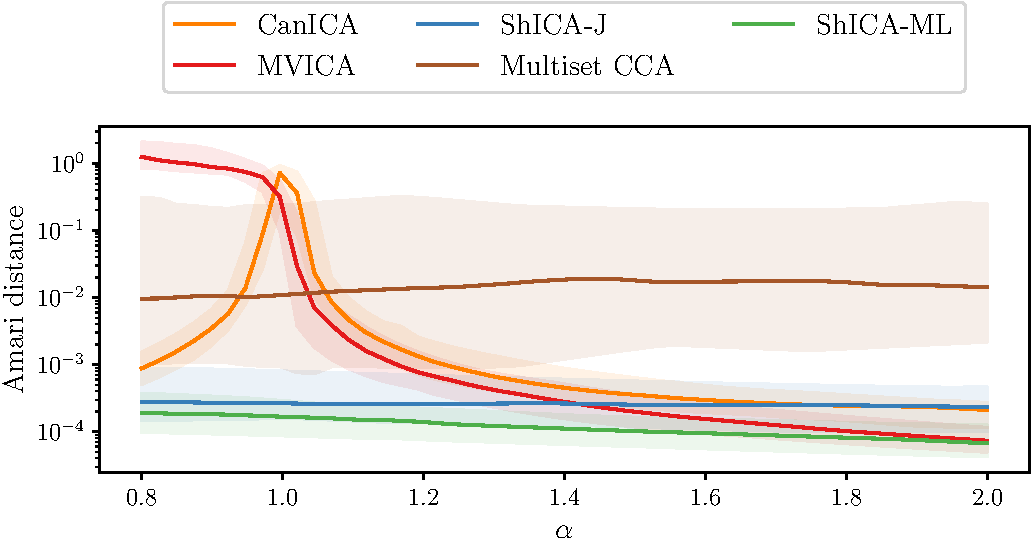
\includegraphics[width=0.8\textwidth]{./figures/amvica/synthetic_gaussian_source.pdf}
  \caption{\textbf{ Separation performance in function of non-Gaussianity} Separation performance of algorithms for sub-Gaussian $\alpha < 1$ and super-Gaussian $\alpha > 1$ components}
  \label{exp:separatingpower}
\end{figure}
\subsubsection{Performance of MultiViewICA on the experiments of Figure~\ref{exp:rotation}}
In the Fig~\ref{exp:rotation2}, we give the performance of MultiViewICA on the same experiment as in Fig~\ref{exp:rotation}.
As we can see, MultiViewICA can separate Gaussian components to some extent and therefore does not completely fail when Gaussian and non-Gaussian components are present. However MVICA is a lot less reliable than ShICA-ML: MVICA is uniformly worse than ShICA-ML and the error bars are very large showing that for some seeds it gives poor results.

\begin{figure}
\centering
  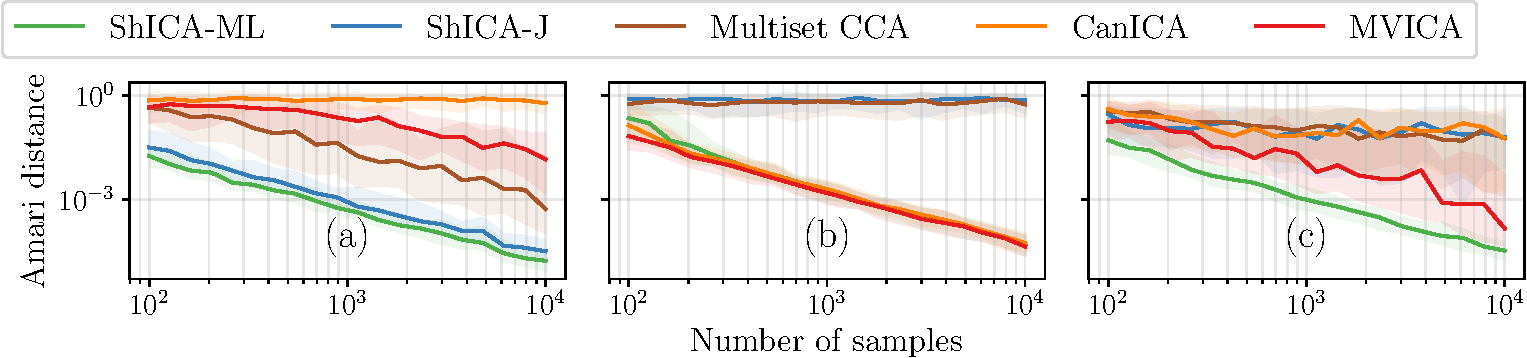
\includegraphics[width=\textwidth]{./figures/amvica/identifiability2.pdf}
  \caption{\textbf{Separation performance}: Algorithms are fit on data following model~\ref{eq:model} \textbf{(a)} Gaussian components with noise diversity \textbf{(b)} Non-Gaussian components without noise diversity \textbf{(c)} Half of the components are Gaussian with noise diversity, the other half is non-Gaussian without noise diversity. }
  \label{exp:rotation2}
\end{figure}

% \begin{figure}
%   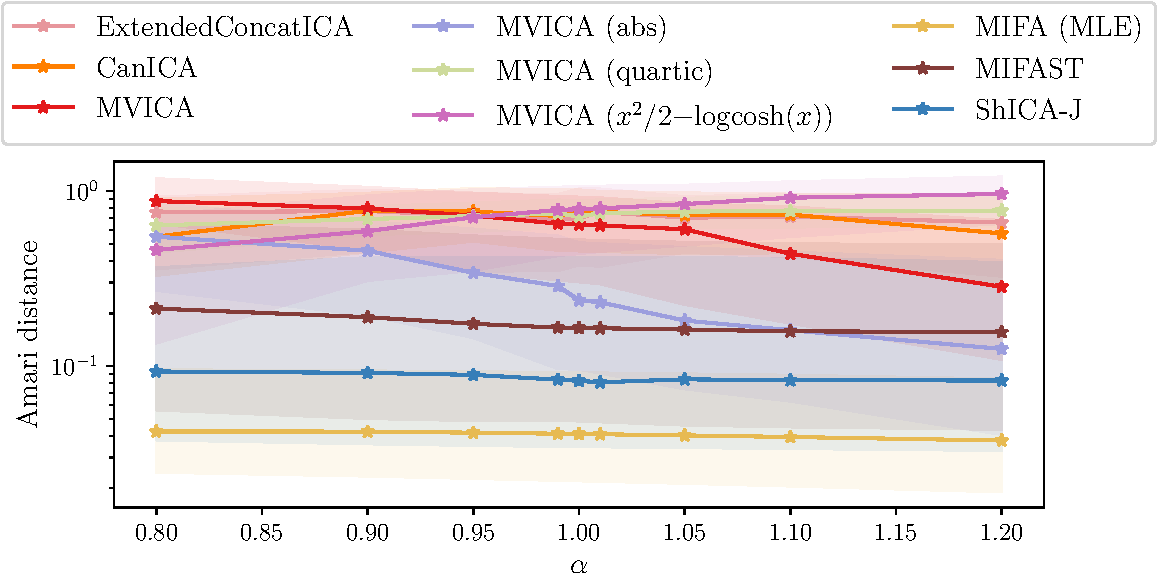
\includegraphics[width=0.5\textwidth]{./figures/synthetic_gaussian_source_50_samples.pdf}
% \end{figure}

\subsection{fMRI timesegment matching experiment}
\label{app:timesegment}
We benchmark ShICA on four different real fMRI datasets via a timesegment matching experiment similar to the one in~\cite{chen2015reduced}. We use full brain data and describe the preprocessing pipeline in Appendix~\ref{app:preprocessing}.
We split the data into a train and test set and algorithms are fitted on the train set.
On the test set, we estimate the shared components from all subjects but one and select a target timesegment containing $9$ consecutive samples in the shared components. We try to localize this timesegment from the components of the left-out subject using a maximum correlation classifier (all possible windows of $9$ consecutive timeframes are considered in the left-out subject excluding the ones partially overlapping with the correct timesegment).
The left panel in Fig~\ref{exp:timesegment} shows that ShICA-ML, MultiViewICA and ShICA-J yield almost equal accuracy and outperform other methods by a large margin. The right panel in Fig~\ref{exp:timesegment} shows that ShICA-J is much faster to fit than MultiViewICA or ShICA-ML.

We would like to highlight here that these experiments are not exactly the same as in~\cite{chen2015reduced} as we use full brain data and they use regions of interest. The code used for this experiment is very similar to the tutorial in \url{https://brainiak.org/tutorials/11-SRM/}. We use the SRM implementation in Brainiak~\cite{kumar2020brainiak}. Also note that the Raiders dataset is different from the one used in~\cite{chen2015reduced} as it involves different subjects and data were acquired in a different neuro-imaging center.

\begin{figure}
    \centering
    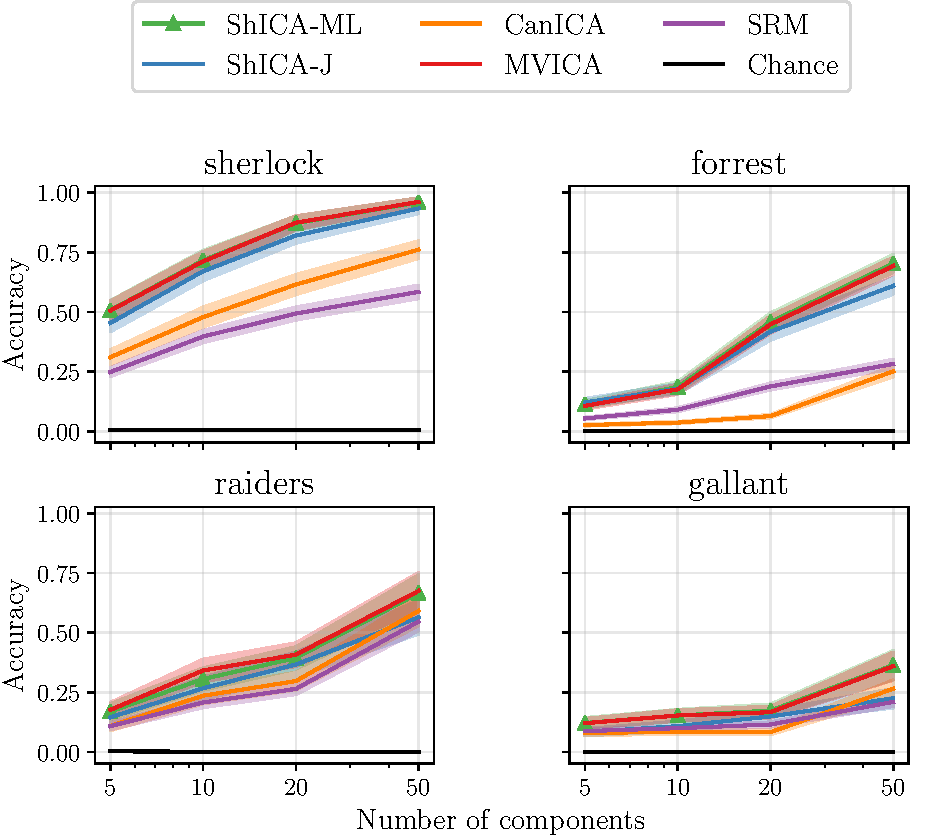
\includegraphics[width=0.45\textwidth]{./figures/amvica/timesegment_matching.pdf}
    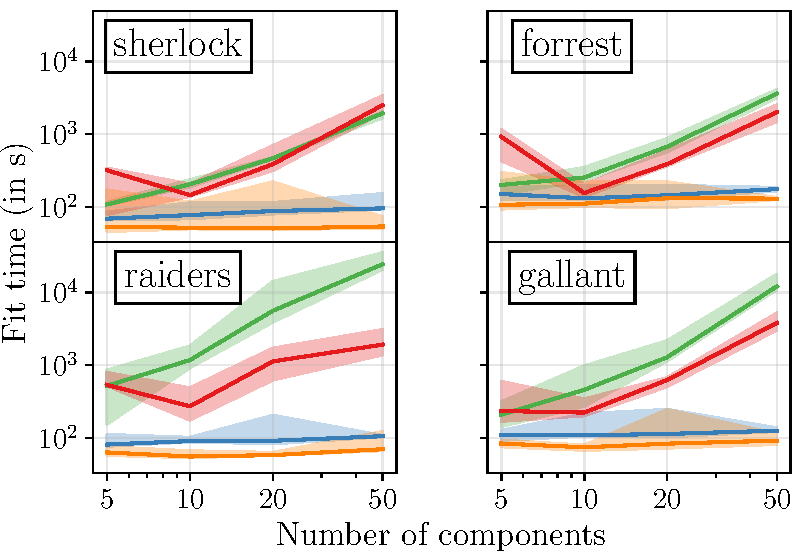
\includegraphics[width=0.45\textwidth]{./figures/amvica/timesegment_matching_timings.pdf}
    \caption{\textbf{Timesegment matching experiment}: (left) Accuracy (right) Fitting time (in seconds)}
    \label{exp:timesegment}
\end{figure}

\subsection{MEG Phantom experiment}
\label{app:phantom}
\subsubsection{Phantom Elektra}
    Dipoles in $m=32$ various locations are emitting the same signal.
    Signal magnitude can be either very high, high or low, leading to 3 datasets: a very clean one, a clean one and a noisy one. These datasets are available as part of the Brainstorm application~\cite{tadel2011brainstorm}. We preprocess the data using Maxwell filtering and low-pass filtering as done in the MNE tutorial \url{https://mne.tools/0.17/auto_tutorials/plot_brainstorm_phantom_elekta.html} and only consider data recorded by the magnetometers.
    We use the very clean dataset to recover the true signal by PCA with 1
    component. Then we reduce the noisy dataset by applying view specific PCA with $k=20$ components and algorithms are applied on the reduced data. We select the component that is closer to the true one and compute the L2 norm between the predicted component and the true one after normalization.
    Then we attempt to recover the position of each dipole by performing dipole fitting on the mixing operator of each view (using only the column corresponding to the true component). The localization error is defined as the mean l2 distance between the true localization and the predicted localization where the mean is computed across dipoles. 
    Each epoch corresponds to 301 samples and 20 epochs are available in total. We vary the number of epochs between 2 and 18 and display in Fig~\ref{exp:meg_phantom} the reconstruction error and the localization error in function of the number of epochs used.
    ShICA-ML outperforms other methods. ShICA-J gives satisfying results while being much faster.
    
    \subsubsection{Phantom Sinusoidal components}
    For completeness, we display the results obtained on another MEG dataset where the true component is a known sinusoidal and $m=8$ different locations are considered for the dipoles. We vary the number of epochs between 2 and 16 and display in Fig~\ref{exp:meg_phantom_neurips} the reconstruction error and the localization error as a function of the number of epochs used. ShICA-ML outperforms other methods. ShICA-J gives satisfying results while being much faster.
    
\begin{figure}
\centering
  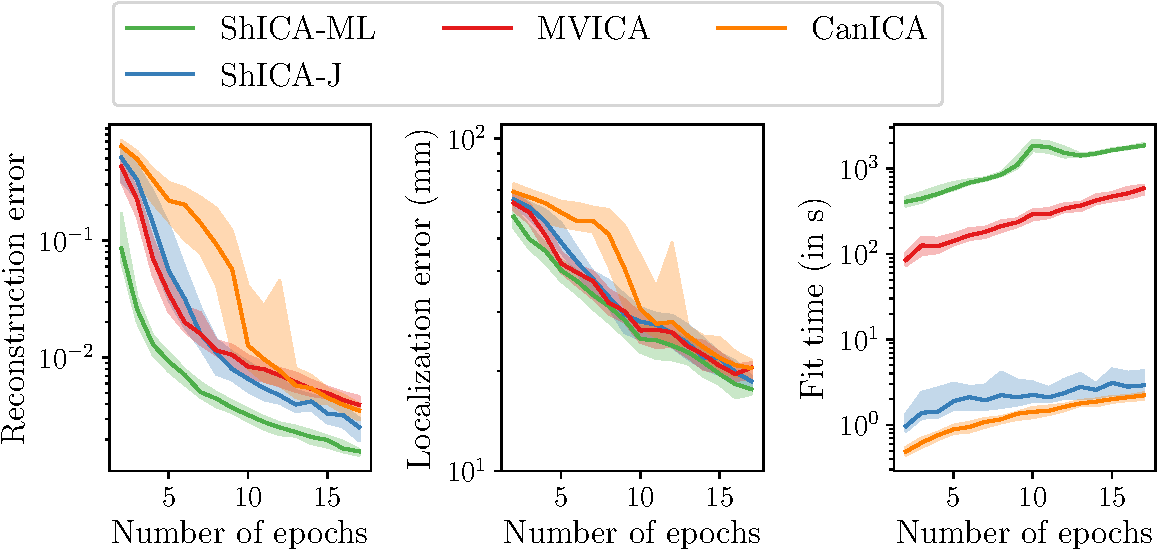
\includegraphics[width=0.7\textwidth]{./figures/amvica/meg_phantom.pdf}
  \caption{\textbf{MEG Phantom (Elektra)}: (left) L2 distance between the predicted and actual component (middle) Mean error (in mm) between predicted and actual dipoles localization (right) Fitting time (in seconds)}
\label{exp:meg_phantom}
\end{figure}

\begin{figure}
\centering
  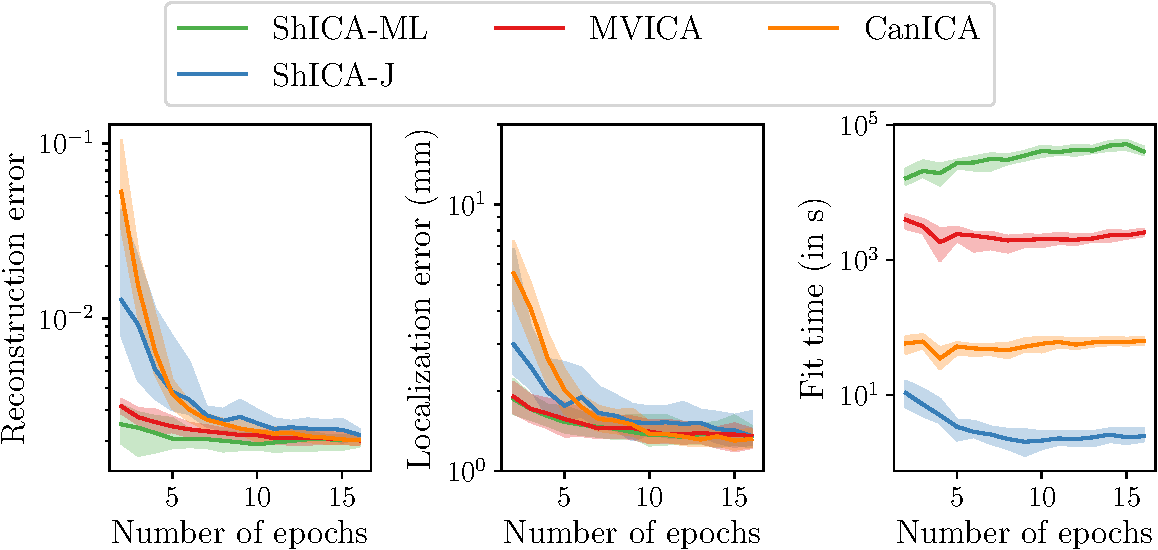
\includegraphics[width=0.7\textwidth]{./figures/amvica/meg_phantom_neurips.pdf}
  \caption{\textbf{MEG Phantom Sinusoidal components}: (left) L2 distance between the predicted and actual component (middle) Mean error (in mm) between predicted and actual dipoles localization (right) Fitting time (in seconds)}
\label{exp:meg_phantom_neurips}
\end{figure}

\subsection{CamCAN MEG components}
We consider the CamCAN dataset used to produce Fig~4. We use $m=496$ subjects and fit ShICA-ML with $p=10$ components. We localize the components of each subject using sLoreta~\cite{pascual2002standardized}. Then components are registered to a common brain and averaged. Thresholded maps are displayed below along with the time courses of each component. Components obtained with ShICA-ML highlight the ventral visual cortex and auditive cortex. The results suggest that the response of the auditive cortex is faster and lasts a shorter time than the response of the ventral visual cortex.

% In contrast, maps obtained with CanICA are very similar and miss the activation in the auditory cortex.
% \subsubsection{Components obtained with ShICA-ML}
{\centering
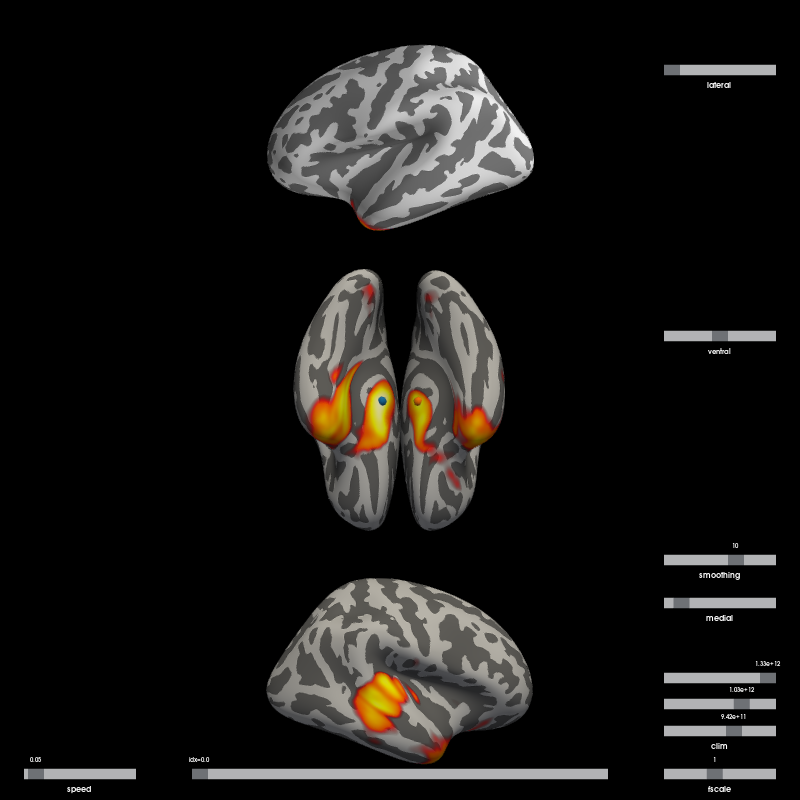
\includegraphics[width=0.4\textwidth]{./figures/amvica/amvica_camcan_montage_0.png}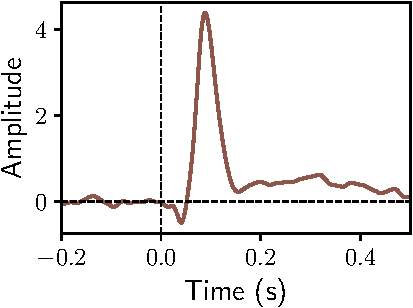
\includegraphics[width=0.4\textwidth]{./figures/amvica/amvica_camcan_source_0.pdf} \\
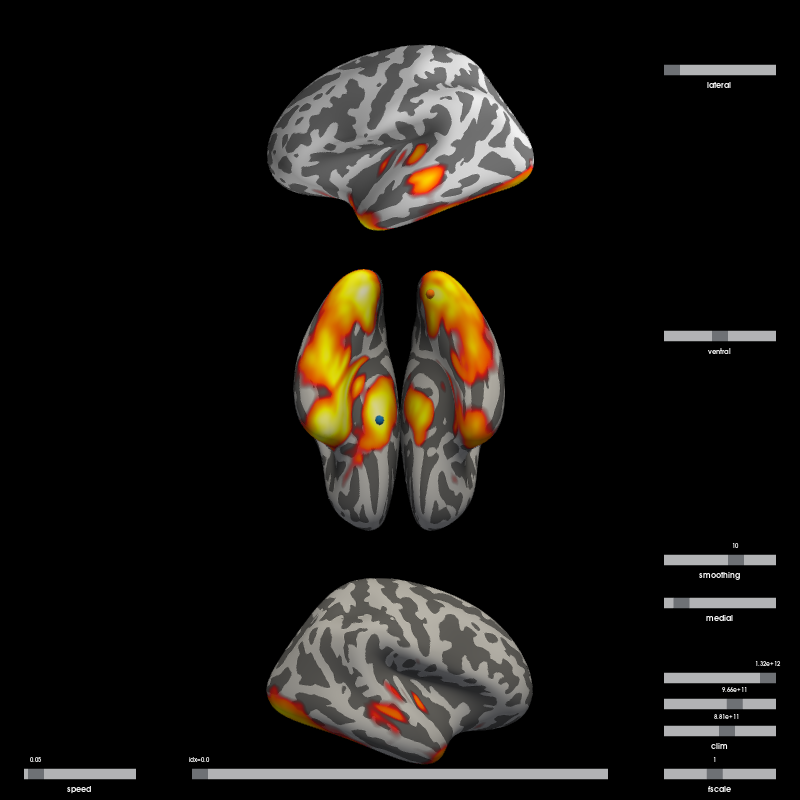
\includegraphics[width=0.4\textwidth]{./figures/amvica/amvica_camcan_montage_1.png}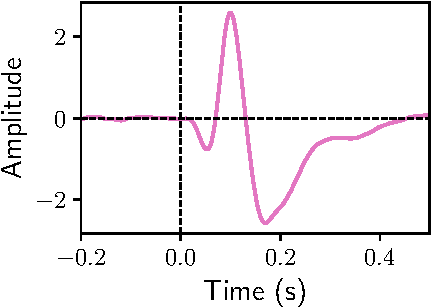
\includegraphics[width=0.4\textwidth]{./figures/amvica/amvica_camcan_source_1.pdf} \\
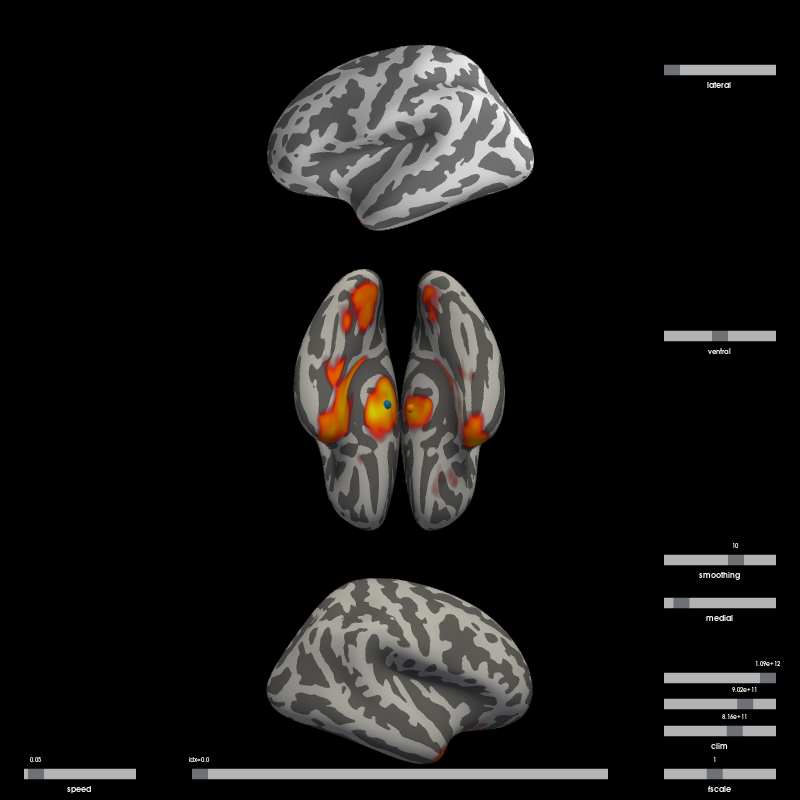
\includegraphics[width=0.4\textwidth]{./figures/amvica/amvica_camcan_montage_2.png}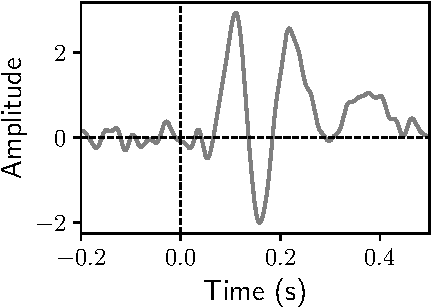
\includegraphics[width=0.4\textwidth]{./figures/amvica/amvica_camcan_source_2.pdf} \\
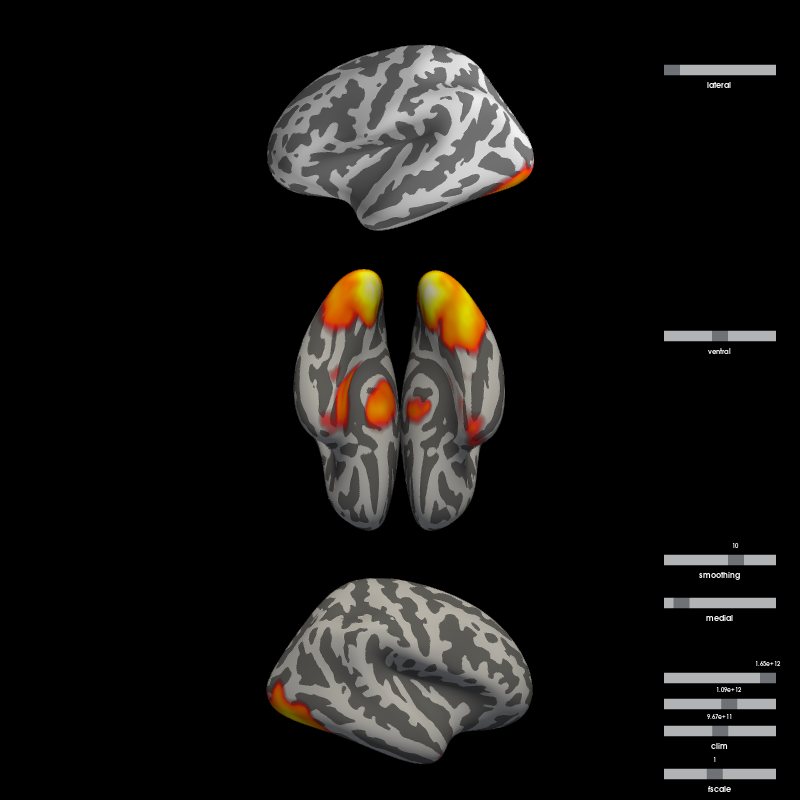
\includegraphics[width=0.4\textwidth]{./figures/amvica/amvica_camcan_montage_3.png}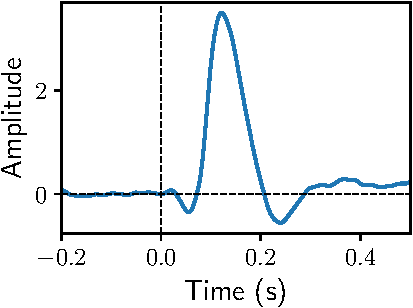
\includegraphics[width=0.4\textwidth]{./figures/amvica/amvica_camcan_source_3.pdf} \\
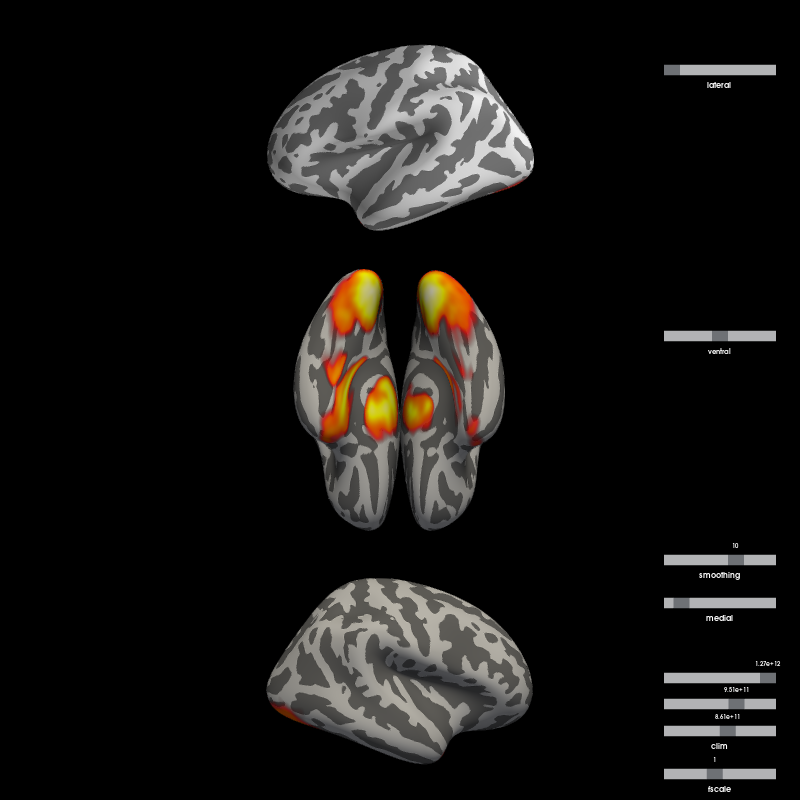
\includegraphics[width=0.4\textwidth]{./figures/amvica/amvica_camcan_montage_4.png}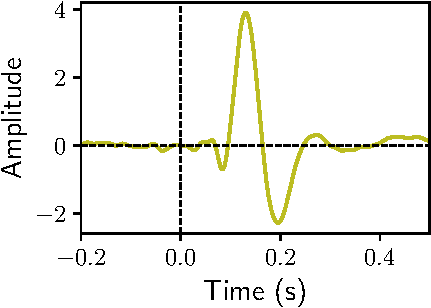
\includegraphics[width=0.4\textwidth]{./figures/amvica/amvica_camcan_source_4.pdf} \\
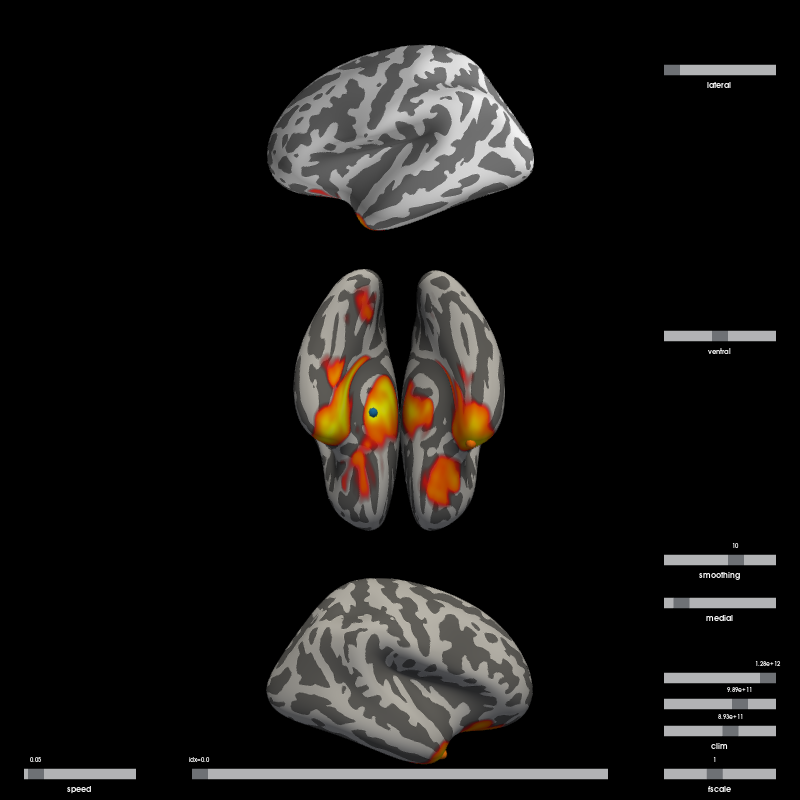
\includegraphics[width=0.4\textwidth]{./figures/amvica/amvica_camcan_montage_5.png}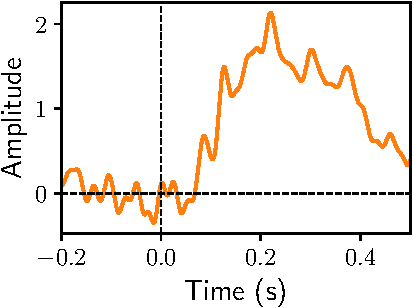
\includegraphics[width=0.4\textwidth]{./figures/amvica/amvica_camcan_source_5.pdf} \\
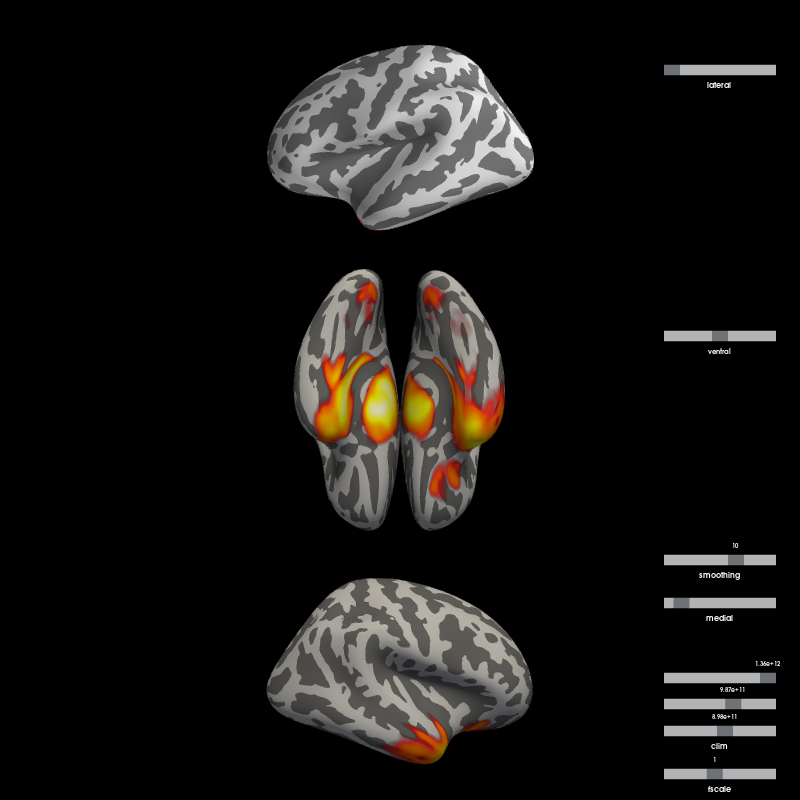
\includegraphics[width=0.4\textwidth]{./figures/amvica/amvica_camcan_montage_6.png}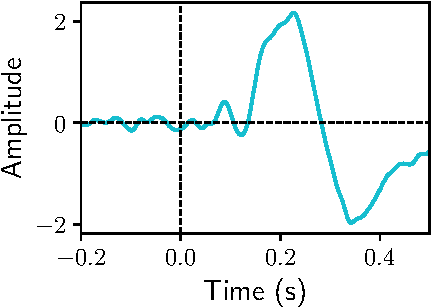
\includegraphics[width=0.4\textwidth]{./figures/amvica/amvica_camcan_source_6.pdf} \\
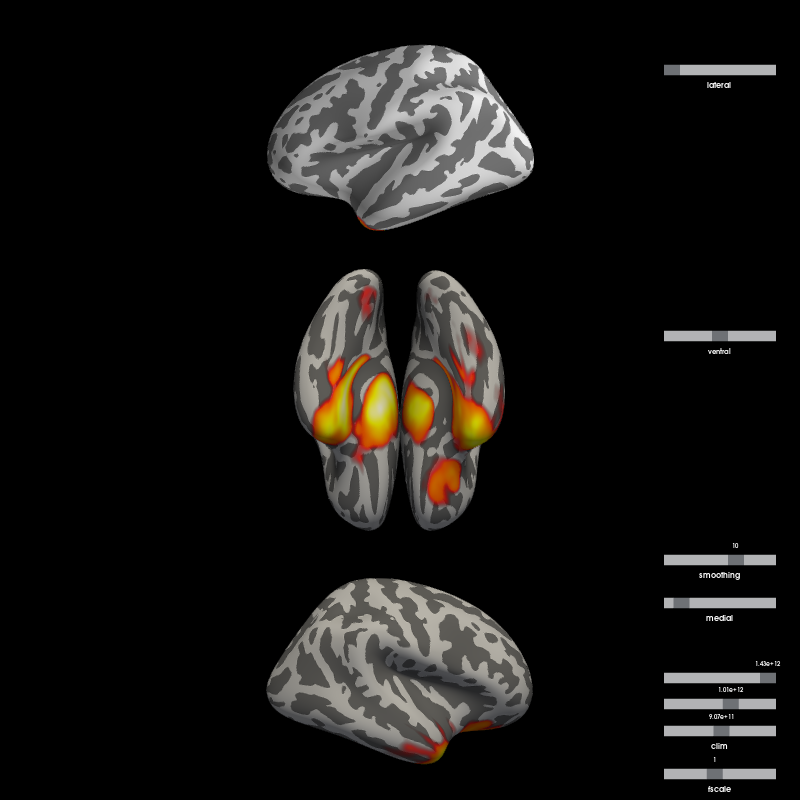
\includegraphics[width=0.4\textwidth]{./figures/amvica/amvica_camcan_montage_7.png}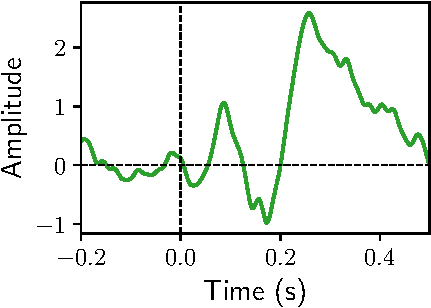
\includegraphics[width=0.4\textwidth]{./figures/amvica/amvica_camcan_source_7.pdf} \\
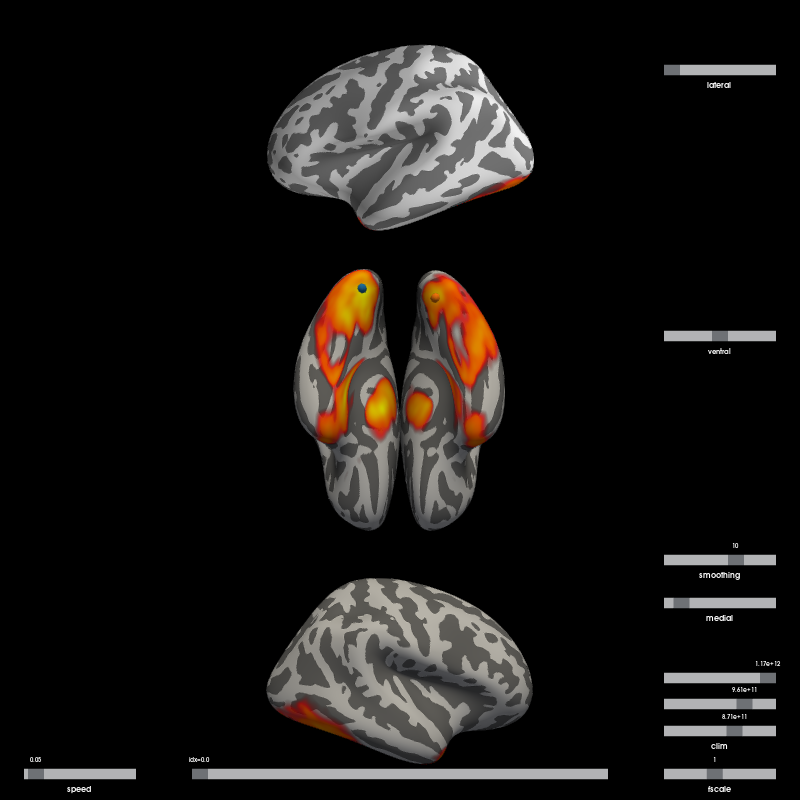
\includegraphics[width=0.4\textwidth]{./figures/amvica/amvica_camcan_montage_8.png}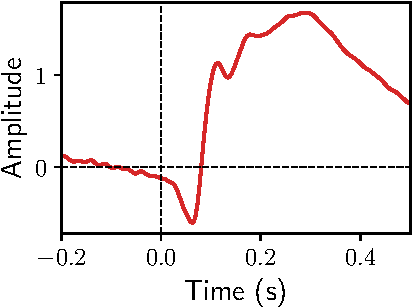
\includegraphics[width=0.4\textwidth]{./figures/amvica/amvica_camcan_source_8.pdf} \\
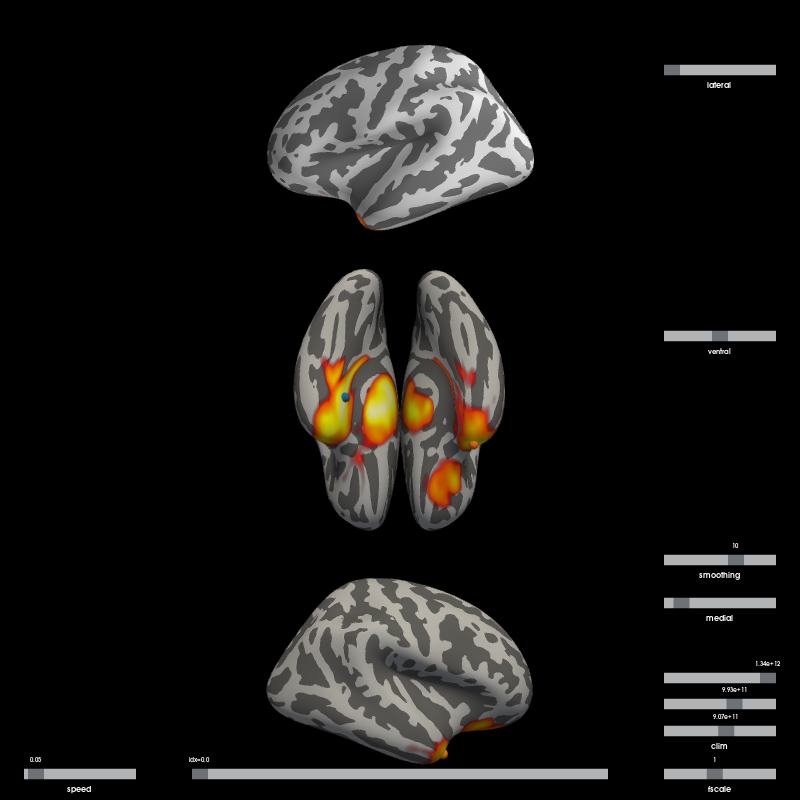
\includegraphics[width=0.4\textwidth]{./figures/amvica/amvica_camcan_montage_9.png}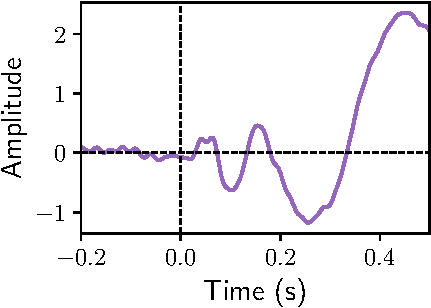
\includegraphics[width=0.4\textwidth]{./figures/amvica/amvica_camcan_source_9.pdf} \\
}
\chapter{MultiViewICA}
\section{Likelihood}
\label{sec:app_likelihood}
\subsection{Initial form of likelihood}\label{sec:appendix:likelihood_transform}

To derive the likelihood, we start by conditioning on $\sbb$. Then, we make a variable transformation from $\xb_i$ to $\nb_i=W_i\xb_i-\sbb$, as opposed to the transformation to $\sbb$ as is usual in ICA. Using the probability transformation formula, we obtain
\begin{equation}
p_{\xb_i|\sbb}(\xb_i|\sbb)=|W_i|p_{\nb_i}(W_i\xb_i-\sbb)    
\end{equation}
where $p_{\nb_i}$ is the density of $\nb_i$. Note that the $\xb_i$ are conditionally independent given $\sbb$, so we have:
\begin{equation}
  p_{\xb|\sbb}(\xb|\sbb)=\prod_{i=1}^m  |W_i| p_{\nb_i}(W_i\xb_i-\sbb)
\end{equation}
and we next get the joint density as:
\begin{equation}
  p_{\xb, \sbb}(\xb,\sbb)=p_{\sbb}(\sbb) \prod_{i=1}^m  |W_i| p_{\nb^i}(W_i\xb_i-\sbb)
\end{equation}
Integrating out $\sbb$ gives Eq.~(\ref{eq:likelihood}).


\subsection{Integrating out the components}\label{sec:appendix:integration}

The integral in question, after factorization, is given by
\begin{equation}
\int_{\sbb} \prod_{j=1}^k \exp \left( -\frac{1}{2\sigma^2} \sum_{i=1}^m ((\wb_j^i)^{\top}\xb_i-s_j)^2 \right) p_{s}(s_j) d\sbb
\end{equation}
which factorizes for each $j$. Denote $y^i_j=(\wb_j^i)^{\top}\xb_i$ and $\tilde{s_j}=\frac1m\sum_{i=1}^m y^i_j$.  Fix $j$, and drop it to simplify notation. Then we need to solve the integral
\begin{align*}
   &\int_s \exp \left(-\frac{1}{2\sigma^2} \sum_{i=1}^m (y^i-s)^2 \right) p_{s}(s)ds\\
   &=\int_s \exp \left(-\frac{1}{2\sigma^2} [ m(\tilde{s}-s)^2 + \sum_{i=1}^m (y^i-\tilde{s})^2] \right) p_{s}(s)ds \\ 
&= \exp \left(-\frac{1}{2\sigma^2}\sum_{i=1}^m (y^i-\tilde{s})^2 \right) 
\int_z \exp \left(-\frac{m}{2\sigma^2} z^2 \right) p_{s}(\tilde{s}-z) dz
\end{align*}

where we have made the change of variable $z=\tilde{s}-s$. The remaining integral simply means that $d$ is smoothed by a Gaussian kernel, which can be computed exactly if $d$ is a Gaussian mixture. We therefore define $f(s) = \log \left(\int_z \exp \left(-\frac{m}{2\sigma^2} z^2 \right) p_{s}(s-z) dz\right)$.
\section{Initialization of MultiViewICA}
\label{sec:app_init}
Since the cost function $\mathcal{L}$ is non-convex, having a good initialization can make a difference in the final result.
% 
We propose a two stage approach.
% 
We begin by applying PermICA on the datasets, which gives us a first set of unimixing matrices $W_1^1, \dots, W_1^m$.
% 
Note that we could also use GroupICA for this task.
% 
Next, we perform a diagonal scaling of the mixing matrices, i.e. we find the diagonal matrices $\Lambda^1, \dots, \Lambda^m$ such that $\mathcal{L}(\Lambda^1W_1^1, \dots, \Lambda^mW_1^m)$ is minimized.
% 
To do so, we employ Algorithm~\ref{algo:mv_ica} but only take into account the diagonal of the descent direction at each step: the update rule becomes $W_i \leftarrow (I_k + \rho \text{Diag}(D))W_i$.
% 
The initial unmixing matrices for Algorithm~\ref{algo:mv_ica} are then taken as $\Lambda^1W_1^1, \dots, \Lambda^mW_1^m$.

Empirically, we find that this two stage procedure allows for the algorithm to start close from a satisfactory solution.
\section{Proofs of Section~\ref{sec:mvica}}
\label{sec:app_proofs}
\subsection{Proof of Prop.~\ref{prop:identifiability}}
\label{app:proof:mvica:identifiability}
We fix a subject $i$. Since $\sbb$ has independent components, so does $\sbb + \nb_i$. Following~\cite{comon1994independent},
Theorem 11, there exists a scale-permutation matrix $P^i$ such that $A'_i =
A_iP^i$. As a consequence, we have $\sbb  + \nb_i = P^i(\sbb' + \nb'^i)$ for all
$i$.

Then, we focus on subject 1 and subject $i \neq 1$:
\begin{align}
  &\sbb + \nb^1 - (\sbb + \nb_i) = P^1(\sbb' + \nb'^1) - P^i(\sbb' + \nb'^i)\\
  &\nb^1 - \nb_i = P^1(\sbb' + \nb'^1) - P^i(\sbb' + \nb'^i)\\
  &\iff P^1\sbb' - P^i\sbb' = P^i \nb'^i - \nb_i + \nb^1 - P^1 \nb'^1 \label{eq:condition_gaussian}
\end{align}
% This shows that $P^1\sbb' - P^i\sbb'$ is Gaussian which can only happen if $P^1= P^i$. 
Since the right hand side of equation (\ref{eq:condition_gaussian}) is a linear combination of Gaussian random variables, this would imply that $P^1\sbb' - P^i\sbb'$ is also Gaussian. However, given that $\sbb'$ is assumed to be non-Gaussian, the equality can only hold if $P^1
= P^i$ and both the right and the left hand side vanish.
Therefore, the matrices $P^i$ are all equal, and there exists a scale and permutation matrix $P$ such that $A'_i = A_iP$.

\subsection{Proof of Prop.~\ref{prop:robust}}
\label{ref:robust}
We consider $W_i = \Lambda (A_i)^{-1}$, where $\Lambda$ is a diagonal matrix.
%
We recall $\xb_i= A_i (\sbb + \nb_i),$ so that $\yb_i = W_i\xb_i= \Lambda(\sbb + \nb_i)$.
%
The gradient of $\loss$ is given by equation~\eqref{eq:gradient}:
\begin{align}
  \mathcal{G}^i &= \frac{1}{m}f'(\tilde{\sbb})(\sbb + \nb_i)^{\top}\Lambda + \frac{1 - 1/m}{\sigma^2} \Lambda\left(\nb_i - \frac{1}{m-1}\sum_{j\neq i} \nb^j\right)(\sbb + \nb_i)^{\top}\Lambda - I_k \\
  & = \frac{1}{m}f'(\Lambda(\sbb + \frac1m\sum_j\nb^j))(\sbb+\nb_i)^{\top} \Lambda + \frac{\sigma'^2(1 - 1/m)}{\sigma^2} \Lambda^2 - I_k
\end{align}
where we write $f'(\sbb) = \begin{bmatrix}f'(s_1) \\ \vdots \\ f'(s_k) \end{bmatrix}$.
Therefore, $\mathcal{G}^i$ is diagonal and constant across subjects (because $f'(\Lambda(\sbb + \frac1m\sum_j\nb^j))(\nb_i)^{\top} = f'(\Lambda(\sbb + \frac1m\sum_j\nb^j))(\nb^{i'})^{\top}$).
Let us therefore consider only its coefficient $(a, a)$, and let $\lambda = \Lambda_{aa}$:
$$
\mathcal{G}^i_{aa} =G(\lambda) = \phi(\lambda)\lambda + \frac{\sigma'^2(1 - 1/m)}{\sigma^2}\lambda^2 - 1,
$$
where $\phi(\lambda) = \frac{1}{m}f'(\lambda(s_a + \frac1m\sum_j n^j_a))(s_a+n_a^i)$. One the one hand, we have $G(0) = -1$. On the other hand, if we assume for instance that $f'$ has sub linear growth (i.e. $|f'(x)| \leq c|x|^{\alpha} +d$ for some $\alpha < 1$) or that $\phi$ is positive, we find that $G(+\infty) = +\infty$.
Therefore, $G$ cancels, which concludes the proof.

\subsection{Stability conditions}
\label{sec:stability}
We consider $W_i = \Lambda (A_i)^{-1}$ where $\Lambda$ is such that the gradients $\mathcal{G}^i$ all cancel. We consider a small relative perturbation of $W_i $ of the form $W_i \leftarrow (I_k + E^i)W_i$, and consider the effect on the gradient.
We define $\Delta^i=\mathcal{G}^i\left((I_k + E^1)W_1, \dots, (I_k + E^m)W_m\right)$.
Denoting $C = \frac{1 - 1/ m}{\sigma^2}$ and $\tilde{\nb} = \frac1m\sum_{i=1}^m \nb_i$, we find:
\begin{align}
     &\Delta^i=\underbrace{\frac1m f'\left(\Lambda(\sbb + \tilde{\nb}) + \frac1m \sum_{j=1}^m E^j\Lambda(\sbb +\nb^j)\right)(\sbb +\nb_i)^{\top}\Lambda(I_k + E^i)^{\top} }_{\Delta_1^i} +\\
     &C\underbrace{\left(\Lambda\nb_i - \frac{1}{m-1}\sum_{j\neq i} \Lambda\nbb^j + E^i\Lambda(\sbb + \nb_i) - \frac{1}{m-1}\sum_{j\neq i} E^j \Lambda(\sbb + \nb^j)\right)(\sbb + \nb_i)^{\top}\Lambda(I_k + E^i)^{\top}}_{\Delta_2^i} \\
     &- I_k\\
\end{align}

The first term is expanded at the first order, denoting $S = \sum_{j=1}^m E^j$:

\begin{align}
    \Delta_1^i &= \frac1m \left(f'(\Lambda(\sbb + \tilde{\nb})) + f''(\Lambda(\sbb + \tilde{\nb}))\odot \left(\frac1m \sum_{j=1}^m E^j\Lambda(\sbb +\nb^j)\right)\right)(\sbb +\nb_i)^{\top}\Lambda(I_k + E^i)^{\top}\\
    &=\frac1m f'(\Lambda(\sbb + \tilde{\nb}))(\sbb + \nb_i)^{\top}\Lambda(I_k + E^i)^{\top} + \frac1{m^2}S\odot  \left(f''(\Lambda(\sbb + \tilde{\nb}))(\sbb^2)^{\top}\Lambda^2 \right)\\
    &+\frac{1}{m^2}E^i\odot\left(f''(\Lambda(\sbb + \tilde{\nb}))((\nb_i)^2)^{\top}\Lambda^2 \right)
\end{align}
The symbol $\odot$ denotes the element-wise multiplication, $f'(\sbb) = \begin{bmatrix}f'(s_1) \\ \vdots \\ f'(s_k) \end{bmatrix}$ and $f''(\sbb) = \begin{bmatrix}f''(s_1) \\ \vdots \\ f''(s_k) \end{bmatrix}$.
Similarly, the second term gives at the first order: 
\begin{align}
    \Delta_2^i &= \sigma'^2\Lambda^2(I_k + E^i)^{\top} + (1 + \sigma'^2)E^i\Lambda^2 - \frac{1}{m-1} (S - E^i) \Lambda^2
\end{align}

Combining this, we find:

\begin{align}
 \Delta^i = (E^i)^{\top} + E^i \odot\Gamma^E
 +S\odot \Gamma^S
\end{align}
where 
$$
\Gamma^E= \left(\frac1{m^2}f''(\Lambda(\sbb + \tilde{\nb}))((\nb_i)^2)^{\top} + (1-\frac1m)\frac{\sigma'^2}{\sigma^2} + \frac{1}{\sigma^2} \right)\Lambda^2
$$
$$
\Gamma^S =\left(\frac1{m^2}f''(\Lambda(\sbb + \tilde{\nb}))(\sbb^2)^{\top} -\frac{1}{m\sigma^2}  \right)\Lambda^2
$$

are $k\times k$ matrices, independent of the subject.
This linear operator is the Hessian block corresponding to the $i$-th subject:
Denoting $\mathcal{H}$ the Hessian, it is the mapping $\mathcal{H}(E^1, \dots, E^m) = (\Delta^1, \dots, \Delta^m)$.

The coefficient $\Delta^i_{ab}$ only depends on $(E^i_{ab}, E^i_{ba}, E^1_{ab},\dots, E^m_{ab})$. Therefore, the Hessian is block diagonal with respect to the blocks of coordinates $(E^1_{ab}, E^1_{ba}, \dots, E^m_{ab}, E^m_{ba})$. Denote $\varepsilon = \Gamma^E_{ab}$, $\varepsilon' = \Gamma^E_{ba}$, $\beta = \Gamma^S_{ab}$ and $\beta'= \Gamma^S_{ba}$. The linear operator for the block is:

$$
K(\varepsilon, \varepsilon', \beta, \beta')=
\left(
    \begin{array}{ll|ll|l|ll}
\varepsilon + \beta & 1       & \beta & 0       & \dots  & \beta & 0       \\
1      & \varepsilon' + \beta' & 0      & \beta' & \dots  & 0      & \beta' \\
\hline
\beta & 0       & \varepsilon + \beta & 1       &        & \beta & 0       \\
0      & \beta' & 1      & \varepsilon' + \beta' & \ddots & 0      & \beta' \\
\hline
\vdots & \vdots  &        & \ddots  & \ddots & \vdots & \vdots  \\
\hline
\beta & 0       & \beta & 0       & \dots  & \varepsilon + \beta & 1       \\
0      & \beta' & 0      & \beta' & \dots  & 1      & \varepsilon' + \beta'
    \end{array}
\right)
$$
The positivity of $\mathcal{H}$ is equivalent to the positivity of this operator for all pairs $a, b$.
We now assume $\beta \beta' > 0$.

First, we should note that $K(\varepsilon, \varepsilon', \beta, \beta') $ is congruent to $K(\varepsilon \sqrt{\frac{\beta'}{\beta}}, \varepsilon' \sqrt{\frac{\beta}{\beta'}}, \sqrt{\beta\beta'}, \sqrt{\beta\beta'})$ via the basis $\text{diag}((\frac{\beta'}{\beta})^{1/4}, (\frac{\beta}{\beta'})^{1/4}, \cdots,(\frac{\beta'}{\beta})^{1/4}, (\frac{\beta}{\beta'})^{1/4})$.
%
We denote to simplify notation $\alpha = \varepsilon \sqrt{\frac{\beta'}{\beta}}$, $\alpha' = \varepsilon' \sqrt{\frac{\beta}{\beta'}}$ and $\gamma = \sqrt{\beta\beta'}$. We only have to study the positivity of $K(\alpha, \alpha', \gamma, \gamma)$.
We have:
$$
K(\alpha, \alpha', \gamma, \gamma) =  I_m  \otimes M_\alpha+ \gamma  \mathbb{1}\otimes I_2, \enspace M_\alpha = 
\begin{pmatrix}
\alpha & 1 \\
1 & \alpha'
\end{pmatrix}
$$
Since $I_m\otimes M_\alpha$ and $\gamma \mathbb{1}\otimes I_2$ commute, the minimum value of $\text{Sp}(K)$ is $\text{min}(I_m\otimes M_\alpha) + \text{min}(\gamma\text{Sp}(\mathbb{1}))=\frac12(\alpha + \alpha' - \sqrt{(\alpha - \alpha')^2 + 4}) + m\min(0, \gamma)$.
Since we assumed $\beta \beta' > 0$ we have $\gamma > 0$. This is similar to the usual ICA case, we find that the condition is $\alpha\alpha' > 1$.

If the following conditions hold for all pair of components $a, b$, the components are a local minimum of the cost function:
\begin{itemize}
    \item $\Gamma^S_{ab}\Gamma^S_{ba}\geq 0$
    \item $\Gamma^E_{ab}\Gamma^E_{ba} > 1$
\end{itemize}
\section{Identifiability for Shared Response Model}
\label{sec:app_identifiability}
The shared response model~\cite{chen2015reduced} (SRM) models the data $\xb_i \in \bbR^v$ of subject $i$ for $i = 1,\dots, m$ as
\begin{align*}
    \xb_i = A_i \sbb + \nb_i \enspace \text{with} \enspace \sbb \sim \Ncal(0, \Sigma), \enspace\nb_i \sim \Ncal(0, \rho_i^2 I_v), \enspace {A_i}^{\top}A_i = I_k
\end{align*}
where $A_i \in \bbR^{v, k}$, $\sbb \in \bbR^p$ and  $\Sigma \in \mathbb{R}^{k, k}$ is a symmetric positive definite matrix.

\begin{proposition}
SRM is not identifiable
\end{proposition}
\begin{proof}
Let us assume the data $\xb_i \enspace i=1, \dots, m$ follow the SRM model with parameters $\Sigma, A_i, \rho_i^2 \enspace i=1, \dots, m$. 

Let us consider an orthogonal matrix $O \in \Ocal_k$.
We call $A'_i = A_i O$ and $\Sigma' = O^{\top} \Sigma O$. 
$\Sigma'$ is trivially symmetric positive definite.

Then the data also follows the SRM model with different parameters $\Sigma', A'_i, \rho_i^2 \enspace i=1, \dots, m$.
\end{proof}

\begin{proposition}
We consider the decorrelated SRM model with an additional decorrelation assumption on the shared responses.
\begin{align*}
\xb_i = A_i \sbb + \nb_i \enspace \text{with} \enspace \sbb \sim \Ncal(0, \Sigma), \enspace\nb_i \sim \Ncal(0, \rho_i^2 I_v), \enspace {A_i}^{\top}A_i = I_k
\end{align*}
where $\Sigma$ is a positive \emph{diagonal} matrix. We further assume that the values in $\Sigma$ are all distinct and ranked in ascending order.
The decorrelated SRM is identifiable up to sign indeterminacies on the columns of 
$\begin{bmatrix}
A_1 \\
\vdots \\
A_m
\end{bmatrix}
$.
\end{proposition}
\begin{proof}
The decorrelated SRM model can be written
\begin{align*}
    &\xb_i \sim \Ncal(0, A_i \Sigma {A_i}^{\top} + \rho_i^2 I_v) \enspace \text{with}\enspace  {A_i}^{\top}A_i = I_k
\end{align*}
where $\Sigma$ is a positive diagonal matrix with distincts values ranked in ascending order.

Let us assume the data $\xb_i \enspace i=1, \dots, m$ follow the decorrelated SRM model with parameters $\Sigma, A_i, {\rho_i}^2 \enspace i=1, \dots, m$. Let us further assume that the data $\xb_i \enspace i=1, \dots, m$ follow the decorrelated SRM model with an other set of parameters $\Sigma', A'_i, {\rho'_i}^2 \enspace i=1, \dots, m$.

Since the model is Gaussian, we look at the covariances.
We have for $i \neq j$
\begin{align*}
    \bbE[\xb_i\left(\xb_j\right)^{\top}] = A_i\Sigma {A^j}^{\top} = A'_i \Sigma'{A'^j}^{\top} \enspace, 
\end{align*}
The singular value decomposition is unique up to sign flips and permutation. Since eigenvalues are positive and ranked the only indeterminacies left are on the eigenvectors. For each eigenvalue a sign flip can occur simultaneously on the corresponding left and right eigenvector.

Therefore we have $\Sigma' = \Sigma$, $A_i = A'_i D^{ij}$ and $A^j = A'^j D^{ij}$ where $D^{ij} \in \bbR^{k, k}$ is a diagonal matrix with values in $\{-1, 1\}$. This analysis holds for every $j \neq i$ and therefore $D^{ij} = D$ is the same for all subjects.

We also have for all $i$
\begin{align*}
    \bbE[\xb_i \left(\xb_i\right)^{\top}] = A_i \Sigma {A_i}^{\top} + \rho_i^2 I_v =  A'_i \Sigma' {A'_i}^{\top}  + {\rho'}_i^2 I_v\\
\end{align*}
We therefore conclude ${\rho'}_i^2 = \rho_i^2, i=1 \dots m$.

Note that if the diagonal subject specific noise covariance $\rho_i^2 I_v$ is replaced by any positive definite matrix, the model still enjoys identifiability.
\end{proof}

\section{fMRI experiments}
\label{sec:app_expts}
\subsection{Dataset description and preprocessing}
\label{preprocessing}
The full brain mask used to select brain regions is available in the Python package associated with the paper.

\paragraph{Sherlock}
In \emph{sherlock} dataset, 17 participants are watching "Sherlock" BBC TV show (beginning of episode 1). 
%
These data are downloaded from \url{http://arks.princeton.edu/ark:/88435/dsp01nz8062179}. 
%
Data were acquired using a 3T scanner with an isotropic spatial resolution of 3 mm. 
%
More information including the preprocessing pipeline is available in~\cite{chen2017shared}.
%
Subject 5 is removed because of missing data leaving us with 16 participants.
%
Although \emph{sherlock} data are downloaded as a temporal concatenation of two runs, we split it manually into 4 runs of 395 timeframes and one run of 396 timeframes so that we can perform 5 fold cross-validation in our experiments.


\paragraph{FORREST}
In FORREST dataset 20 participants are listening to an audio version of the Forrest Gump  movie.
%
FORREST data are downloaded from OpenfMRI~\cite{poldrack2013toward}. 
%
Data were acquired using a 7T scanner with an isotropic spatial resolution of 1~mm (see more details in~\cite{hanke2014high}) and resampled to an isotropic spatial resolution of 3~mm.
%
More information about the forrest project can be found at \url{http://studyforrest.org}.
%
Subject 10 is discarded because not all runs available for other subjects were available for subject 10 at the time of writing.
%
Run 8 is discarded because it is not present in most subjects.
 
\paragraph{RAIDERS}
In RAIDERS dataset, 11 participants are watching the movie "Raiders of the lost ark".
% 
The RAIDERS dataset belongs to the Individual Brain Charting dataset~\cite{ibc}.
% 
Data were acquired using a 3T scanner and resampled to an isotropic spatial resolution of 3~mm.
% 
The RAIDERS dataset reproduces the protocol described in~\cite{haxby2011common}.
%
Preprocessing details are described in~\cite{ibc}.

\paragraph{CLIPS}
In CLIPS dataset, 12 participants are exposed to short video clips. 
%
The CLIPS dataset also belongs to the Individual Brain Charting dataset (\cite{ibc}).
%
Data were acquired using a 3T scanner and resampled to an isotropic spatial resolution of 3~mm.
%
It reproduces the protocol of original studies described in \cite{nishimoto2011reconstructing} and \cite{huth2012continuous}.
%
Preprocessing details are described in~\cite{ibc}.

At the time of writing, the CLIPS and RAIDERS dataset from the individual brain charting dataset \url{https://project.inria.fr/IBC/} are available at \url{https://openneuro.org/datasets/ds002685}.
%
Protocols on the visual stimuli presented are available in a dedicated repository on Github: \url{https://github.com/hbp-brain-charting/public_protocols}.
% The informed consent of all subjects was obtained before scanning.
% Bertrand: There is no reason you deal with that

\subsection{Reconstructing the BOLD signal of missing subjects: Discussion on ROIs choice}
\label{brainmaps}

The quality of the reconstructed BOLD signal varies depending on the choice of the region of interest. In Figure~\ref{fig:brainmaps}, we plot for GroupICA, SRM and MultiViewICA, the R2 score per voxel using 50 components for datasets \emph{sherlock}, \emph{forrest}, \emph{raiders} and \emph{clips}. As could be anticipated from the task definition, \emph{forrest} obtains high reconstruction accuracy in the auditory cortices, while \emph{clips} shows good reconstruction in the visual cortex (occipital lobe mostly); the richer \emph{sherlock} and \emph{raiders} datasets yield good reconstructions in both domains, but also in other systems (language, motor).
%
We also see visually see that data reconstructed by MultiViewICA are
a better approximation of the original data than other methods.
%
This is particularly obvious for the \emph{clips} datasets where it is
clear that voxels in the posterior part of the superior
temporal sulcus are better recovered by MultiViewICA than by SRM or
GroupICA.

In order to determine the ROIs, we focus on the R2 score per voxel between the BOLD signal reconstructed by GroupICA and the actual bold signal. We run GroupICA with $10, 20$ and $50$ components and select the voxels that obtained a positive R2 score for all sets of components.
%
We discard voxels with an R2 score above 80\% as they visually correspond to artefacts and apply a binary opening using a unit cube as the structuring element. The chosen regions are plotted in figure~\ref{fig:roi}.

\begin{figure}
  \centering
  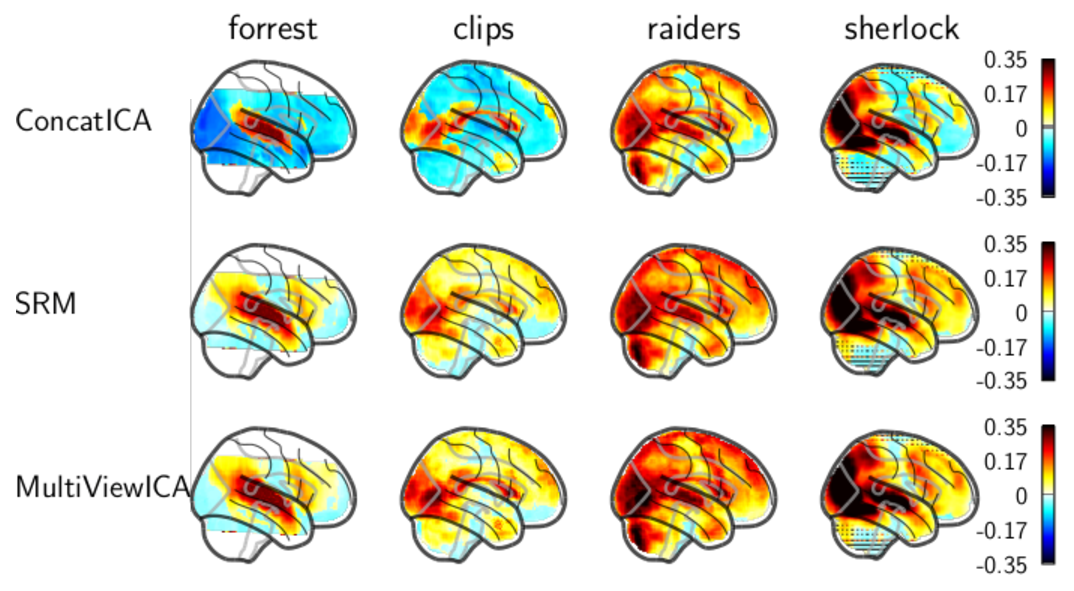
\includegraphics[width=\textwidth]{figures/mvica/reconstruction_score_fullbrain.pdf}
  \caption{\textbf{Reconstructing the BOLD signal of missing subjects: Reconstruction R2 score per voxel} We plot for GroupICA, SRM and MultiViewICA, the R2 score per voxel using 50 components for datasets \emph{sherlock}, \emph{forrest}, \emph{raiders} and \emph{clips}. We visually see that data reconstructed by MultiViewICA are more faithful reproduction of the original data than other methods.}
  \label{fig:brainmaps}
\end{figure}

\begin{figure}
  \centering
  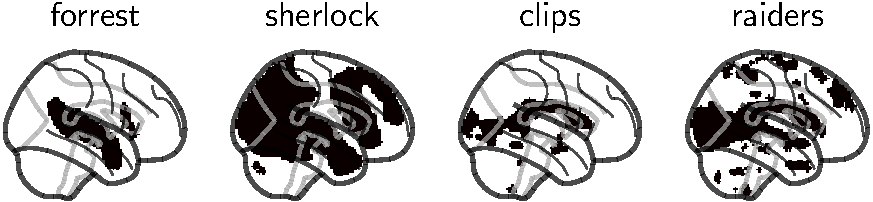
\includegraphics[width=\textwidth]{figures/mvica/reconstruction_score_roi.pdf}
  \caption{\textbf{Data-driven choice of ROI} Chosen ROIs for the experiment: Reconstructing the BOLD signal of missing subjects.}
  \label{fig:roi}
\end{figure}

\subsection{Between-runs time-segment matching}
\label{app_spatialmaps}

\begin{figure}
  \centering
  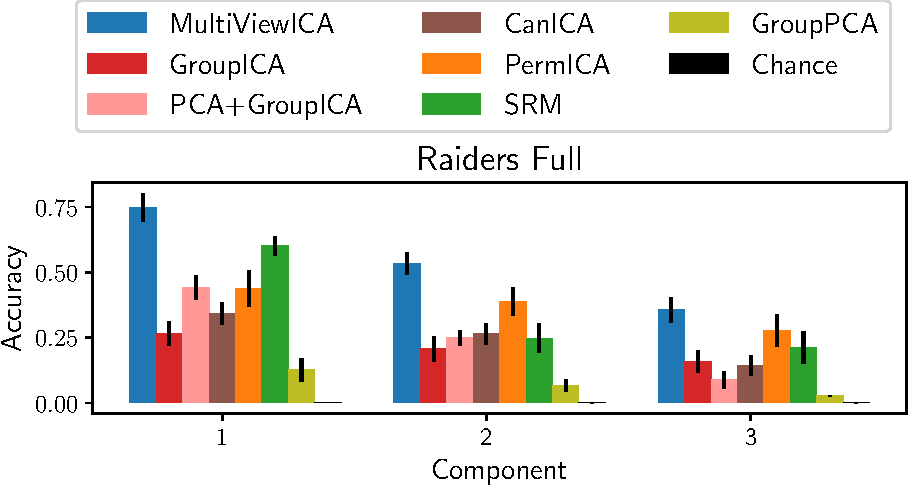
\includegraphics[width=\textwidth]{figures/mvica/swetha_exp_full_fit.pdf}
  \caption{\textbf{Between runs time-segment matching}. Interesting components correlates more when they correspond to the same stimulus (same scenes of the movie) than when they correspond to distinct stimuli (different scenes).
  %We show that when MultiView ICA is used, we can locate a target time-segment in one session using the data of another session corresponding to the same stimuli.
  We extract 20 components and report the mean accuracy of the 3 best performing components}
  \label{fig:swetha}
\end{figure}

We measure the ability of each algorithm to extract meaningful shared components that correlate more when they correspond to the same stimulus than when they correspond to distinct stimuli. We use the \emph{raiders-full} dataset, which allows this kind of analysis because subjects watch some selected scenes from the movie twice, during the first two runs (1 and 2) and the last two (11 and 12).
%
First, the forward operators are learned by fitting each algorithm with 20 components on the data of all 11 subjects using all 12 runs. We then select a subset of 8 subjects and the shared components are computed by applying the forward operators and averaging.
%
We select a large target time-segment ($50$
timeframes) taken at random from run 1 and 2, and we try to localize the corresponding sample time-segment from the 10 last runs using a single component of the shared components.
%
The time-segment is said to be
correctly classified if the correlation between the target and corresponding sample
time-segment is higher than with any other time-segment (partially overlapping windows are excluded).
%
In contrast to the \emph{between subject time-segment matching} experiment, we obtain one accuracy score per component.
%
We repeat the experiment 10 times with different subsets of subjects randomly chosen and report the mean accuracy of the 3 best performing components in Figure~\ref{fig:swetha}. Error bars correspond to a 95~\% confidence interval.
%
MultiView ICA achieves the highest accuracy.

We then focus on the 3 best performing components of MultiView ICA. For each component, we plot in Figure~\ref{fig:app_spatialmaps} (left) the shared components during two sets of runs where subjects were exposed to the same scenes of the movie. We then study the localisation of these components.
%
We average the forward operators across subjects and plot the columns corresponding to the components of interest in Figure~\ref{fig:app_spatialmaps} (right).
%
As each column is seen as a set of weights over all voxels, it represents a spatial map.

The component 1 of the shared responses follows almost the same pattern in the two set of runs corresponding to the same scenes of the movie. The spatial map corresponding to component 1 highlights the language network.
%
In component 2, the temporal patterns during the viewing of identical scenes are also very similar. The corresponding spatial map highlights the visual network especially the visual dorsal pathway.
%
In component 3, there exists a similarity however less striking than with the two previous components. The corresponding spatial map highlights a contrast between the spatial attention network and the auditory network.

\begin{figure}
  \centering
  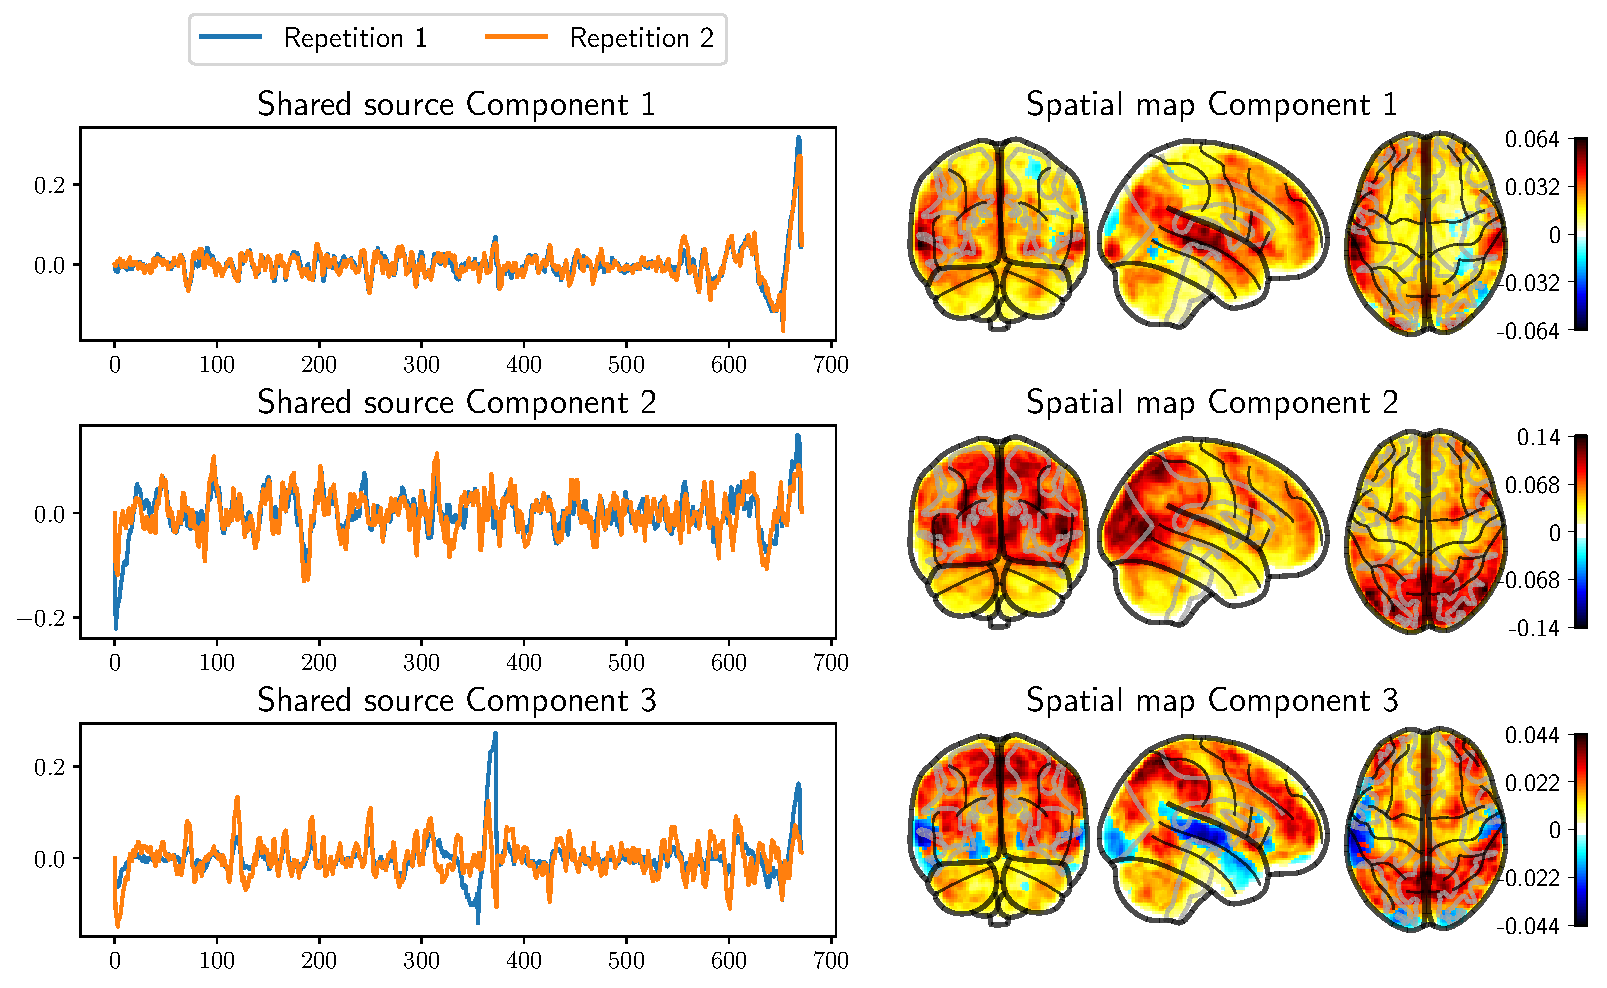
\includegraphics[width=\textwidth]{figures/mvica/swetha_exp_full_fit_appendix.pdf}
  \caption{\textbf{Between-runs time segment matching: spatial maps and timecourses} \emph{Left:} Timecourses of the 3 shared components yielding the highest accuracy. The two displayed set of runs correspond to the same scenes in the movie. \emph{Right:} Localisation of the same shared components in the brain}
  \label{fig:app_spatialmaps}
\end{figure}

\subsection{Reproducing time-segment matching experiment}
\label{appendix_reproduce}
We reproduce the time-segment matching experiments described in \cite{chen2016convolutional} and \cite{zhang2016searchlight} and use two fold classification over runs instead of 5-fold as we have done in the main paper. We used the sherlock data available at \url{http://arks.princeton.edu/ark:/88435/dsp01nz8062179} and the full brain mask provided in the Python package associated with the paper. We applied high-pass filtering (140 s cutoff) and the time series of each voxel were normalized to zero mean and unit variance.

The results are available in Figure~\ref{fig:supp_timesegment}.

\begin{figure}
  \centering
  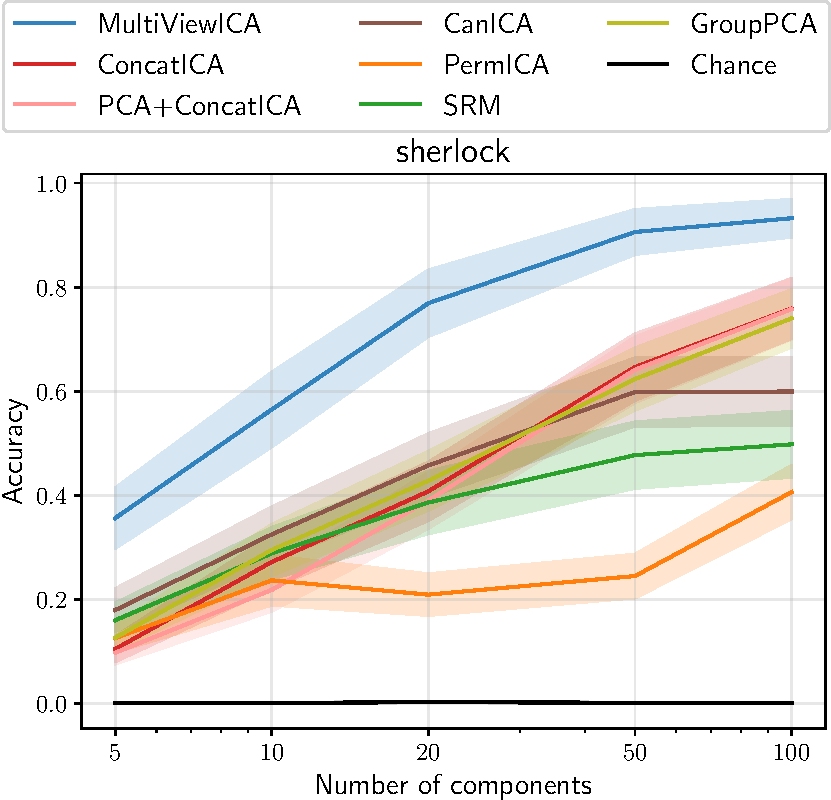
\includegraphics[width=0.6\textwidth]{figures/mvica/timesegment_matching_cae.pdf}
  \caption{\textbf{Reproducing the time-segment matching experiment of \cite{chen2016convolutional}~\cite{zhang2016searchlight}} Mean classification accuracy - error bars represent 95\% confidence interval}
  \label{fig:supp_timesegment}
\end{figure}

\subsection{Impact of the hyperparameter $\sigma$ }
\label{sec:app_sigma_impact}
On top of the theoretical guarantees about the robustness of our method to the choice of the $\sigma$ parameter, we investigate its practical impact on the time-matching segment experiment, on the Sherlock dataset with $10$ components.
%
We compute the accuracy of the multi-view ICA pipeline with different choice of $\sigma$.
%
This is reported in Fig.~\ref{fig:supp_noise_sensitivity}. 
%
The accuracy is constant for a wide range of $\sigma$, only decreasing when $\sigma$ attains very high values.
\begin{figure}
  \centering
  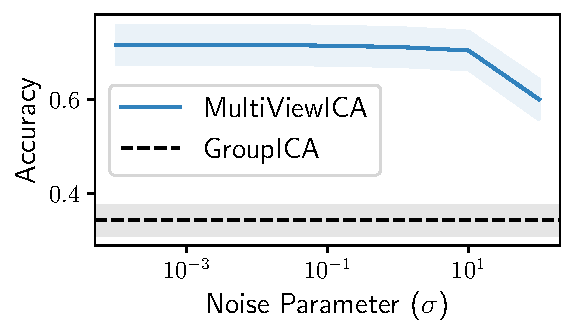
\includegraphics[width=0.6\textwidth]{figures/mvica/noise_sensitivity_reb.pdf}
  \caption{\textbf{Effect of the parameter $\sigma$}: We compute the accuracy of the multiview-ICA pipeline on the time-segment matching experiment for various values of the $\sigma$ hyperparameter over a grid. The accuracy varies only marginally with $\sigma$.}
  \label{fig:supp_noise_sensitivity}
\end{figure}

\section{Related Work}
\label{sec:app_rel_work}
The following table describes some usual method for extracting shared components from multiple subjects datasets.
The column "Modality/Components" describes the type of data for which each algorithm was \emph{initially} proposed, even though each algorithm could be applied on any type of data. 
%
The components type can be either temporal if extracted components are time courses or spatial if they are spatial patterns. 
%
\begin{center}
\begin{longtable}{ |p{.15\textwidth} | p{.2\textwidth} |p{.2\textwidth}| p{.3\textwidth}|}
\hline
\textbf{Method} & \textbf{Modality/Components} &\textbf{Dimension reduction} & \textbf{Description}  \\
\hline
SRM \cite{chen2015reduced} & 
fMRI/Temporal
&
SRM
&
The model is $\xb_i = A_i\sbb + \nb_i$, with \emph{Gaussian} components and \emph{orthogonal} mixing matrices $A_i$\\
\hline
GroupPCA~\cite{smith2014group} &
fMRI/Spatial
&
GroupPCA
&
A memory efficient implementation of PCA applied on temporally concatenated data.\\
\hline
GIFT~ \cite{calhoun2001method} & 
fMRI/Spatial
&
Individual PCA + Group PCA (on component-wise concatenated data)
&
Single-subject ICA is applied on the aggregated data\\
\hline
EEGIFT~ \cite{eichele2011eegift} & 
EEG/Temporal
&
Individual PCA + Group PCA (on component-wise concatenated data)
&
Single-subject ICA is applied on the aggregated data\\
\hline
PermICA &
Any
&
Any
&
Single-subject ICA is applied on each subject's data, and the components are matched using the Hungarian algorithm\\
\hline
Clustering approach~\cite{esposito2005independent}&
fMRI/Spatial
&
Individual PCA
&
Single-subject ICA is applied on each subject's data, and the components are matched using a hierarchical clustering algorithm.\\
\hline
Measure projection analysis~\cite{bigdely2013measure}&
EEG/Temporal
&
Individual PCA
&
Single-subject ICA is applied on each subject's data, and the components are matched using a hierarchical clustering algorithm.\\
\hline
TensorICA \cite{beckmann2005tensorial} &
fMRI/Spatial
&
Group PCA (on spatially concatenated data)
&
TensorICA incorporates ICA assumptions into the PARAFAC model. The mixing matrices $A_1 \cdots A_n$ are such that $A_i = A D_i$ where $A$ is common to all subjects and $D_i$ are subject specific diagonal matrices.\\  
\hline
Unifying Approach of \cite{guo2008unified} &
fMRI/Spatial
&
Group PCA (on spatially concatenated data) + GroupPCA (on component-wise concatenated data).
&
The model is $\xb_i = A_i\sbb + \nb_i$ with a Gaussian mixture model on independent components and a matrix normal prior on the noise. \\
\hline
SR-ICA \cite{zhang2016searchlight} &
fMRI/Temporal
&
SR-ICA
&
SR-ICA incorporates ICA assumptions into the shared response model.  \\
\hline
CAE-SRM \cite{chen2016convolutional}
&
fMRI/Temporal
&
CAE-SRM
&
A convolutional auto-encoder is used to perform the unmixing. \\  
\hline
CanICA \cite{varoquaux2009canica} &
fMRI/Spatial
&
Individual PCA + multi set CCA (on component-wise concatenated data)
&
CanICA applies single-subject ICA on data reduced with PCA and CCA.
 \\  
\hline
Spatial ConcatICA~\cite{svensen2002ica} &
fMRI/Spatial
&
Group PCA (on spatially concatenated data)
&
ICA is applied on spatially concatenated data. The mixing is constrained to be the same across all subjects.
 \\  
 \hline
Temporal ConcatICA~\cite{cong2013validating} &
EEG/Temporal
&
Group PCA (on temporally concatenated data)
&
ICA is applied on temporaly concatenated data. The mixing is constrained to be the same across all subjects.
 \\  
\hline
coroICA \cite{pfister2019robustifying} &
Any
&
Any
&
The model is  $\xb_i = A\sbb_i + \nb_i$. The mixing is constrained to be the same across all subjects. \\
%\hline
%Arbitrary correlation factor analysis of~\cite{Monti18UAI} &
%fMRI/Temporal &
%Any &
%The probabilistic model of~\cite{Monti18UAI} assumes the mixing matrix is orthogonal, positive and shared across subjects but not necessarily square. It learns subjects specific co-variance matrices.  \\
\hline
\end{longtable}
\end{center}
\vspace{-10mm}
An additional related model is described in~\cite{gresele2019incomplete}. Similarly to our work, the ICA model has noise on the components side. However, the model involves nonlinear mixings, which are computationally unfeasible to optimize via maximum likelihood; a contrastive learning scheme is therefore adopted, and the likelihood is not derived in closed form. No evaluation on neuroimaging datasets is presented.

\section{Detailed Cam-CAN components}
\label{sec:app_montages}
We display each of the 11 shared components found by Multiview ICA on the Cam-CAN. The time-courses are on the left, the corresponding brain maps are on the right.


{\centering
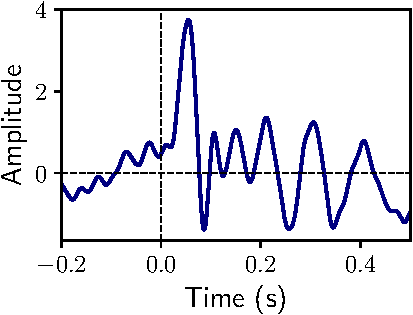
\includegraphics[width=0.3\textwidth]{figures/mvica/camcan_source_0.pdf}%
\raisebox{0.2\height}{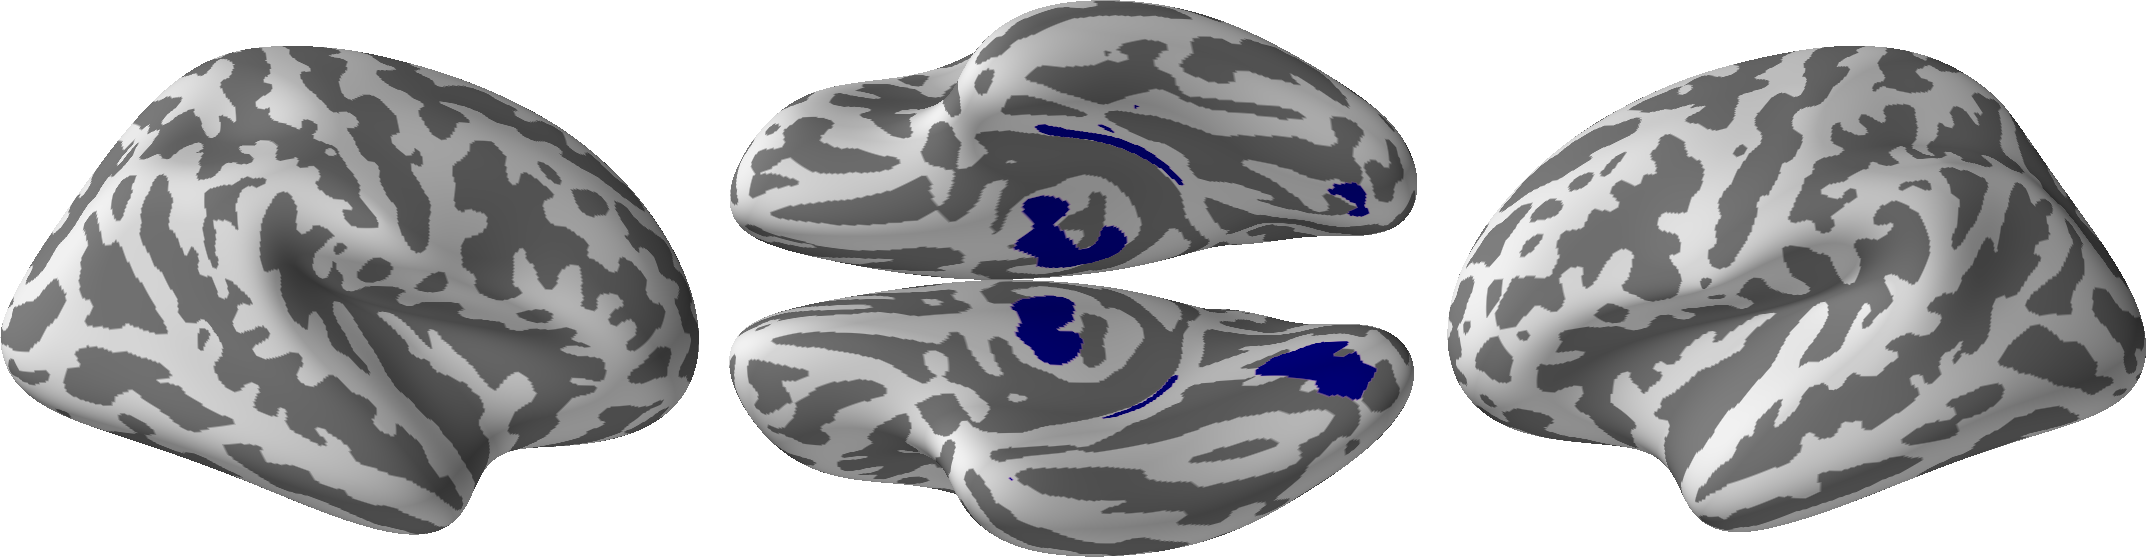
\includegraphics[width=0.68\textwidth]{figures/mvica/montage_0.png}} \\
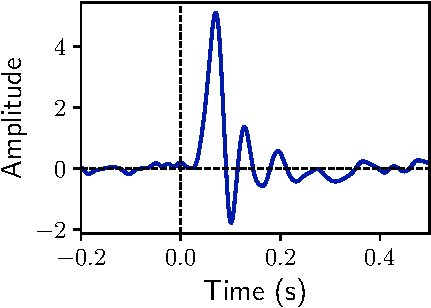
\includegraphics[width=0.3\textwidth]{figures/mvica/camcan_source_1.pdf}%
\raisebox{0.2\height}{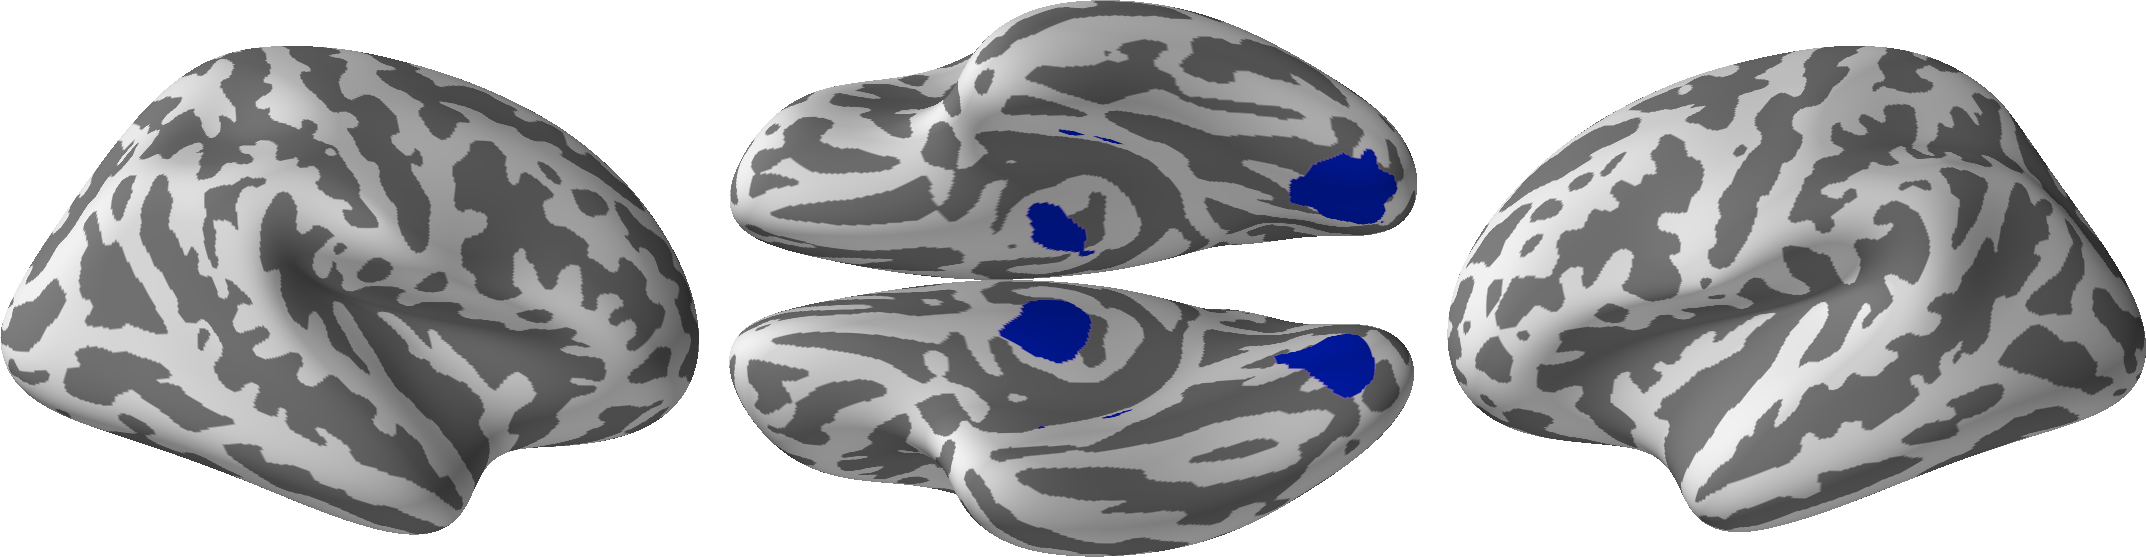
\includegraphics[width=0.68\textwidth]{figures/mvica/montage_1.png}} \\
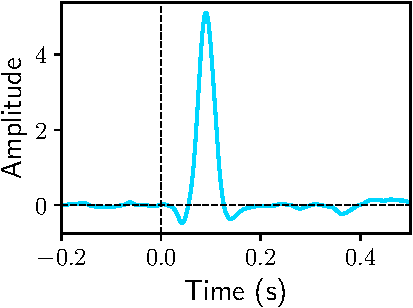
\includegraphics[width=0.3\textwidth]{figures/mvica/camcan_source_2.pdf}%                        
\raisebox{0.2\height}{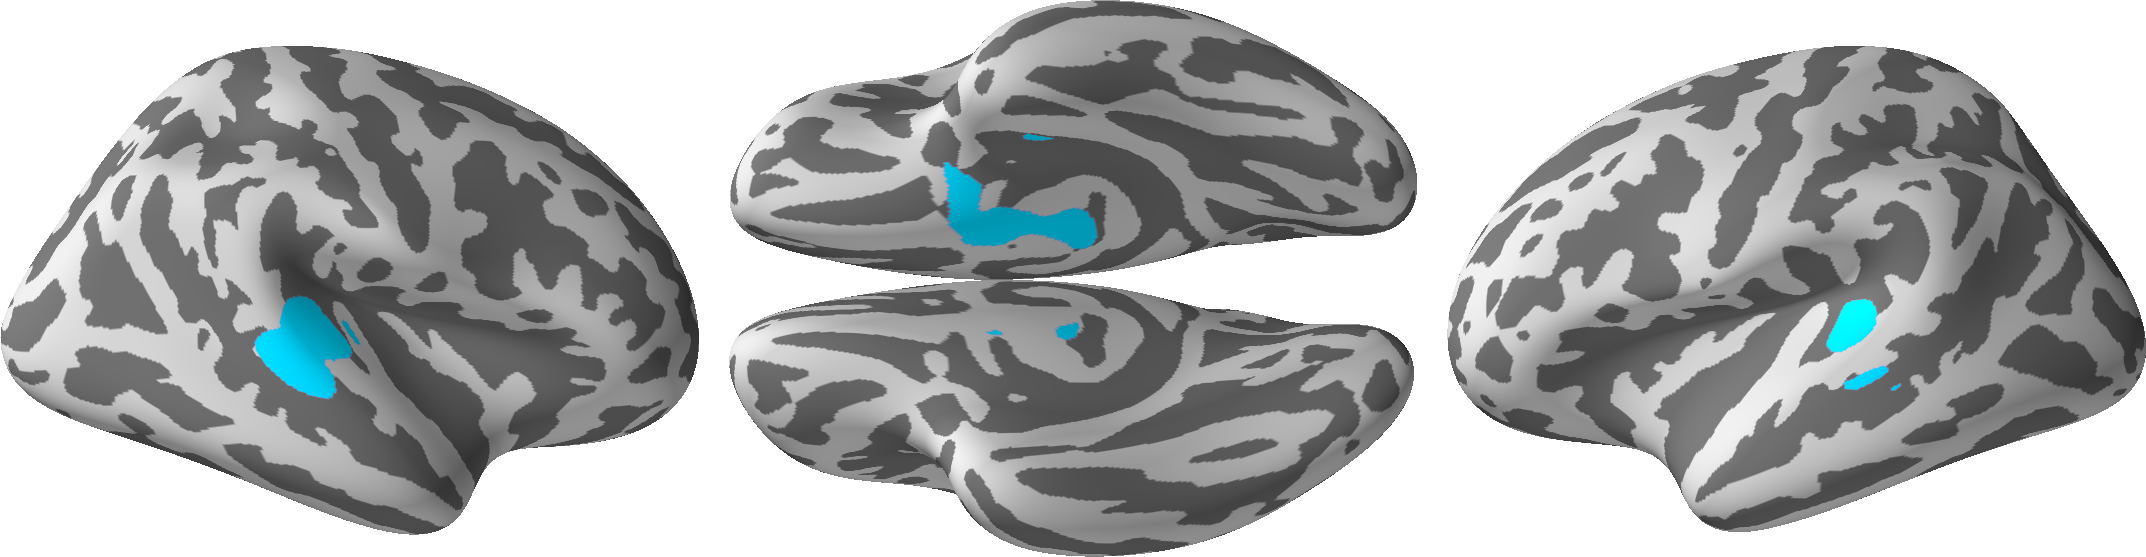
\includegraphics[width=0.68\textwidth]{figures/mvica/montage_2.png}} \\
\includegraphics[width=0.3\textwidth]{figures/mvica/camcan_source_3.pdf}%  
\raisebox{0.2\height}{\includegraphics[width=0.68\textwidth]{figures/mvica/montage_3.png}} \\
\includegraphics[width=0.3\textwidth]{figures/mvica/camcan_source_4.pdf}%
\raisebox{0.2\height}{\includegraphics[width=0.68\textwidth]{figures/mvica/montage_4.png}} \\
\includegraphics[width=0.3\textwidth]{figures/mvica/camcan_source_5.pdf}%
\raisebox{0.2\height}{\includegraphics[width=0.68\textwidth]{figures/mvica/montage_5.png}} \\
\includegraphics[width=0.3\textwidth]{figures/mvica/camcan_source_6.pdf}%
\raisebox{0.2\height}{\includegraphics[width=0.68\textwidth]{figures/mvica/montage_6.png}} \\
\includegraphics[width=0.3\textwidth]{figures/mvica/camcan_source_7.pdf}%
\raisebox{0.2\height}{\includegraphics[width=0.68\textwidth]{figures/mvica/montage_7.png}} \\
\includegraphics[width=0.3\textwidth]{figures/mvica/camcan_source_8.pdf}%
\raisebox{0.2\height}{\includegraphics[width=0.68\textwidth]{figures/mvica/montage_8.png}} \\
\includegraphics[width=0.3\textwidth]{figures/mvica/camcan_source_9.pdf}%
\raisebox{0.2\height}{\includegraphics[width=0.68\textwidth]{figures/mvica/montage_9.png}} \\
\includegraphics[width=0.3\textwidth]{figures/mvica/camcan_source_10.pdf}%
\raisebox{0.2\height}{\includegraphics[width=0.68\textwidth]{figures/mvica/montage_10.png}} \\
}

\section{Average forward operators on fMRI datasets}
\label{sec:spatial_maps}
We display the average forward operator across subjects on the Raiders, Forrest, Clips and Sherlock datasets obtained with MultiViewICA and GroupICA with 5 components. A 5~mm spatial smoothing was applied on all datasets, and the confound signals corresponding to the 5 components with the highest variance were removed before applying MultiViewICA or GroupICA.

{\centering

  \includegraphics[width=\textwidth]{figures/mvica/maps_forrest.png} \\
  \includegraphics[width=\textwidth]{figures/mvica/maps_sherlock.png} \\
  \includegraphics[width=\textwidth]{figures/mvica/maps_gallant.png} \\
  \includegraphics[width=\textwidth]{figures/mvica/maps_raiders.png} \\
}

\section{Synthetic benchmark using the model $\xb_i = A_i\sbb + \nb_i$}
\label{app:complex_cov}
We generate data according to the model $\xb_i = A_i\sbb + \nb_i$, where $\xb_i \in \mathbb{R}^{50}$, $\sbb \in \mathbb{R}^{20}$, and $\nb_i\sim \mathcal{N}(0, \sigma^2 I_{50})$. After applying individual PCA to obtain signals of dimension $20$, we apply the different ICA algorithms and report the reconstruction error in fig.~\ref{fig:reconstruction_synth}.

\begin{figure}
  \center
  \includegraphics[width=0.5\linewidth]{figures/mvica/distance.pdf}
  \caption{Synthetic experiment with model $\xb_i = A_i\sbb^i + \nb_i$} %{Light Unit}
  \label{fig:reconstruction_synth}
\end{figure}

\section{Summary of our quantitative results}
\label{sec:app_real_data}
Our quantitative results for the fMRI experiments of time-segment matching and BOLD signal reconstruction and on for the MEG phantom data experiment are summarized, respectively, in Table~\ref{tab:timeseg}, Table~\ref{tab:recon} and Table~\ref{tab:meg}. All methods are compared upon extraction of components with the same dimensionality ($20$ components).

\begin{table}
    \centering
    \begin{tabular}{|c|c | c | c|}
            \hline
         \textbf{Dataset} & \textbf{Method} & \textbf{Accuracy} & \textbf{Confidence interval} \\
         \hline
clips   & Chance      & 0.002&[0.001, 0.003] \\
        & CanICA    & 0.130&[0.112, 0.147] \\
        & PCA + GroupICA      & 0.124&[0.109, 0.139] \\
        & GroupICA    & 0.152&[0.133, 0.171] \\

        & PermICA     & 0.147&[0.126, 0.169] \\
        & SRM         & 0.115&[0.104, 0.126] \\
        & MultiViewICA& \textbf{0.167}&[0.142, 0.192] \\
        \hline
forrest & Chance      & 0.002&[0.001, 0.002] \\
        & CanICA    & 0.192&[0.170, 0.214] \\
        & PCA + GroupICA      & 0.088&[0.077, 0.098] \\
        & GroupICA    & 0.154&[0.137, 0.170] \\
        & PermICA     & 0.135&[0.118, 0.152] \\
        & SRM         & 0.188&[0.173, 0.203] \\
        & MultiViewICA& \textbf{0.448}&[0.411, 0.484] \\
        \hline
raiders & Chance      & 0.002&[0.001, 0.003] \\
        & CanICA    & 0.256&[0.220, 0.291] \\
        & PCA + GroupICA      & 0.331&[0.289, 0.372] \\
        & GroupICA    & 0.321&[0.281, 0.361] \\
        & PermICA     & 0.381&[0.341, 0.421] \\
        & SRM         & 0.265&[0.240, 0.289] \\
         & MultiViewICA& \textbf{0.408}&[0.358, 0.458] \\
         \hline
sherlock& Chance      & 0.005&[0.003, 0.006] \\
        & CanICA    & 0.607&[0.567, 0.648] \\
        & PCA + GroupICA      & 0.454&[0.416, 0.492] \\
        & GroupICA    & 0.519&[0.481, 0.556] \\
        & PermICA     & 0.399&[0.365, 0.434] \\
        & SRM         & 0.493&[0.465, 0.520] \\
        & MultiViewICA& \textbf{0.873}&[0.844, 0.903] \\
\hline
    \end{tabular}
    \caption{Timesegment matching: Summary of our quantitative results. We report the mean accuracy across cross-validation splits.}
    \label{tab:timeseg}
\end{table}

\begin{table}
    \centering
    \begin{tabular}{|c|c | c | c|}
            \hline
         \textbf{Dataset} & \textbf{Method} & \textbf{R2 score} & \textbf{Confidence interval} \\
         \hline
         clips   & Chance              & 0.000&[0.000 ,0.000] \\
        & CanICA            &  0.110&[ 0.097 , 0.123] \\
        & PCA + GroupICA              &  0.075&[ 0.058 , 0.092] \\
        & GroupICA            &  0.077&[ 0.059 , 0.094] \\
        & PermICA             &  0.099&[ 0.087 , 0.111] \\
        & SRM                 &  0.081&[ 0.069 , 0.094] \\
        & MultiViewICA        &  \textbf{0.114}&[ 0.099 , 0.128] \\
        \hline
forrest & Chance              & 0.000&[0.000 ,0.000] \\
        & CanICA            &  0.181&[ 0.169 , 0.193] \\
        & PCA + GroupICA              &  0.072&[ 0.054 , 0.090] \\
        & GroupICA            &  0.081&[ 0.062 , 0.099] \\
        & PermICA             &  0.098&[ 0.090 , 0.106] \\
        & SRM                 &  0.180&[ 0.168 , 0.193] \\
        & MultiViewICA        &  \textbf{0.191}&[ 0.177 , 0.204] \\
        \hline
raiders & Chance              & 0.000&[0.000 ,0.000] \\
        & CanICA            &  0.136&[ 0.122 , 0.149] \\
        & PCA + GroupICA              &  0.063&[ 0.045 , 0.080] \\
        & GroupICA            &  0.062&[ 0.043 , 0.081] \\
        & PermICA             &  0.107&[ 0.091 , 0.124] \\
        & SRM                 &  0.138&[ 0.121 , 0.154] \\
        & MultiViewICA        &  \textbf{0.144}&[ 0.124 , 0.164] \\
        \hline
sherlock& Chance              & 0.000&[0.000 ,0.000] \\
        & CanICA            &  0.156&[ 0.141 , 0.172] \\
        & PCA + GroupICA              &  0.087&[ 0.065 , 0.108] \\
        & GroupICA            &  0.091&[ 0.070 , 0.112] \\
        & PermICA             &  0.067&[ 0.055 , 0.078] \\
        & SRM                 &  \textbf{0.164}&[ 0.147 , 0.181] \\
        & MultiViewICA        &  0.161&[ 0.142 , 0.180] \\
        \hline

         
    \end{tabular}
    \caption{Reconstructing the BOLD signal of missing subjects: Summary of our quantitative results. We report the mean R2 score across cross-validation splits.}
    \label{tab:recon}
\end{table}

\begin{table}
    \centering
    \begin{tabular}{|c|c|c|c}
    \hline
         \textbf{Method} & \textbf{Reconstruction error} & \textbf{1st and 3d quartiles} 
         \\
         \hline
         MultiViewICA & \textbf{0.0045} & [0.0039, 0.0052] \\ 
GroupICA & 0.1098 & [0.0549, 0.1734] \\ 
PCA+GroupICA & 0.1111 & [0.0760, 0.1502] \\ 
PermICA & 0.0730 & [0.0423, 0.1037] \\ 
\hline
    \end{tabular}
    \caption{Phantom MEG data: Summary of our quantitative results with 2 epochs. We report the median reconstruction error across cross-validation splits.}
    \label{tab:meg}
\end{table}
\chapter{Open source contributions}
\section{Mvlearn}
\section{Brainiak}

\chapter{Analyzing fMRI data of multiple subjects}
\section{The controlled setting: the general linear model}
\section{A deep approach for modeling complex stimuli}
\end{document}